\documentclass{beamer}
\usepackage{amsmath}

\usetheme{Warsaw}


\iftrue

\setbeamercolor{normal text}{fg=white,bg=black!90}
\setbeamercolor{structure}{fg=white}

\setbeamercolor{alerted text}{fg=red!85!black}

\setbeamercolor{item projected}{use=item,fg=black,bg=item.fg!35}

\setbeamercolor*{palette primary}{use=structure,fg=structure.fg}
\setbeamercolor*{palette secondary}{use=structure,fg=structure.fg!95!black}
\setbeamercolor*{palette tertiary}{use=structure,fg=structure.fg!90!black}
\setbeamercolor*{palette quaternary}{use=structure,fg=structure.fg!95!black,bg=black!80}

\setbeamercolor*{framesubtitle}{fg=white}

\setbeamercolor*{block title}{parent=structure,bg=black!60}
\setbeamercolor*{block body}{fg=black,bg=black!10}
\setbeamercolor*{block title alerted}{parent=alerted text,bg=black!15}
\setbeamercolor*{block title example}{parent=example text,bg=black!15}

\fi


\begin{document}

{
    \usebackgroundtemplate
    {
        \vbox to \paperheight{\vfil\hbox to \paperwidth{\hfil

        {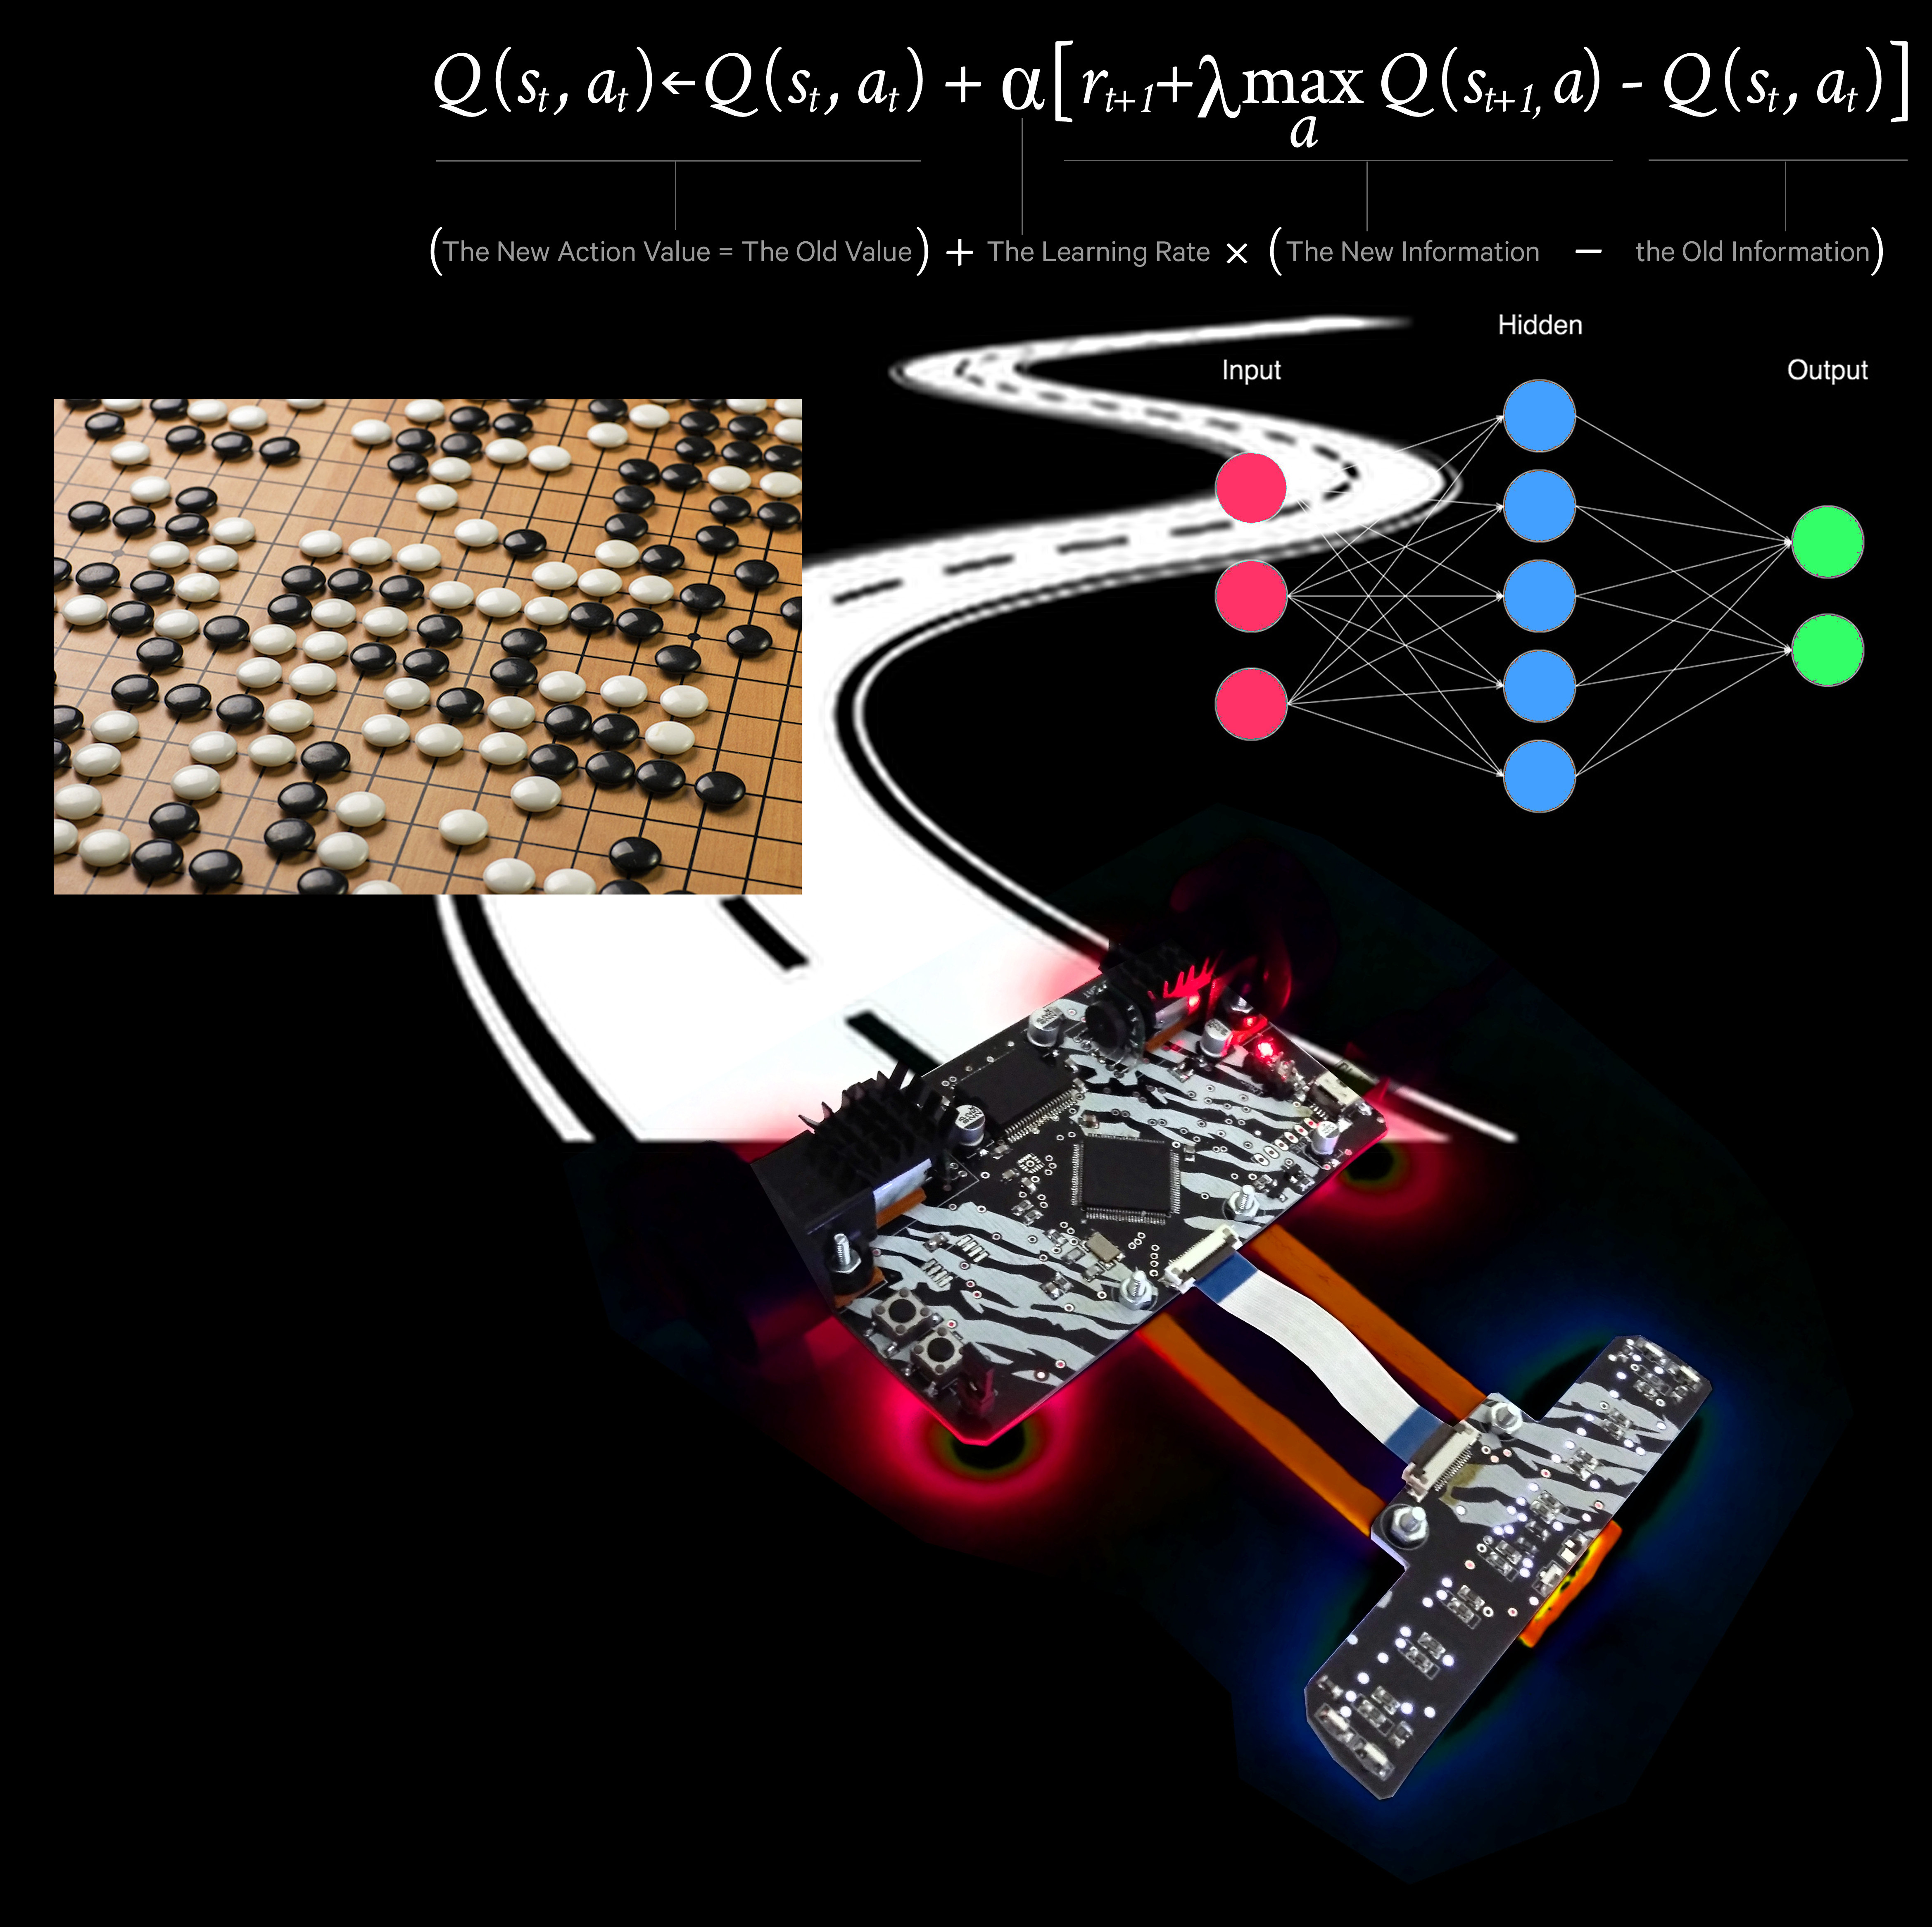
\includegraphics[width=5.05in]{../images/rl_square.jpg}}

        \hfil}\vfil}
    }

    \begin{frame}
     \centering
     \colorbox{black}
     {
        \begin{minipage}{8cm}
           {\LARGE \color{white}{\bf - math }} \\
           {\LARGE \color{white}{\bf - hardware }} \\
           {\LARGE \color{white}{\bf - algorithms  }} \\
           {\LARGE \color{white}{\bf for line following robot}} \\
           {\LARGE \color{white}{\bf Michal CHOVANEC, PhD.}} \\
       \end{minipage}
     }

    \end{frame}
}




\begin{frame}
  
  \frametitle{\bf line following robot}
  
  \begin{columns}

    \begin{column}{0.5\textwidth}
      \centering{\includegraphics[scale=0.045]{../images/istrobot_2024.jpg}}
      \centering{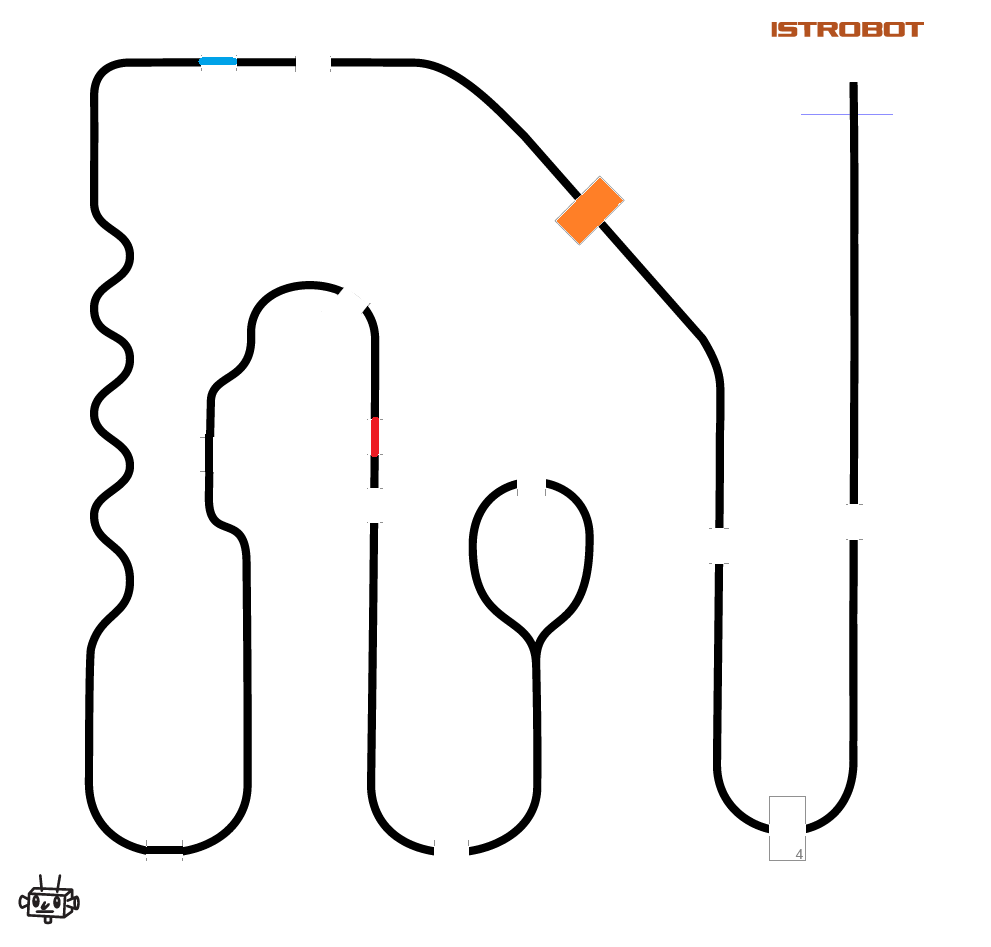
\includegraphics[scale=0.2]{../images/LinefollowerTrack2024.png}}
    \end{column}

    \begin{column}{0.5\textwidth}
      \begin{itemize}
        \item fastest line following
        \item 3 rounds
        \item obstacles : broken line, brick, loop, colored line
      \end{itemize}
    \end{column}

  \end{columns}
  
\end{frame}


\begin{frame}
  
  \frametitle{\bf Istrobot 2024}
  
  \begin{columns}

    \begin{column}{0.5\textwidth}
      \centering{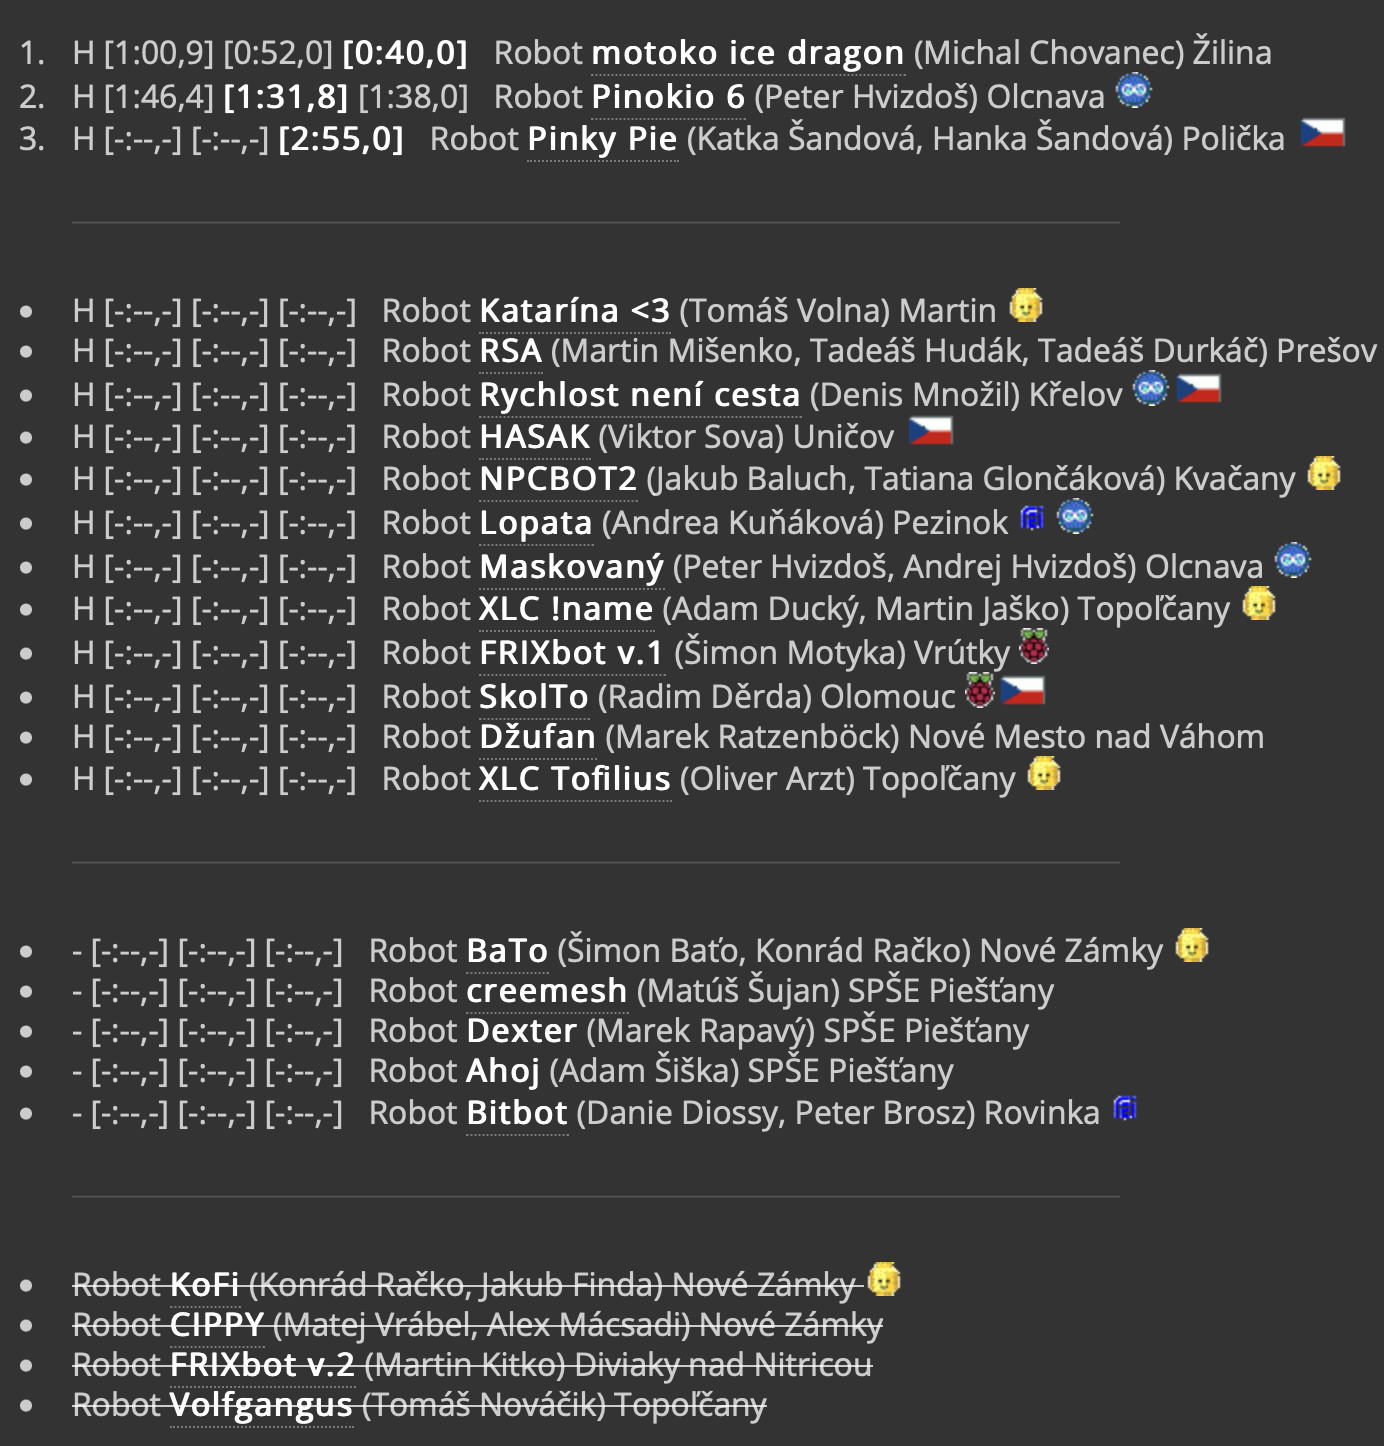
\includegraphics[scale=0.25]{../images/istrobot_2024_results.png}}
    \end{column}

    \begin{column}{0.5\textwidth}
      \begin{itemize}
        \item this category registered total 25 robots
        \item really did particicpate 21, and 15 of them succesfully homologized
        \item out of them, only 3 did succeed at least in one run
        \item just 2 robots did succesfully all three runs
      \end{itemize}
    \end{column}

  \end{columns}
  
\end{frame}




\begin{frame}
  
  \frametitle{\bf DC motor - Pololu.com}

  \begin{columns}

    \begin{column}{0.5\textwidth}
      \centering{\includegraphics[scale=0.04]{../images/motors/dc.jpg}}
    \end{column}

    \begin{column}{0.5\textwidth}
      \begin{itemize}
        \item gear ratio 1:30 (1000 RPM, 0.57kg.cm), item id 2212
        \item gear ratio 1:50 (590 RPM,  0.86kg.cm), item id 2213
        \item 1.6A stall current
        \item magnetic encoder
        \item {\color{red} \bf{ NEVER }} buy cheep alternative 
          - looks same, but gears have pure quality, and torque is less than 50\% !!! 
      \end{itemize}
    \end{column}

  \end{columns}
  
\end{frame}




\begin{frame}
  
  \frametitle{\bf brushless motor - 3phase motor}

  \begin{columns}

    \begin{column}{0.5\textwidth}
      \centering{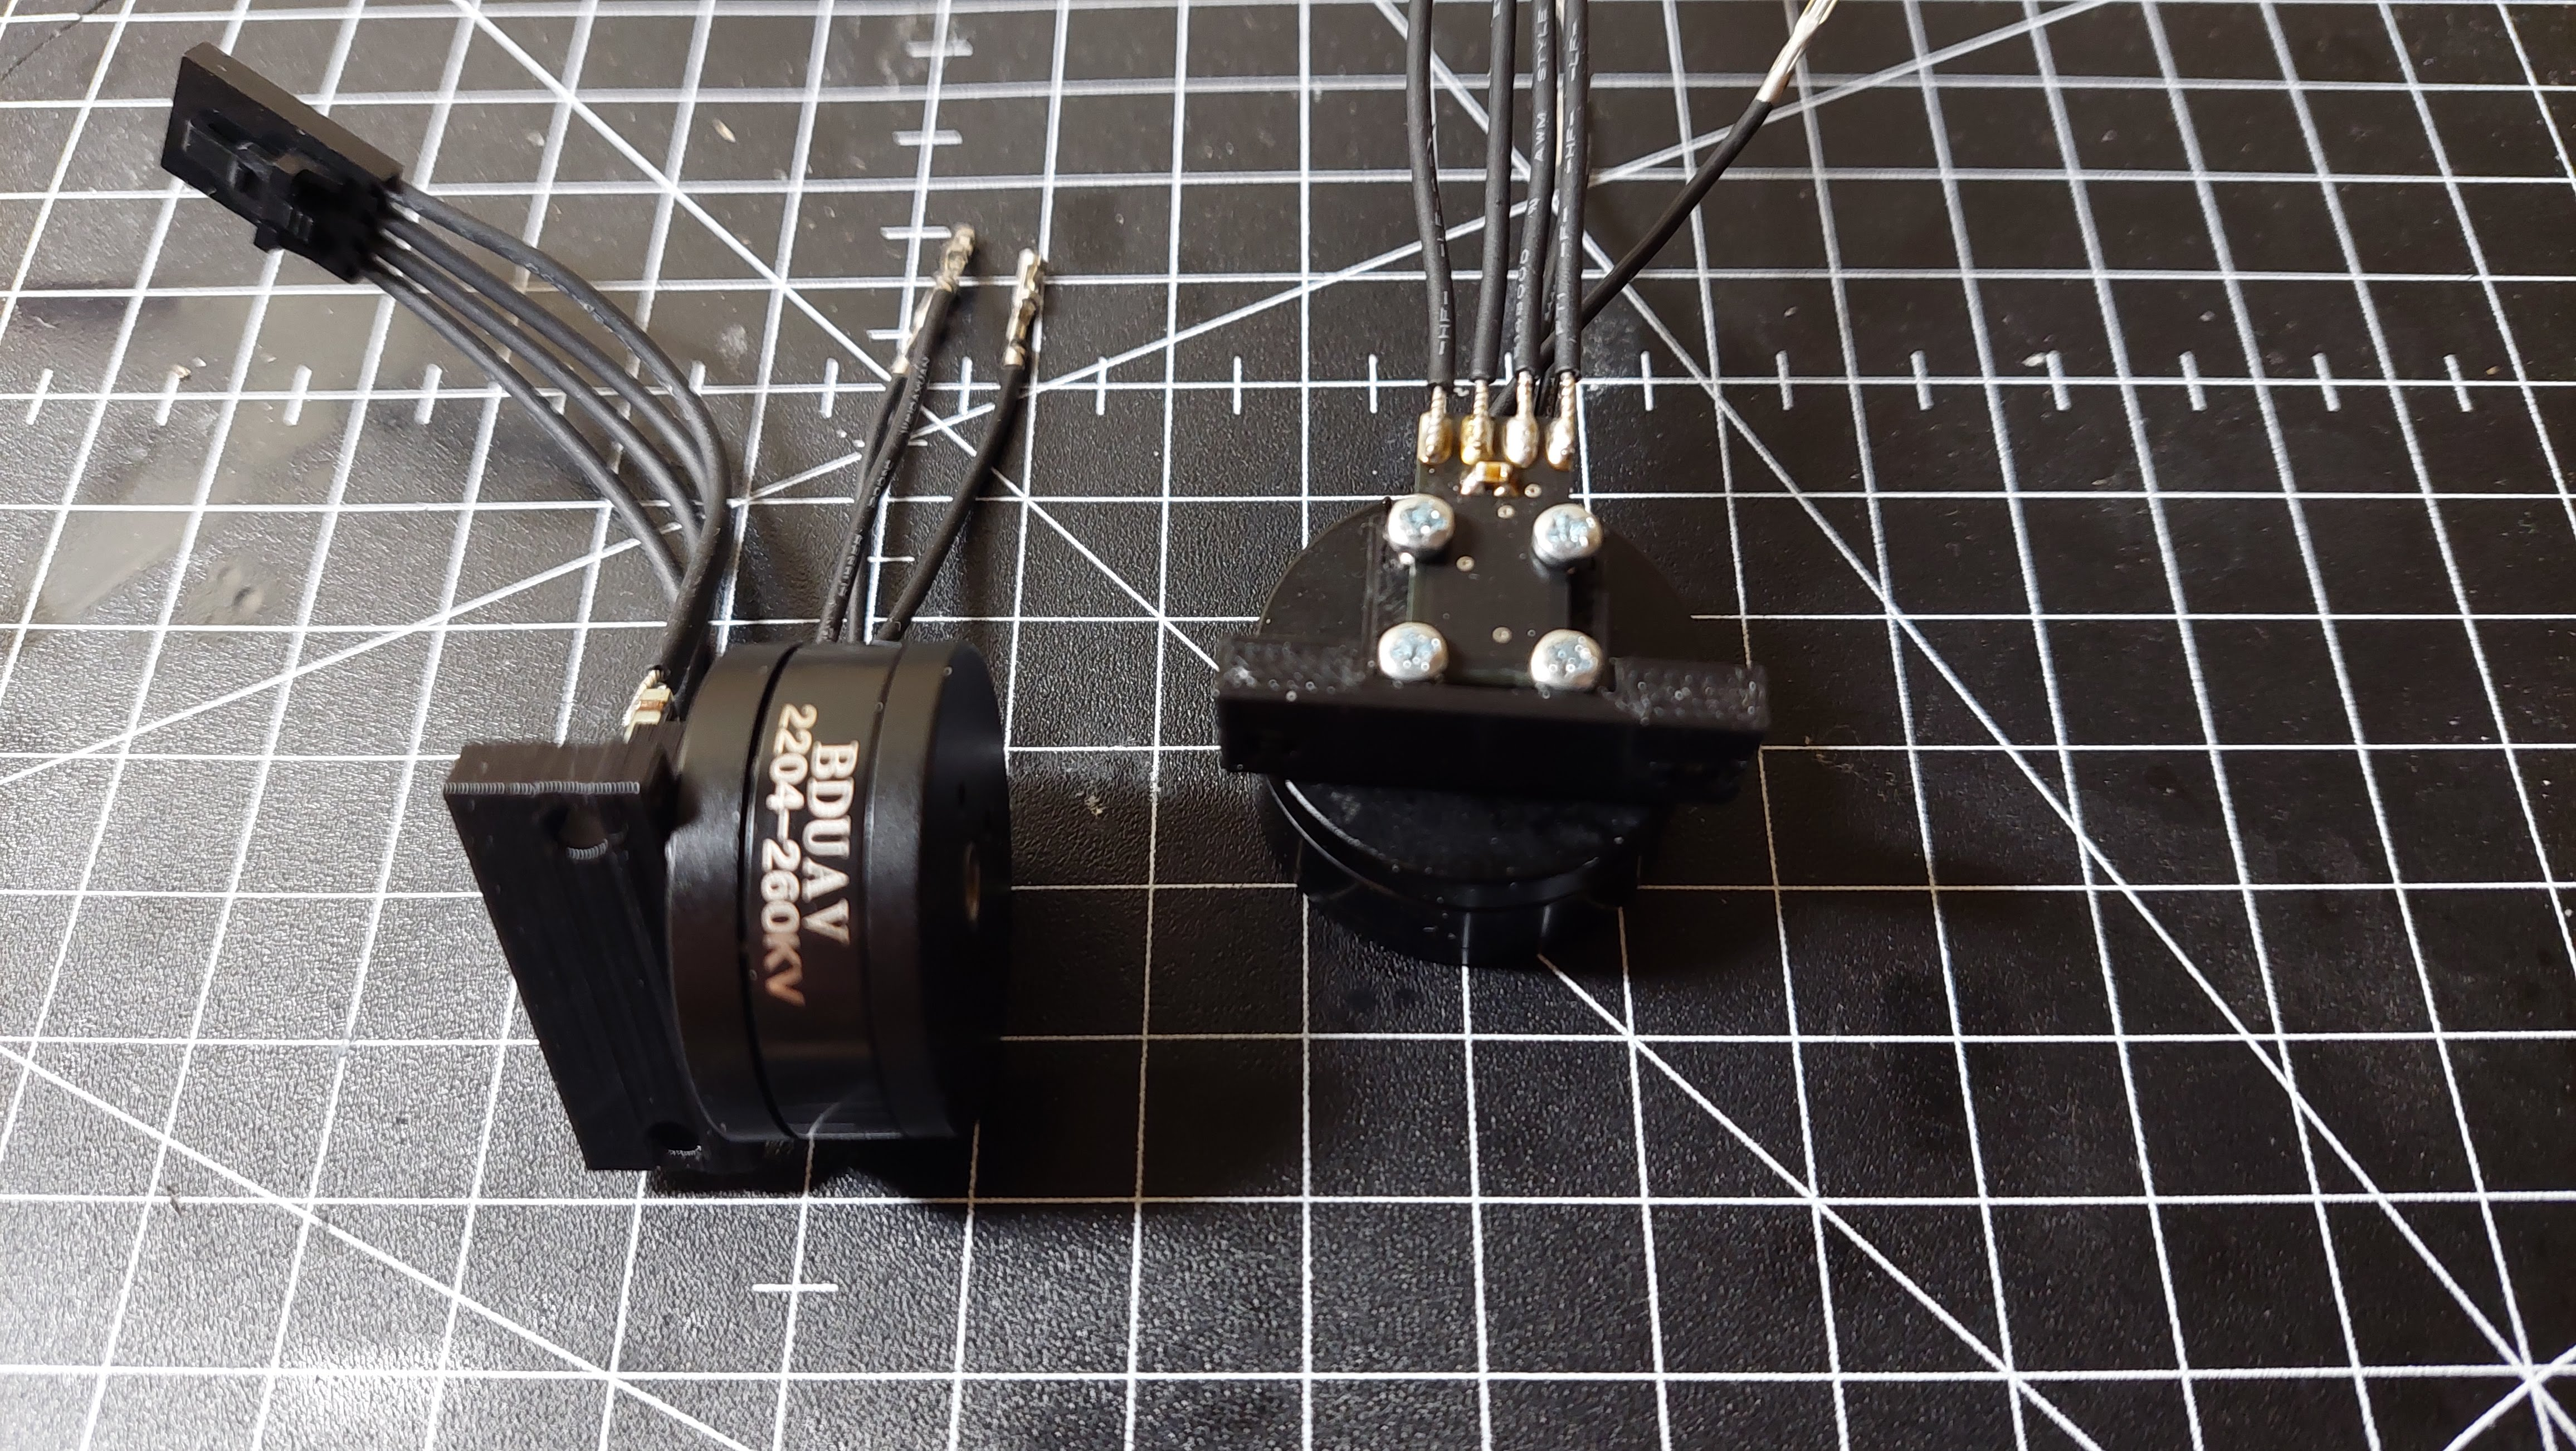
\includegraphics[scale=0.04]{../images/motors/brushless_1.jpg}}
    \end{column}

    \begin{column}{0.5\textwidth}
      \begin{itemize}
        \item use "slow" gimbal motors or outrunner for drone
        \item custom encoder
        \item custom tire
        \item extreme huge power - limited by temperature, and core magnetic saturation
        \item fast response ($\tau = 10ms$)
       
      \end{itemize}
    \end{column}

  \end{columns}
  
\end{frame}




\begin{frame}
  
  \frametitle{\bf brushless motor - 3phase motor}

  \centering{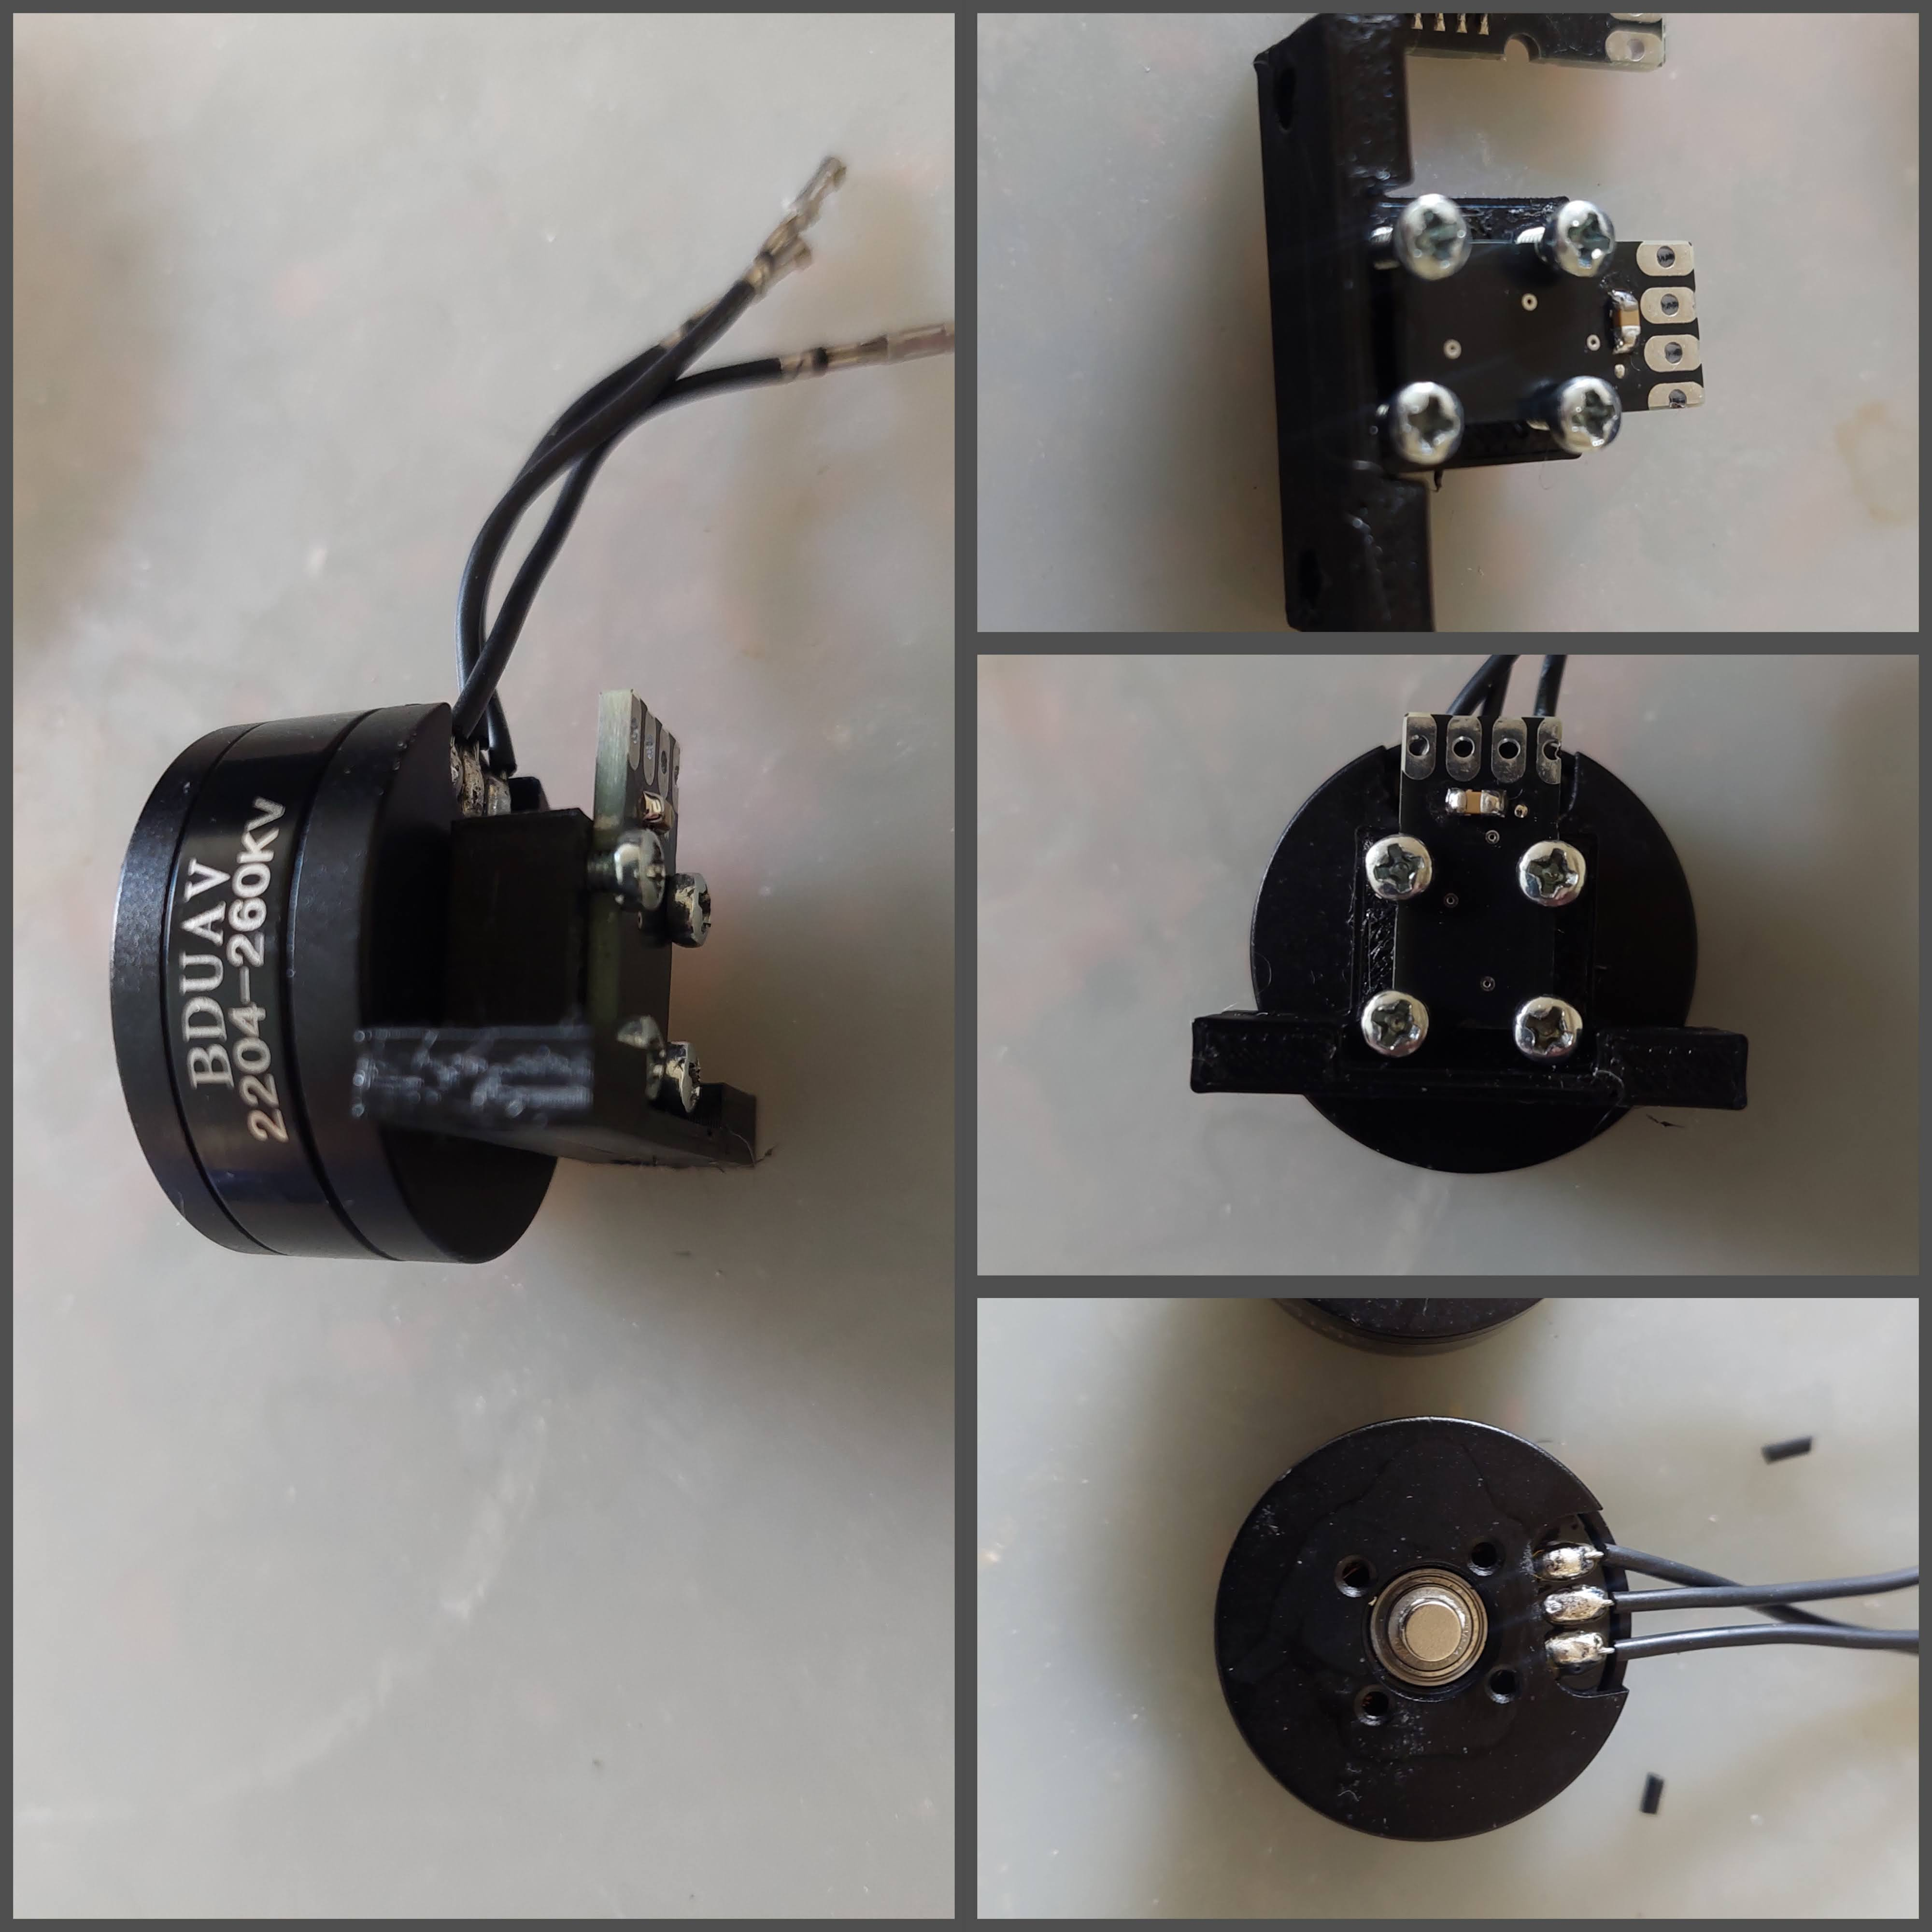
\includegraphics[scale=0.06]{../images/motors/brushless_2.jpg}}
  
\end{frame}




\begin{frame}
  
  \frametitle{\bf motor driver}


  \begin{columns}

    \begin{column}{0.5\textwidth}
      \centering{\includegraphics[scale=0.07]{../images/motors/drivers.jpg}}
    \end{column}

    \begin{column}{0.5\textwidth}
      \begin{itemize}
        \item DC motor
          \begin{itemize}
            \item DRV8213
            \item 4A, 1.65V .. 11V
            \item 40W
          \end{itemize}
        \item Brushless motor
          \begin{itemize}
            \item MP6541
            \item 8A, 4.75V .. 40V
            \item 96W
          \end{itemize}
        \item L293, L298
          - obsolete 19th century devices
      \end{itemize}
    \end{column}

  \end{columns}

\end{frame}



\begin{frame}
  
  \frametitle{\bf FOC - field oriented control}
  

  \begin{columns}

    \begin{column}{0.5\textwidth}
      \centering{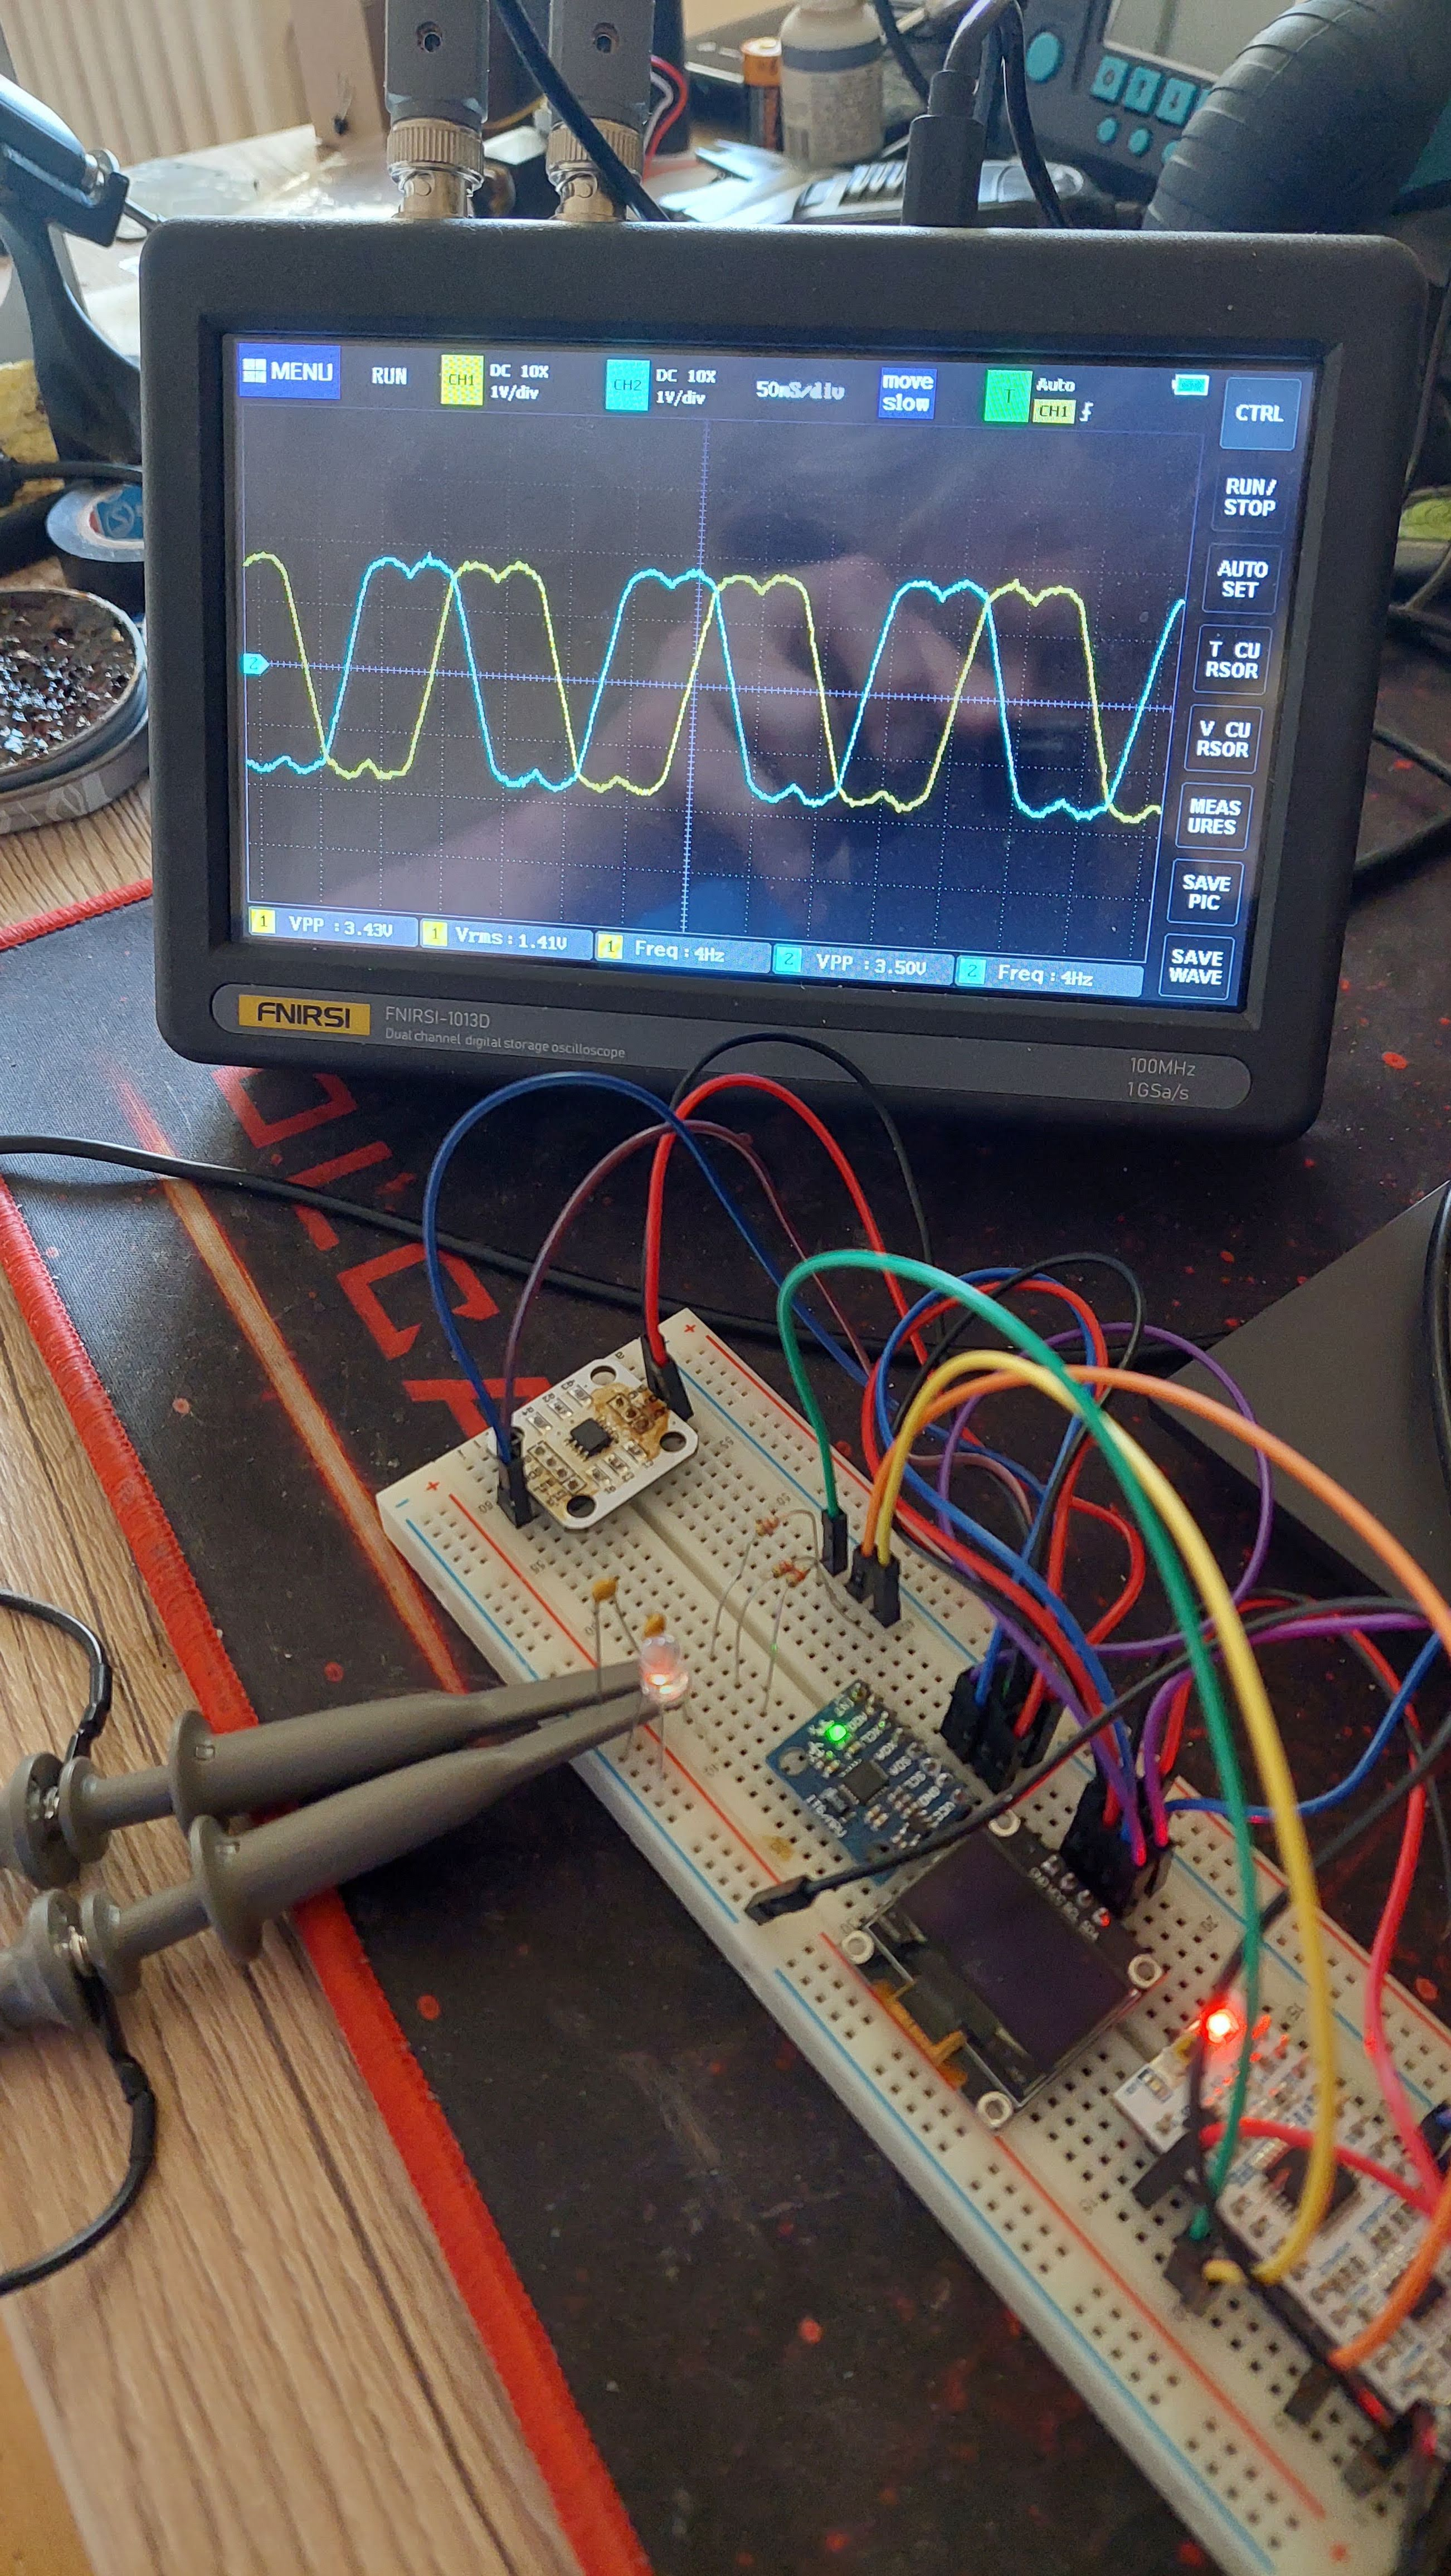
\includegraphics[scale=0.05]{../images/motors/currents.jpg}}
    \end{column}

    \begin{column}{0.5\textwidth}
      \centering{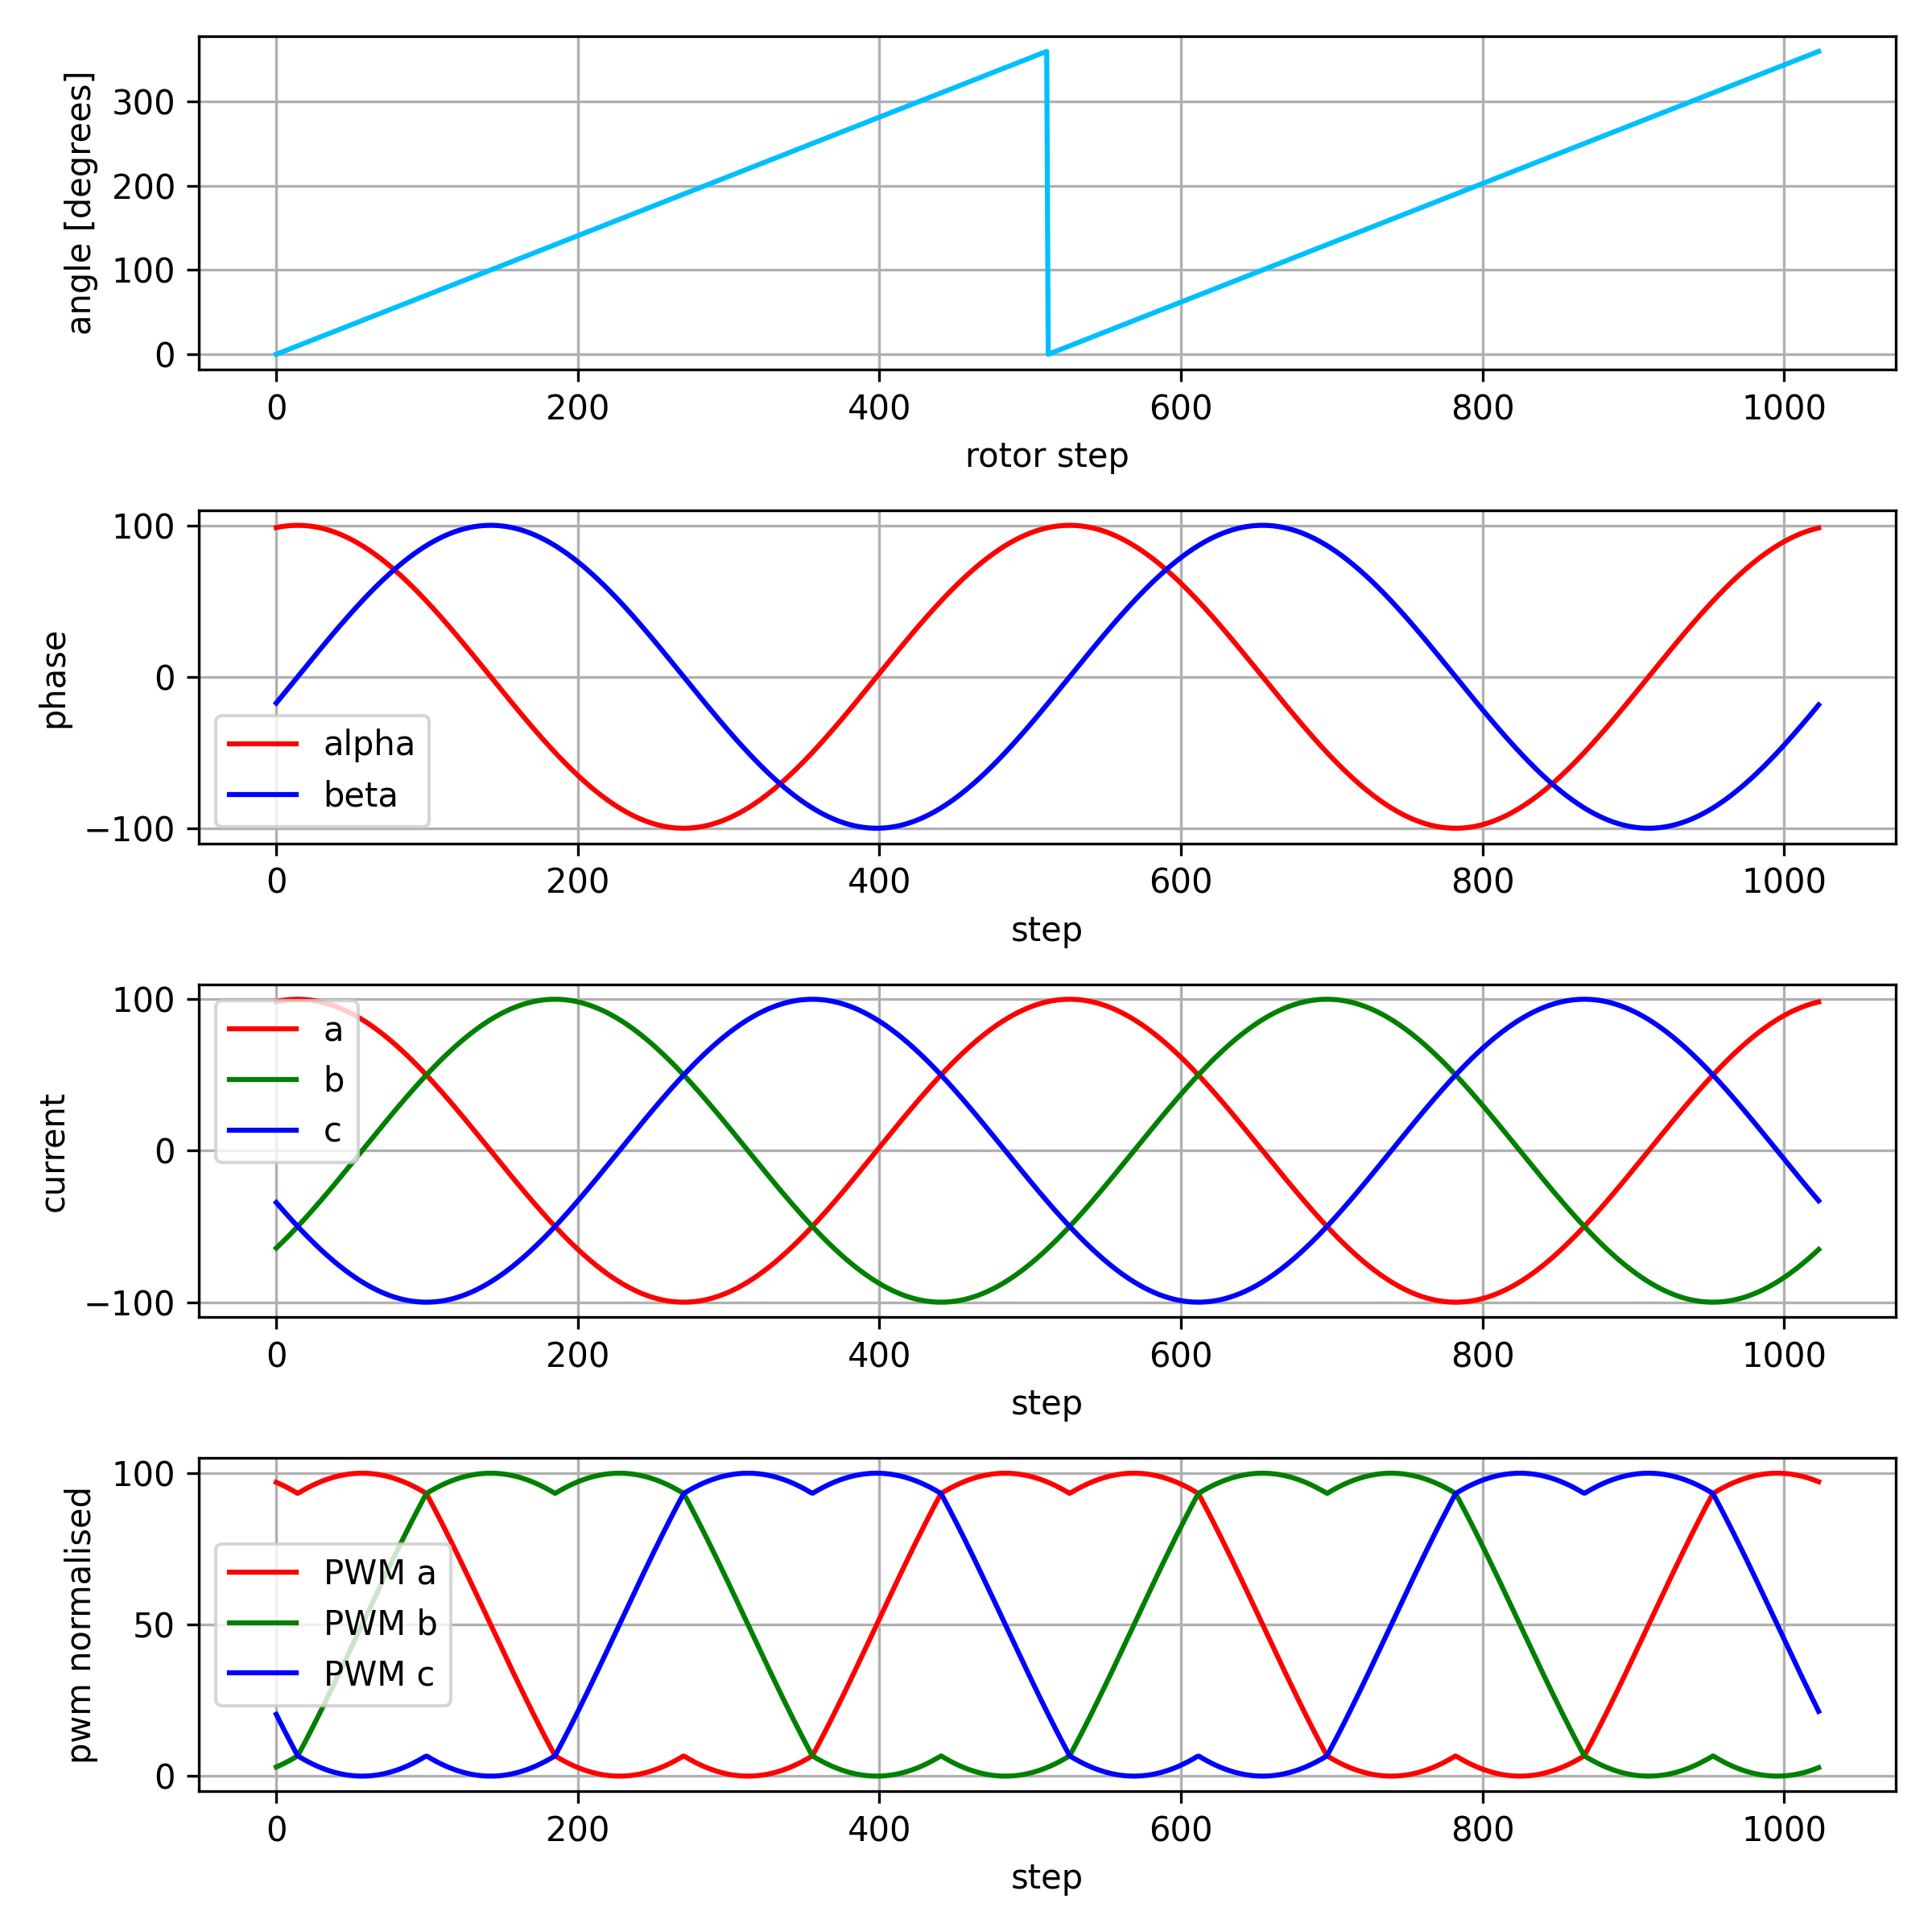
\includegraphics[scale=0.25]{../images/motors/transformations.png}}
    \end{column}

  \end{columns}

\end{frame}


\begin{frame}
  
  \frametitle{\bf FOC - field oriented control}

  \centering{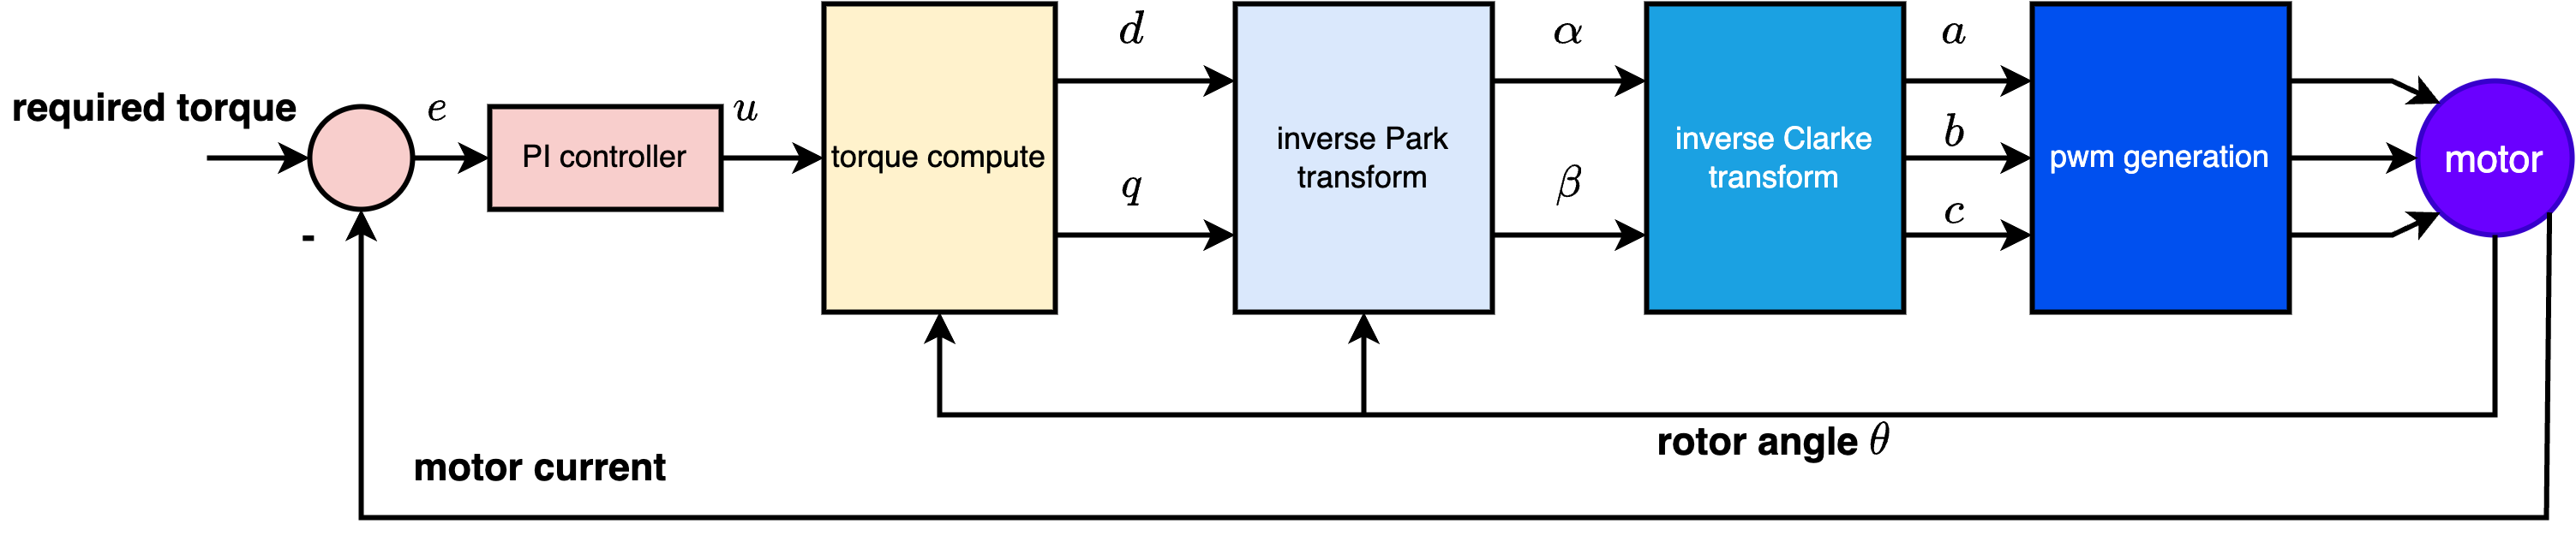
\includegraphics[scale=0.4]{../images/motors/motor_control-inner_loop.png}}
  follow my tutorial \url{https://github.com/michalnand/brushless_motor_control}
\end{frame}


\begin{frame}
  
  \frametitle{\bf FOC - field oriented control}

  \centering{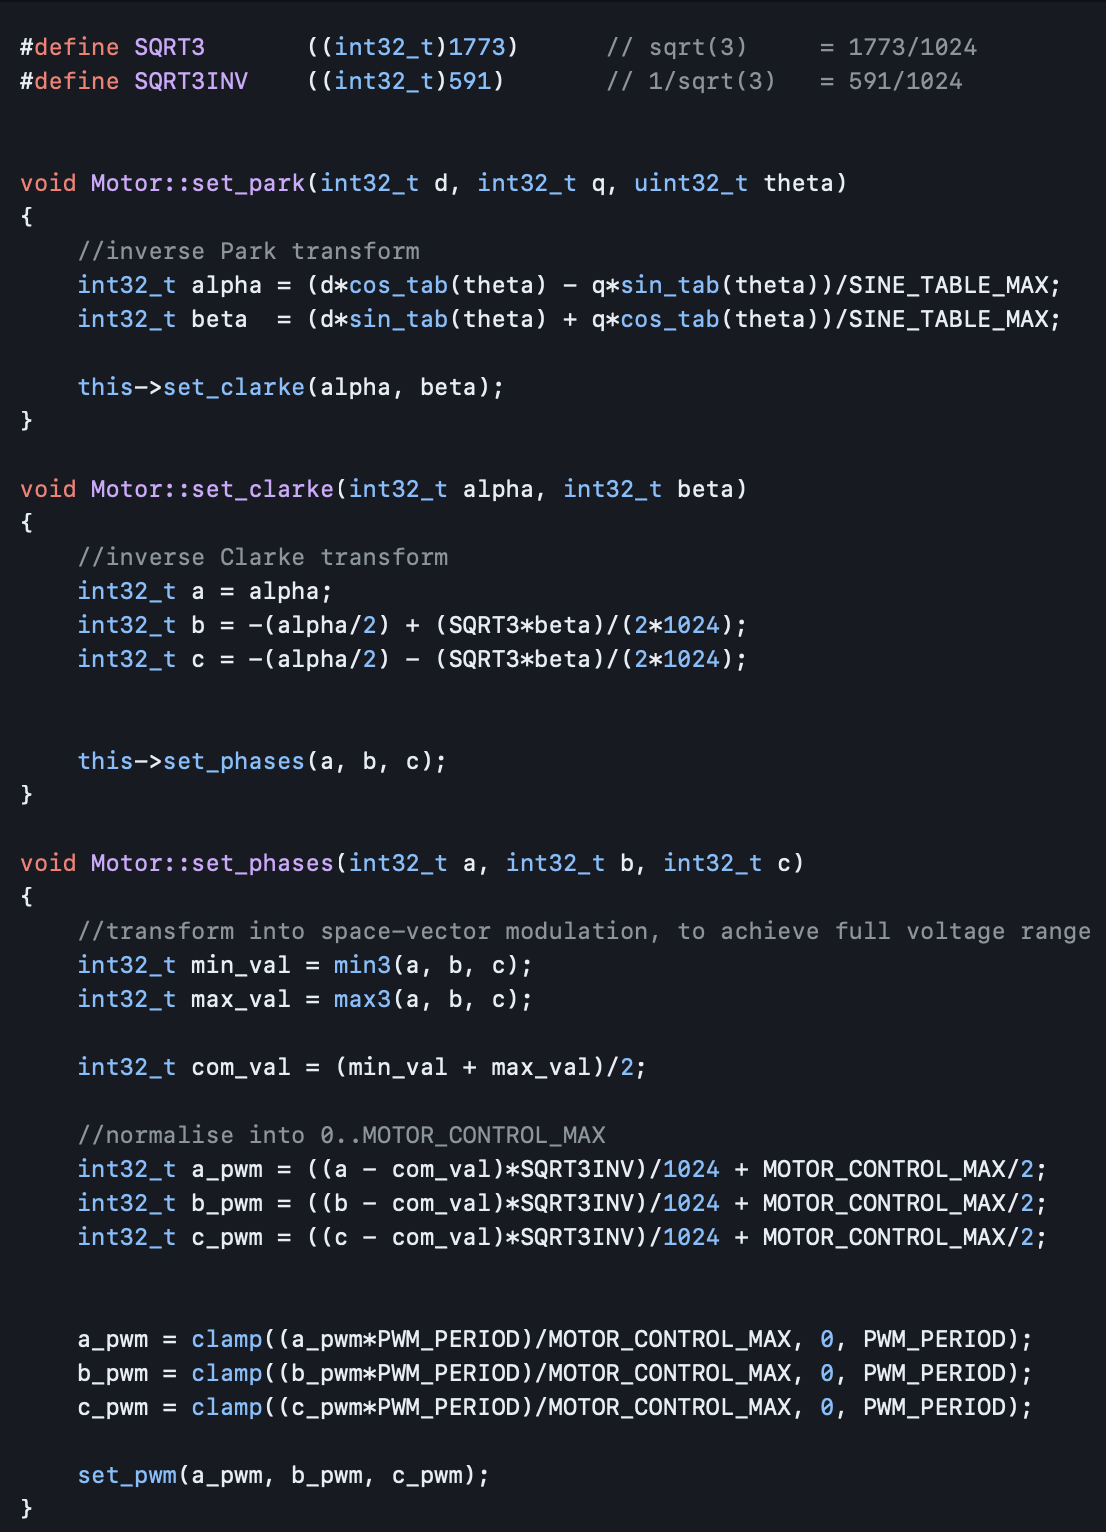
\includegraphics[scale=0.3]{../images/motors/fixed_point_foc.png}}
\end{frame}


\begin{frame}
  
  \frametitle{\bf making custom silicone tires}
  \url{https://www.kaufland.sk/product/482387287/}

  \centering{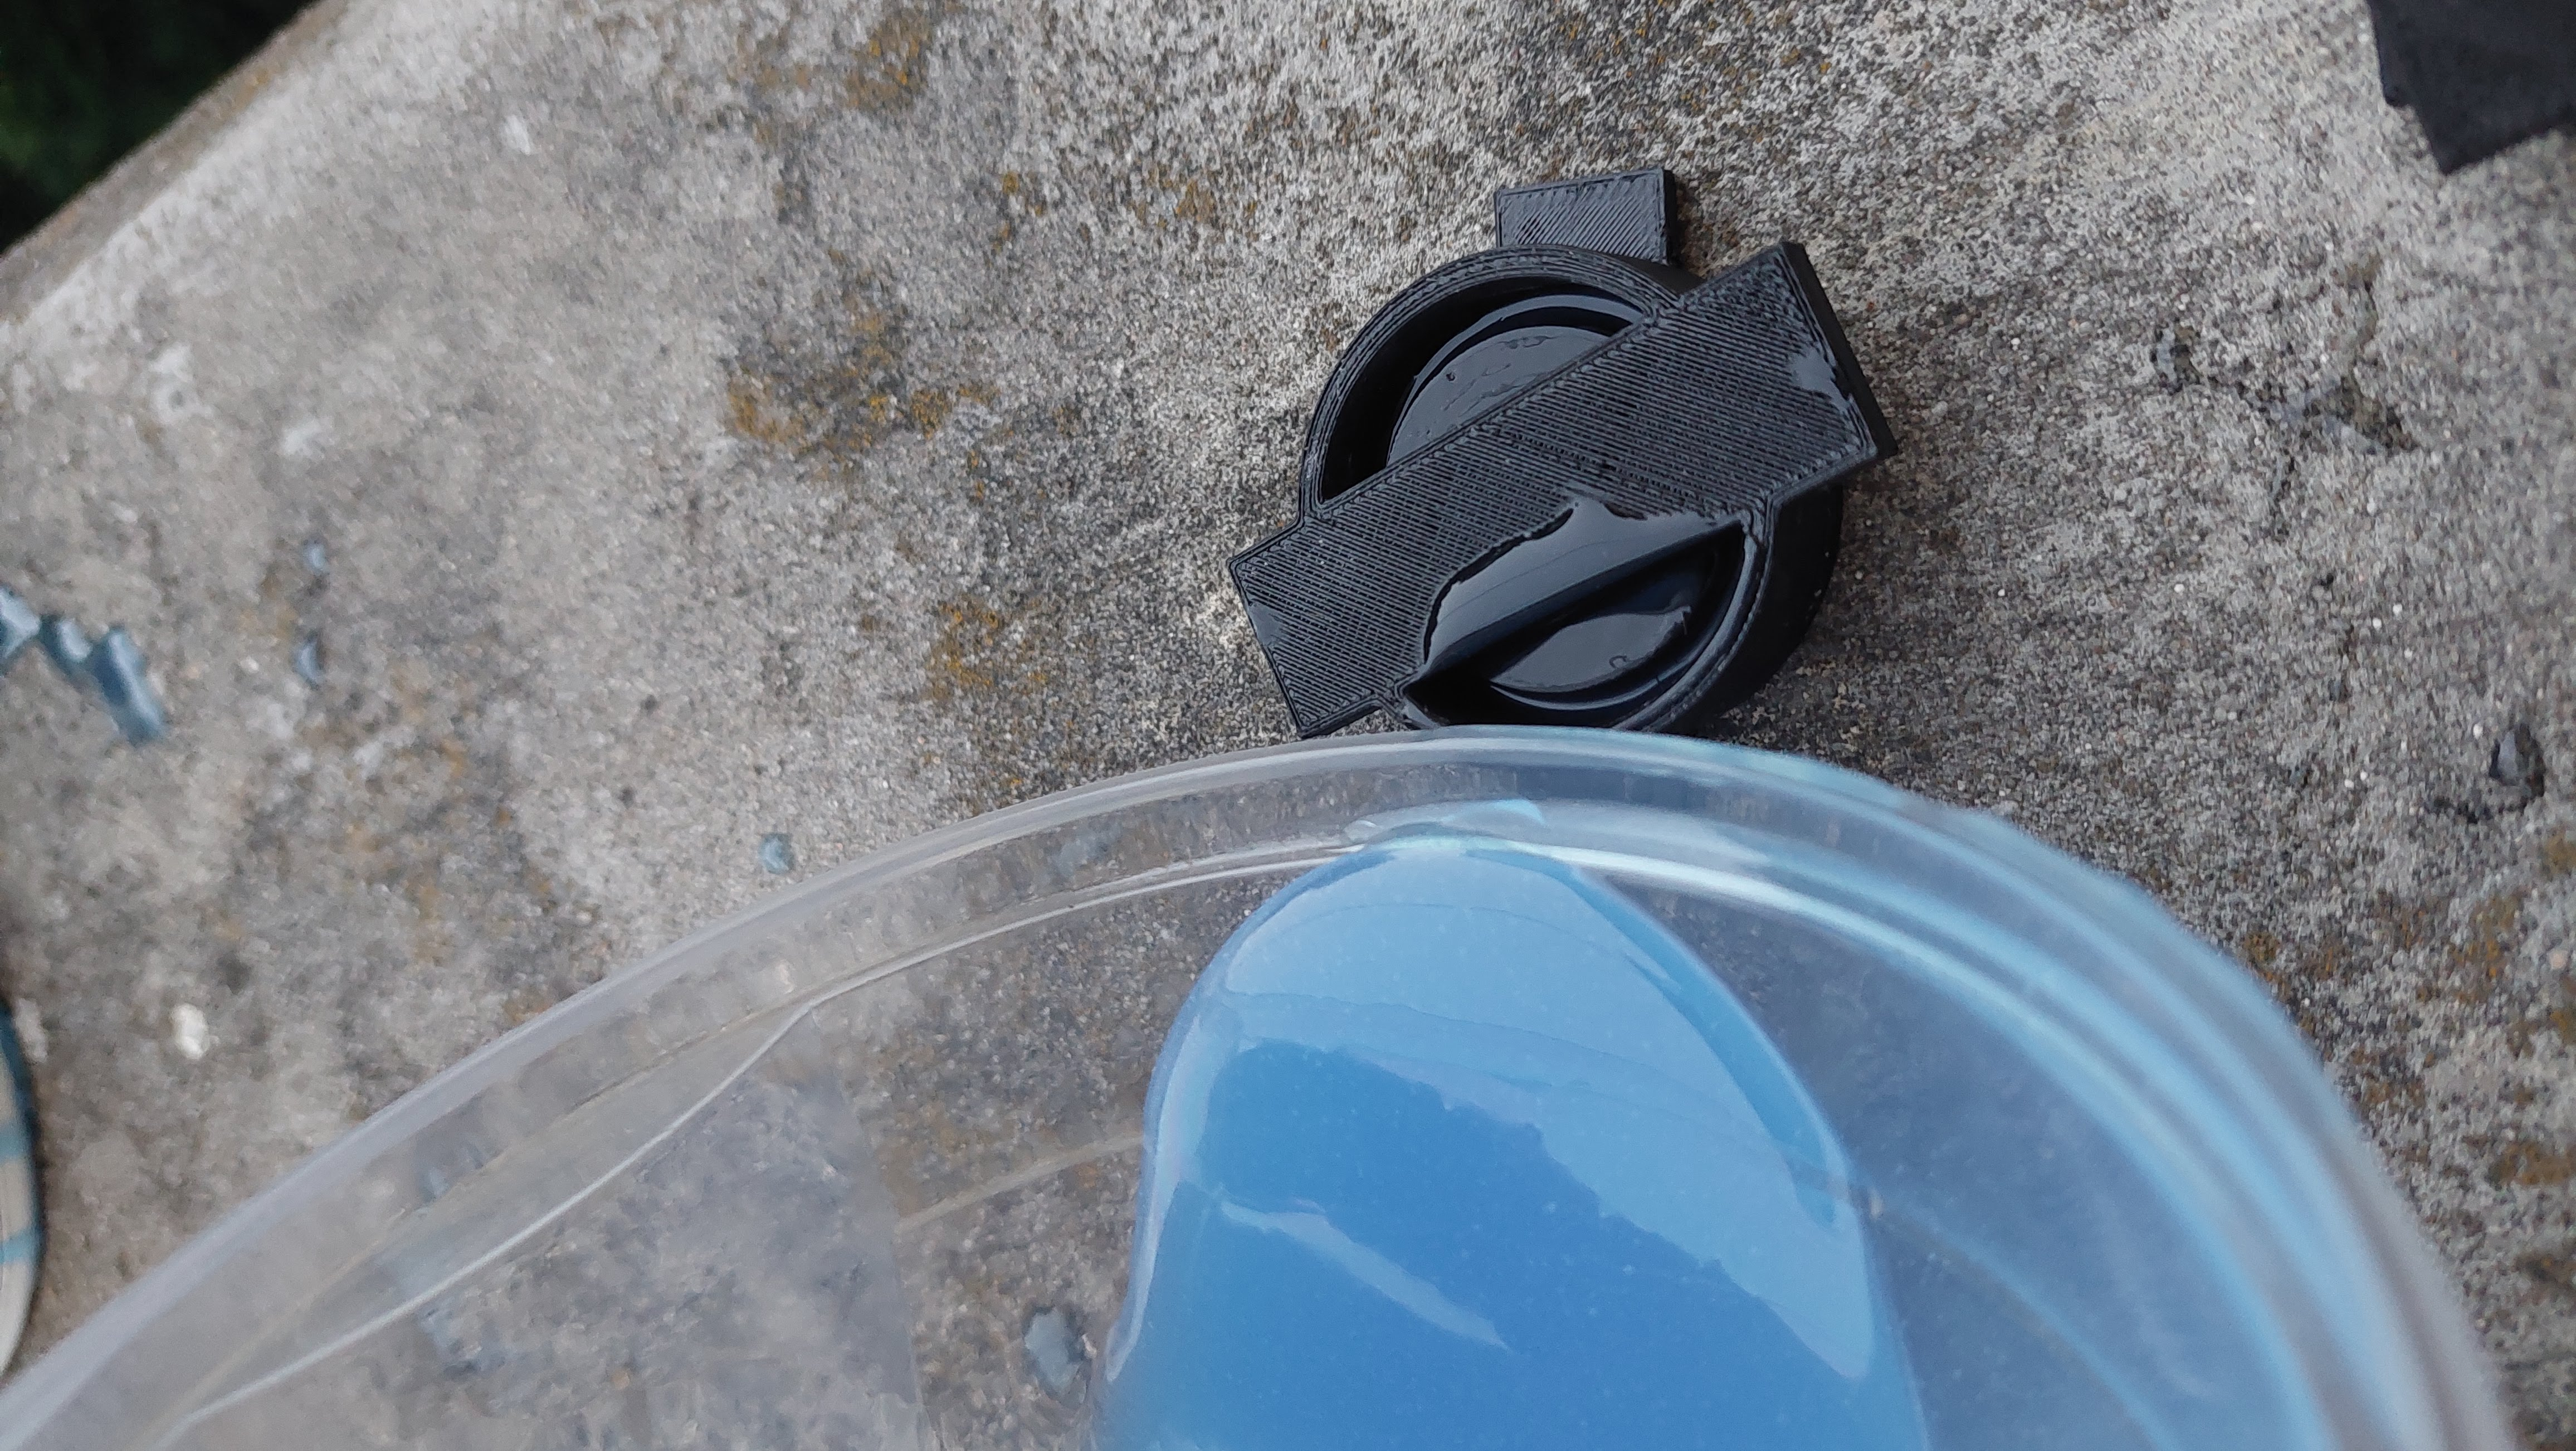
\includegraphics[scale=0.07]{../images/motors/tires_1.jpg}}

\end{frame}


\begin{frame}
  
  \frametitle{\bf making custom silicone tires}
  \url{https://www.kaufland.sk/product/482387287/}

  \centering{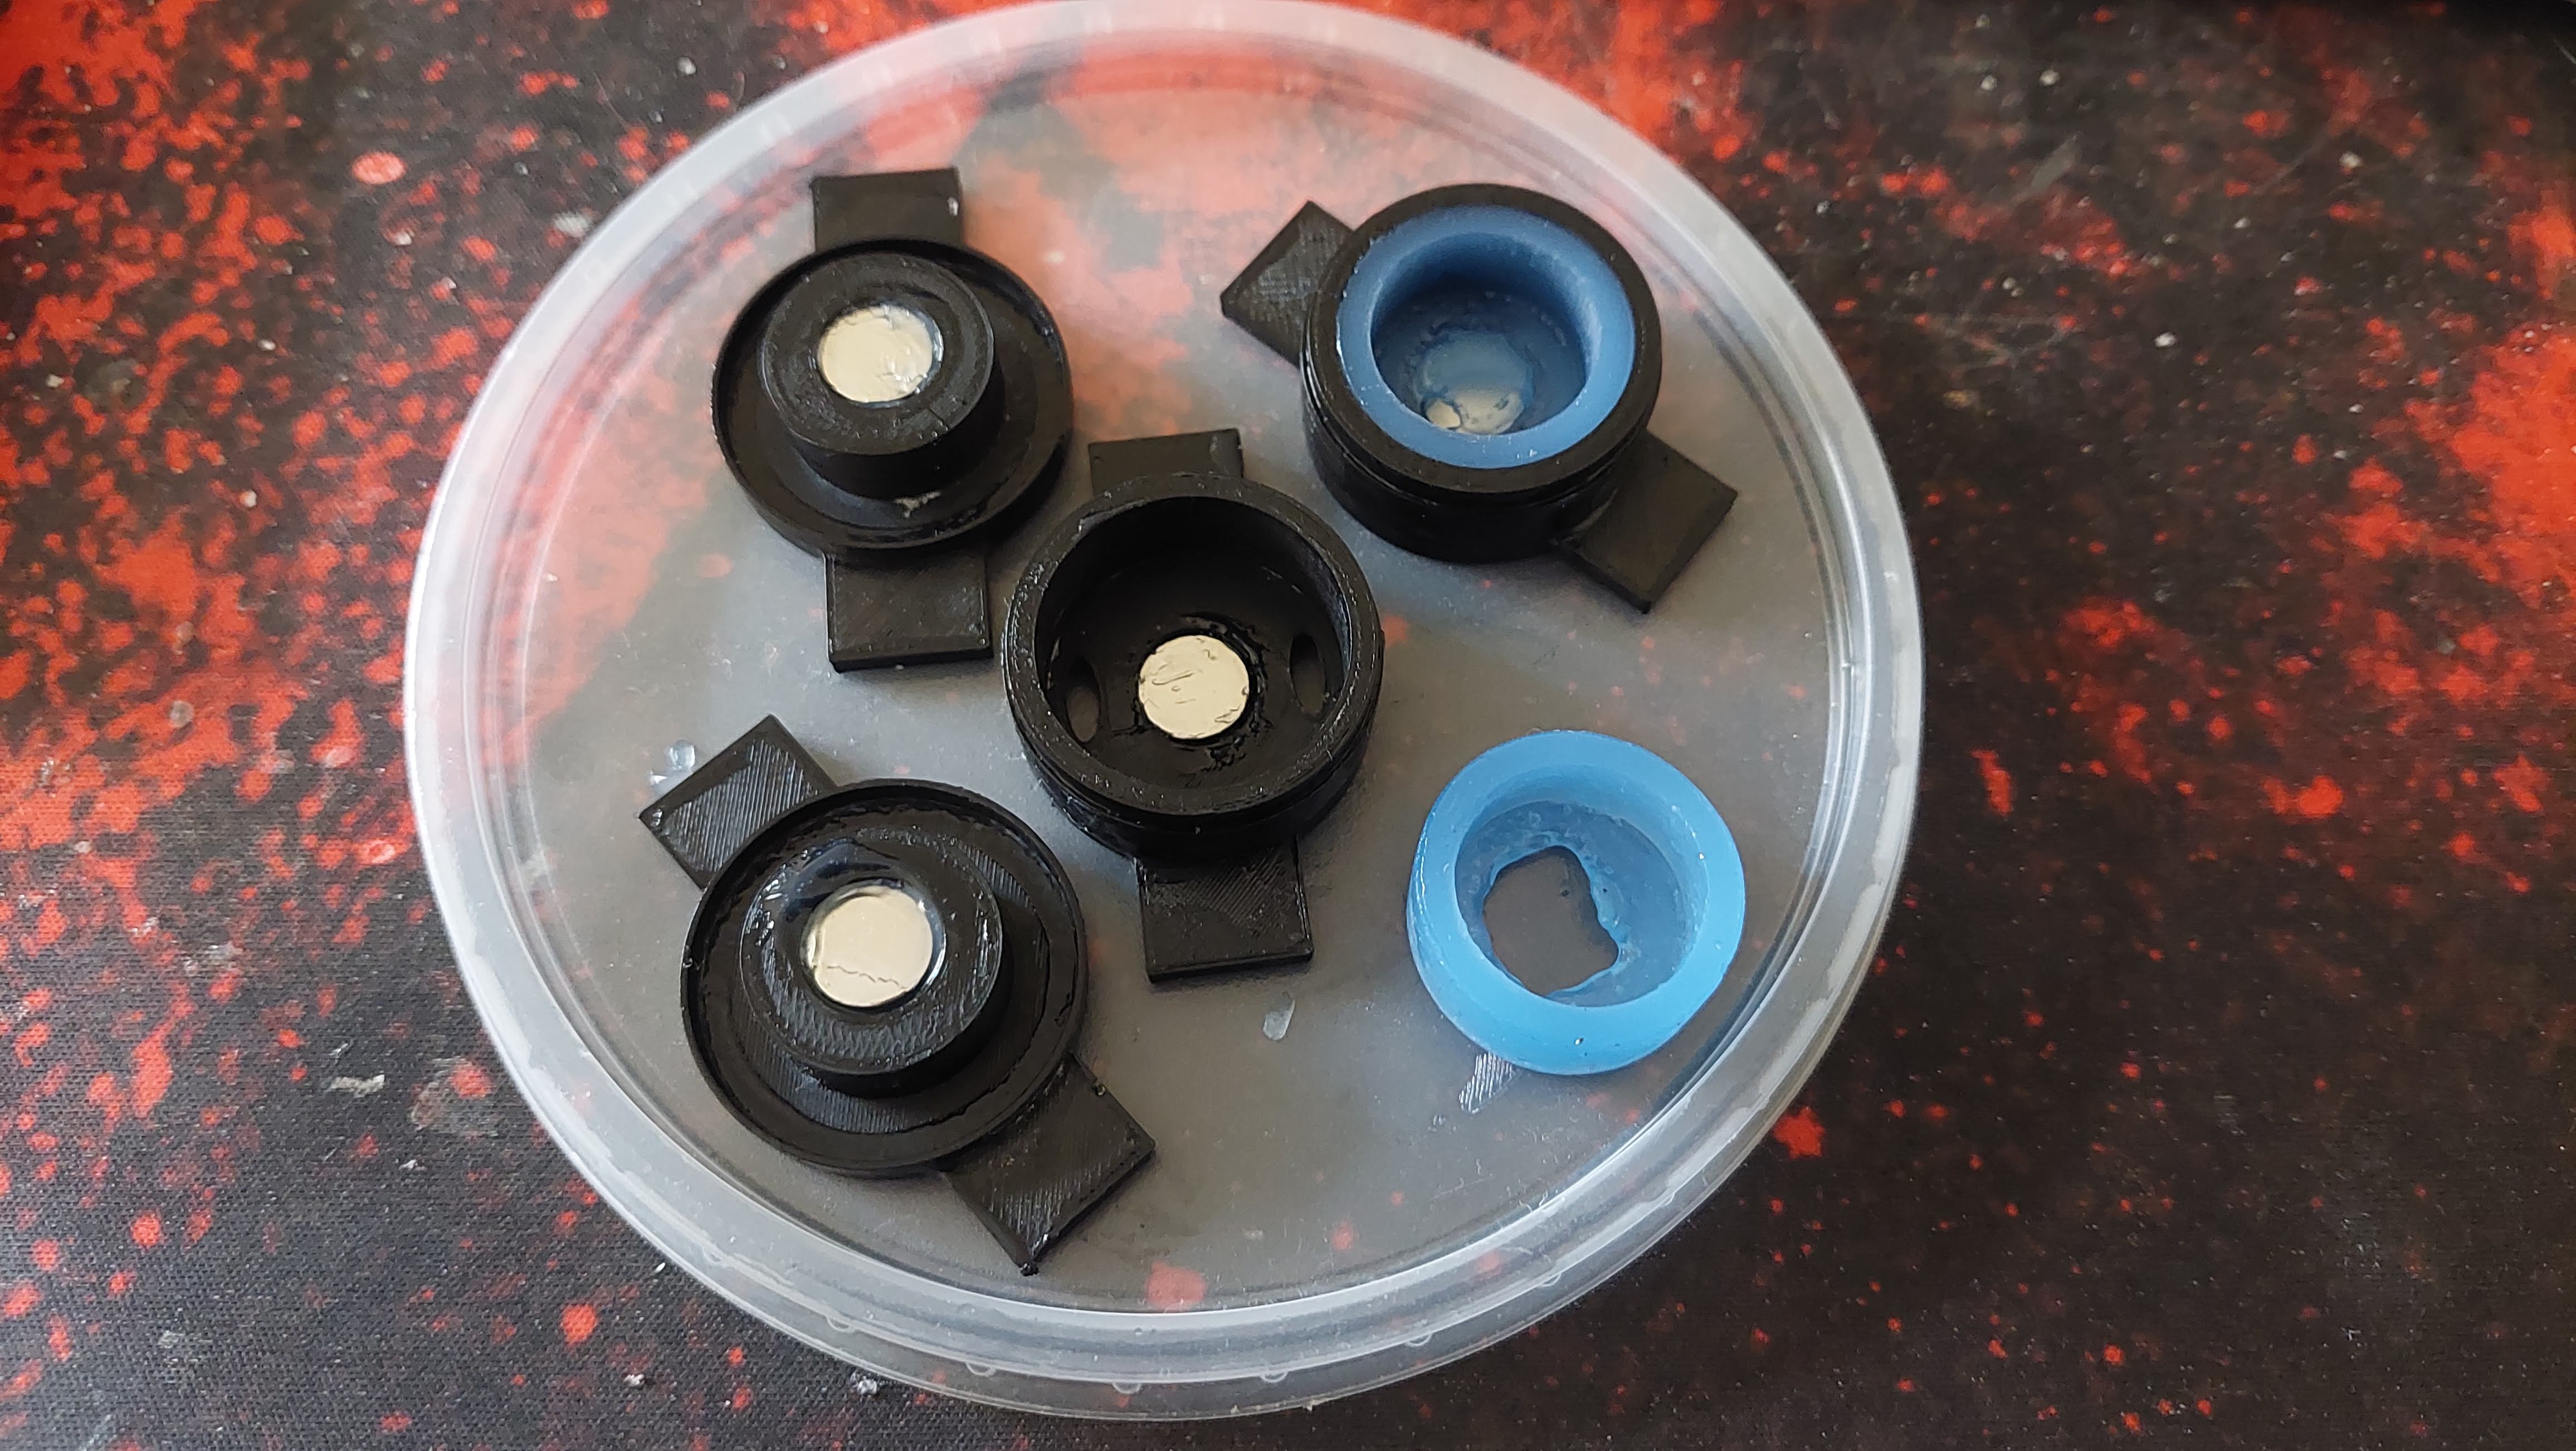
\includegraphics[scale=0.07]{../images/motors/tires_2.jpg}}

\end{frame}

\begin{frame}
  
  \frametitle{\bf making custom silicone tires}
  \url{https://www.kaufland.sk/product/482387287/}

  \centering{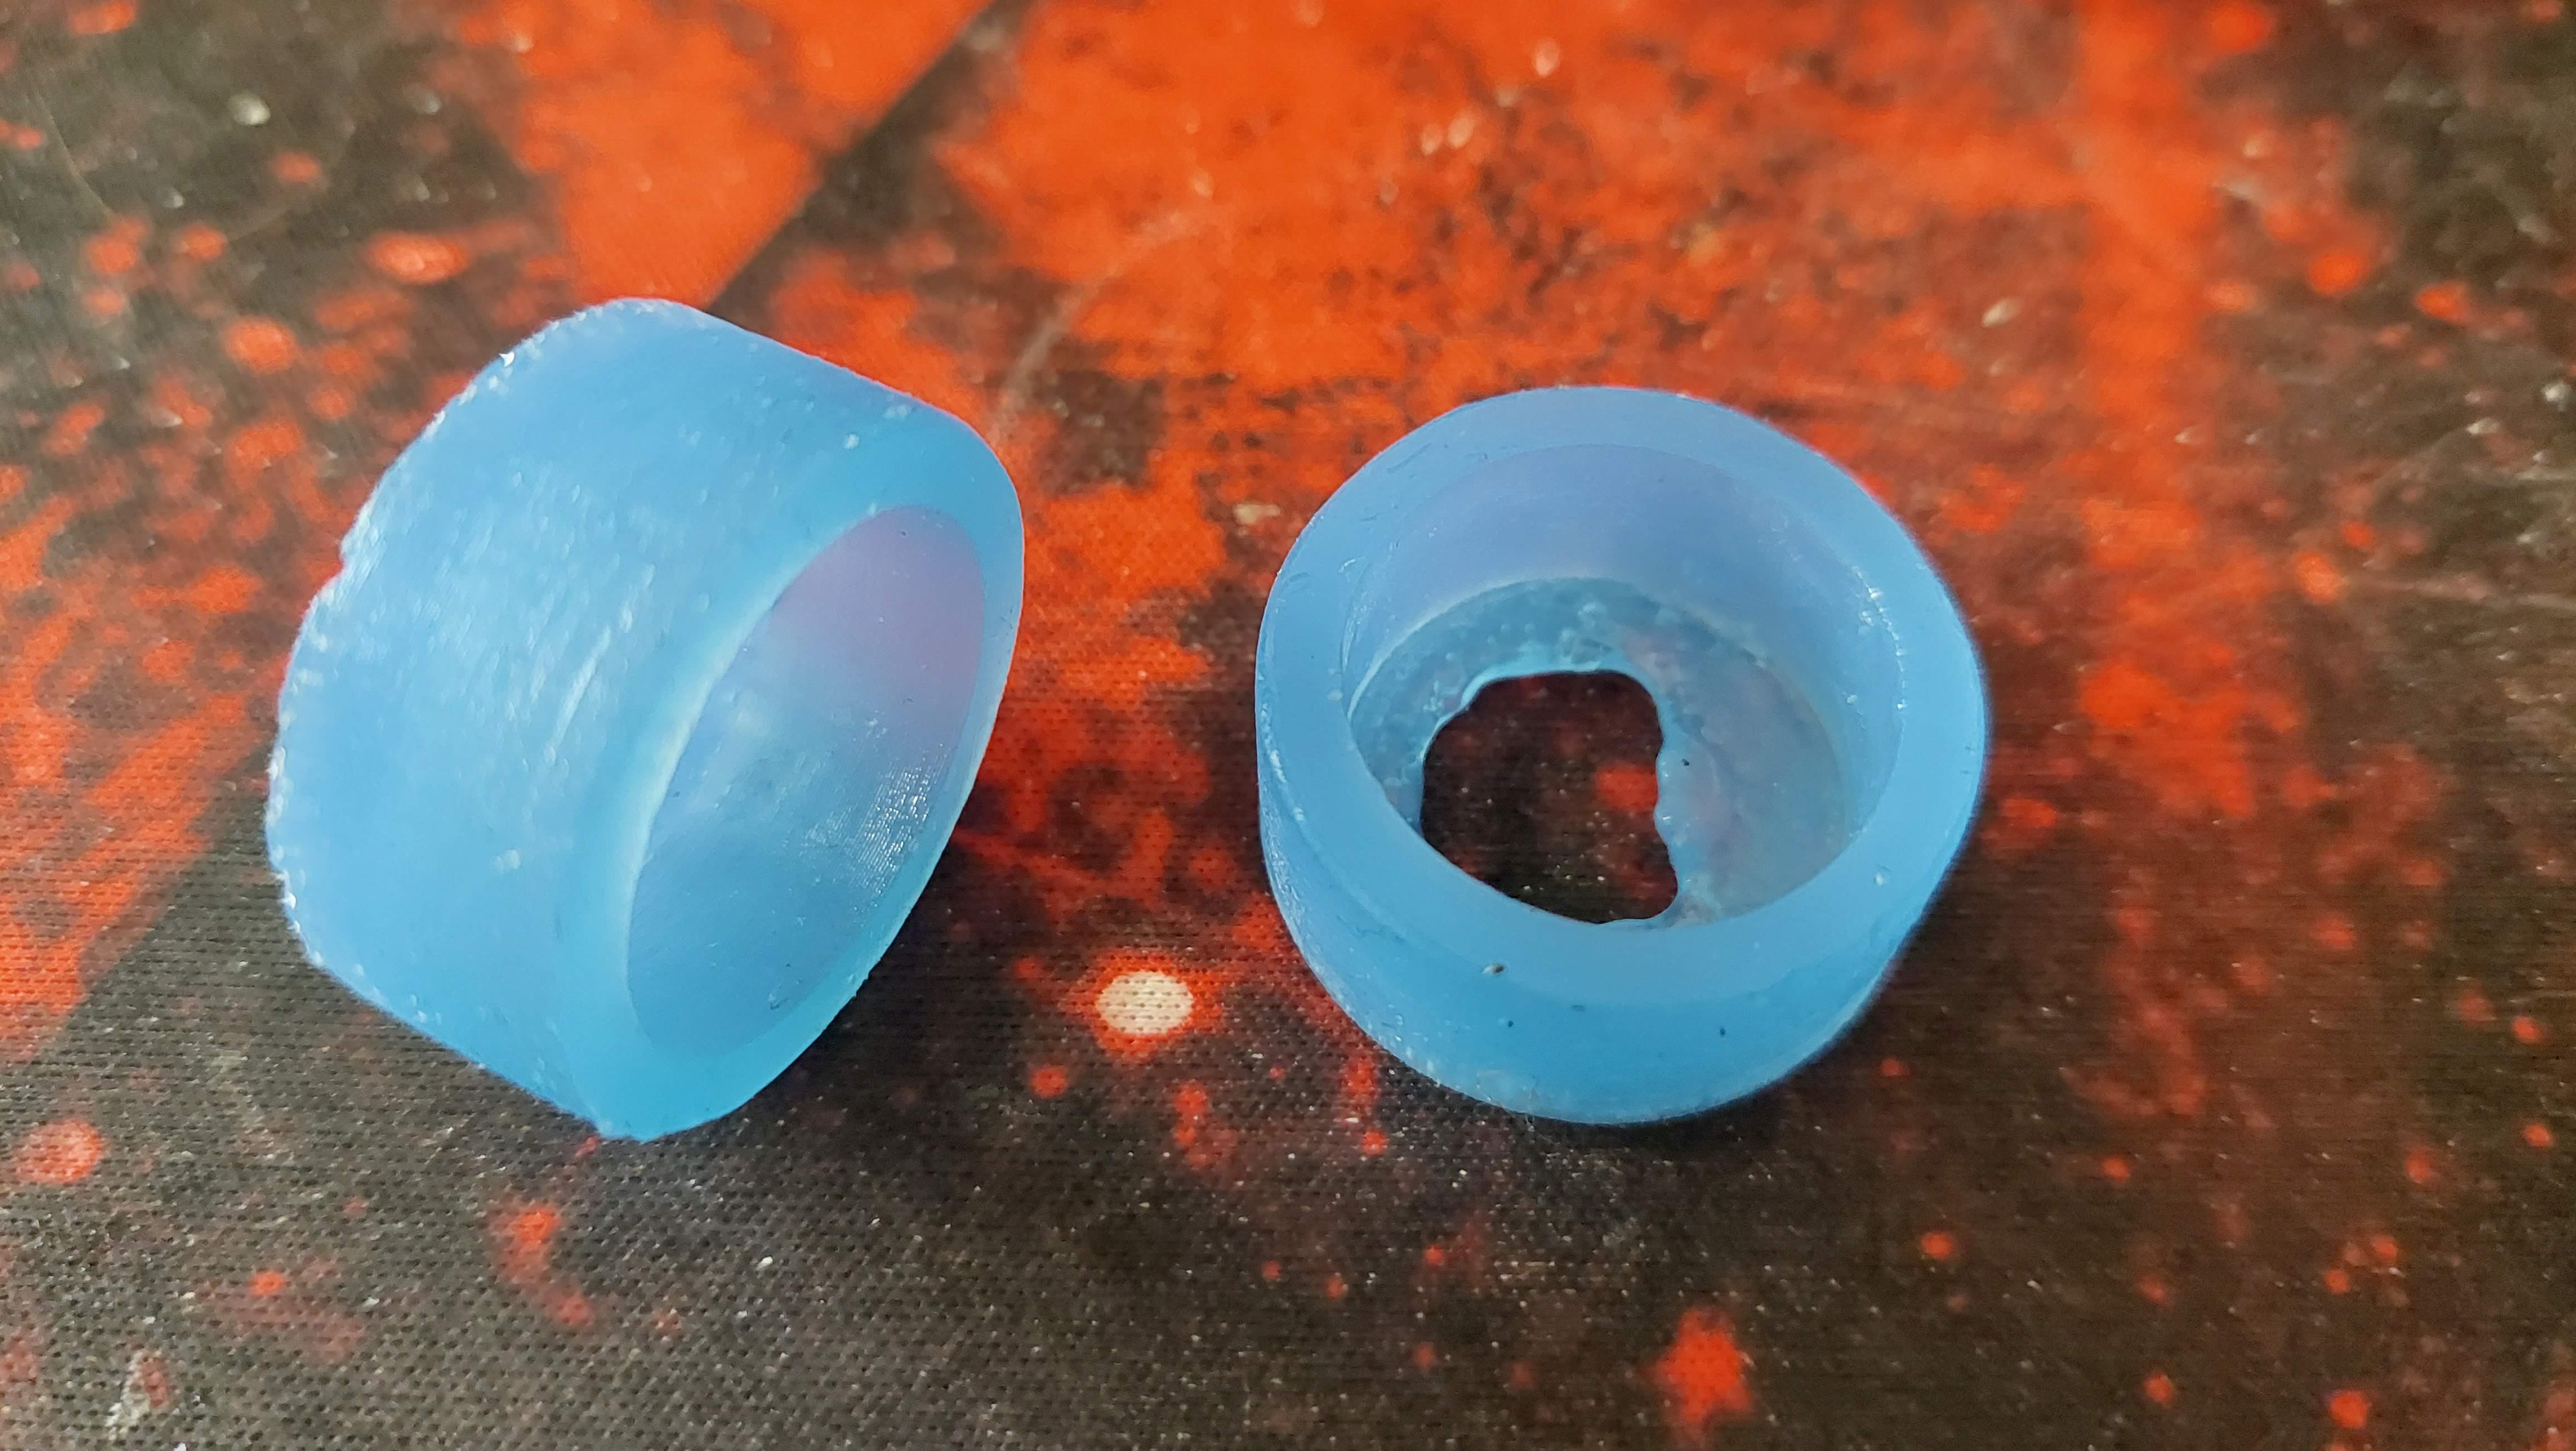
\includegraphics[scale=0.07]{../images/motors/tires_3.jpg}}

\end{frame}





\begin{frame}
  
  \frametitle{\bf sensors}

  \begin{itemize}
    \item line sensors
    \item brick detection
    \item encoders
    \item IMU
  \end{itemize}

\end{frame}


\begin{frame}

  \frametitle{\bf line sensors}
  TODO

\end{frame}



\begin{frame}

  \frametitle{\bf camera}
  
  \begin{columns}

    \begin{column}{0.5\textwidth}
      any DCMI smd camera, e.g. OV2640
      \centering{\includegraphics[scale=0.04]{../images/sensors/camera_1.jpg}}
    \end{column}

    \begin{column}{0.5\textwidth}
      line scan camera, TSL1401CL, 128pixels, analog out
      \centering{\includegraphics[scale=0.04]{../images/sensors/camera_2.jpg}}
    \end{column}

   
  \end{columns}

\end{frame}



\begin{frame}

  \frametitle{\bf IR leds sensors}
  TODO

\end{frame}


\begin{frame}
  
  \frametitle{\bf laser TOF}

  {\color{red} \bf{ NEVER } buy cheep alternative}

  \centering{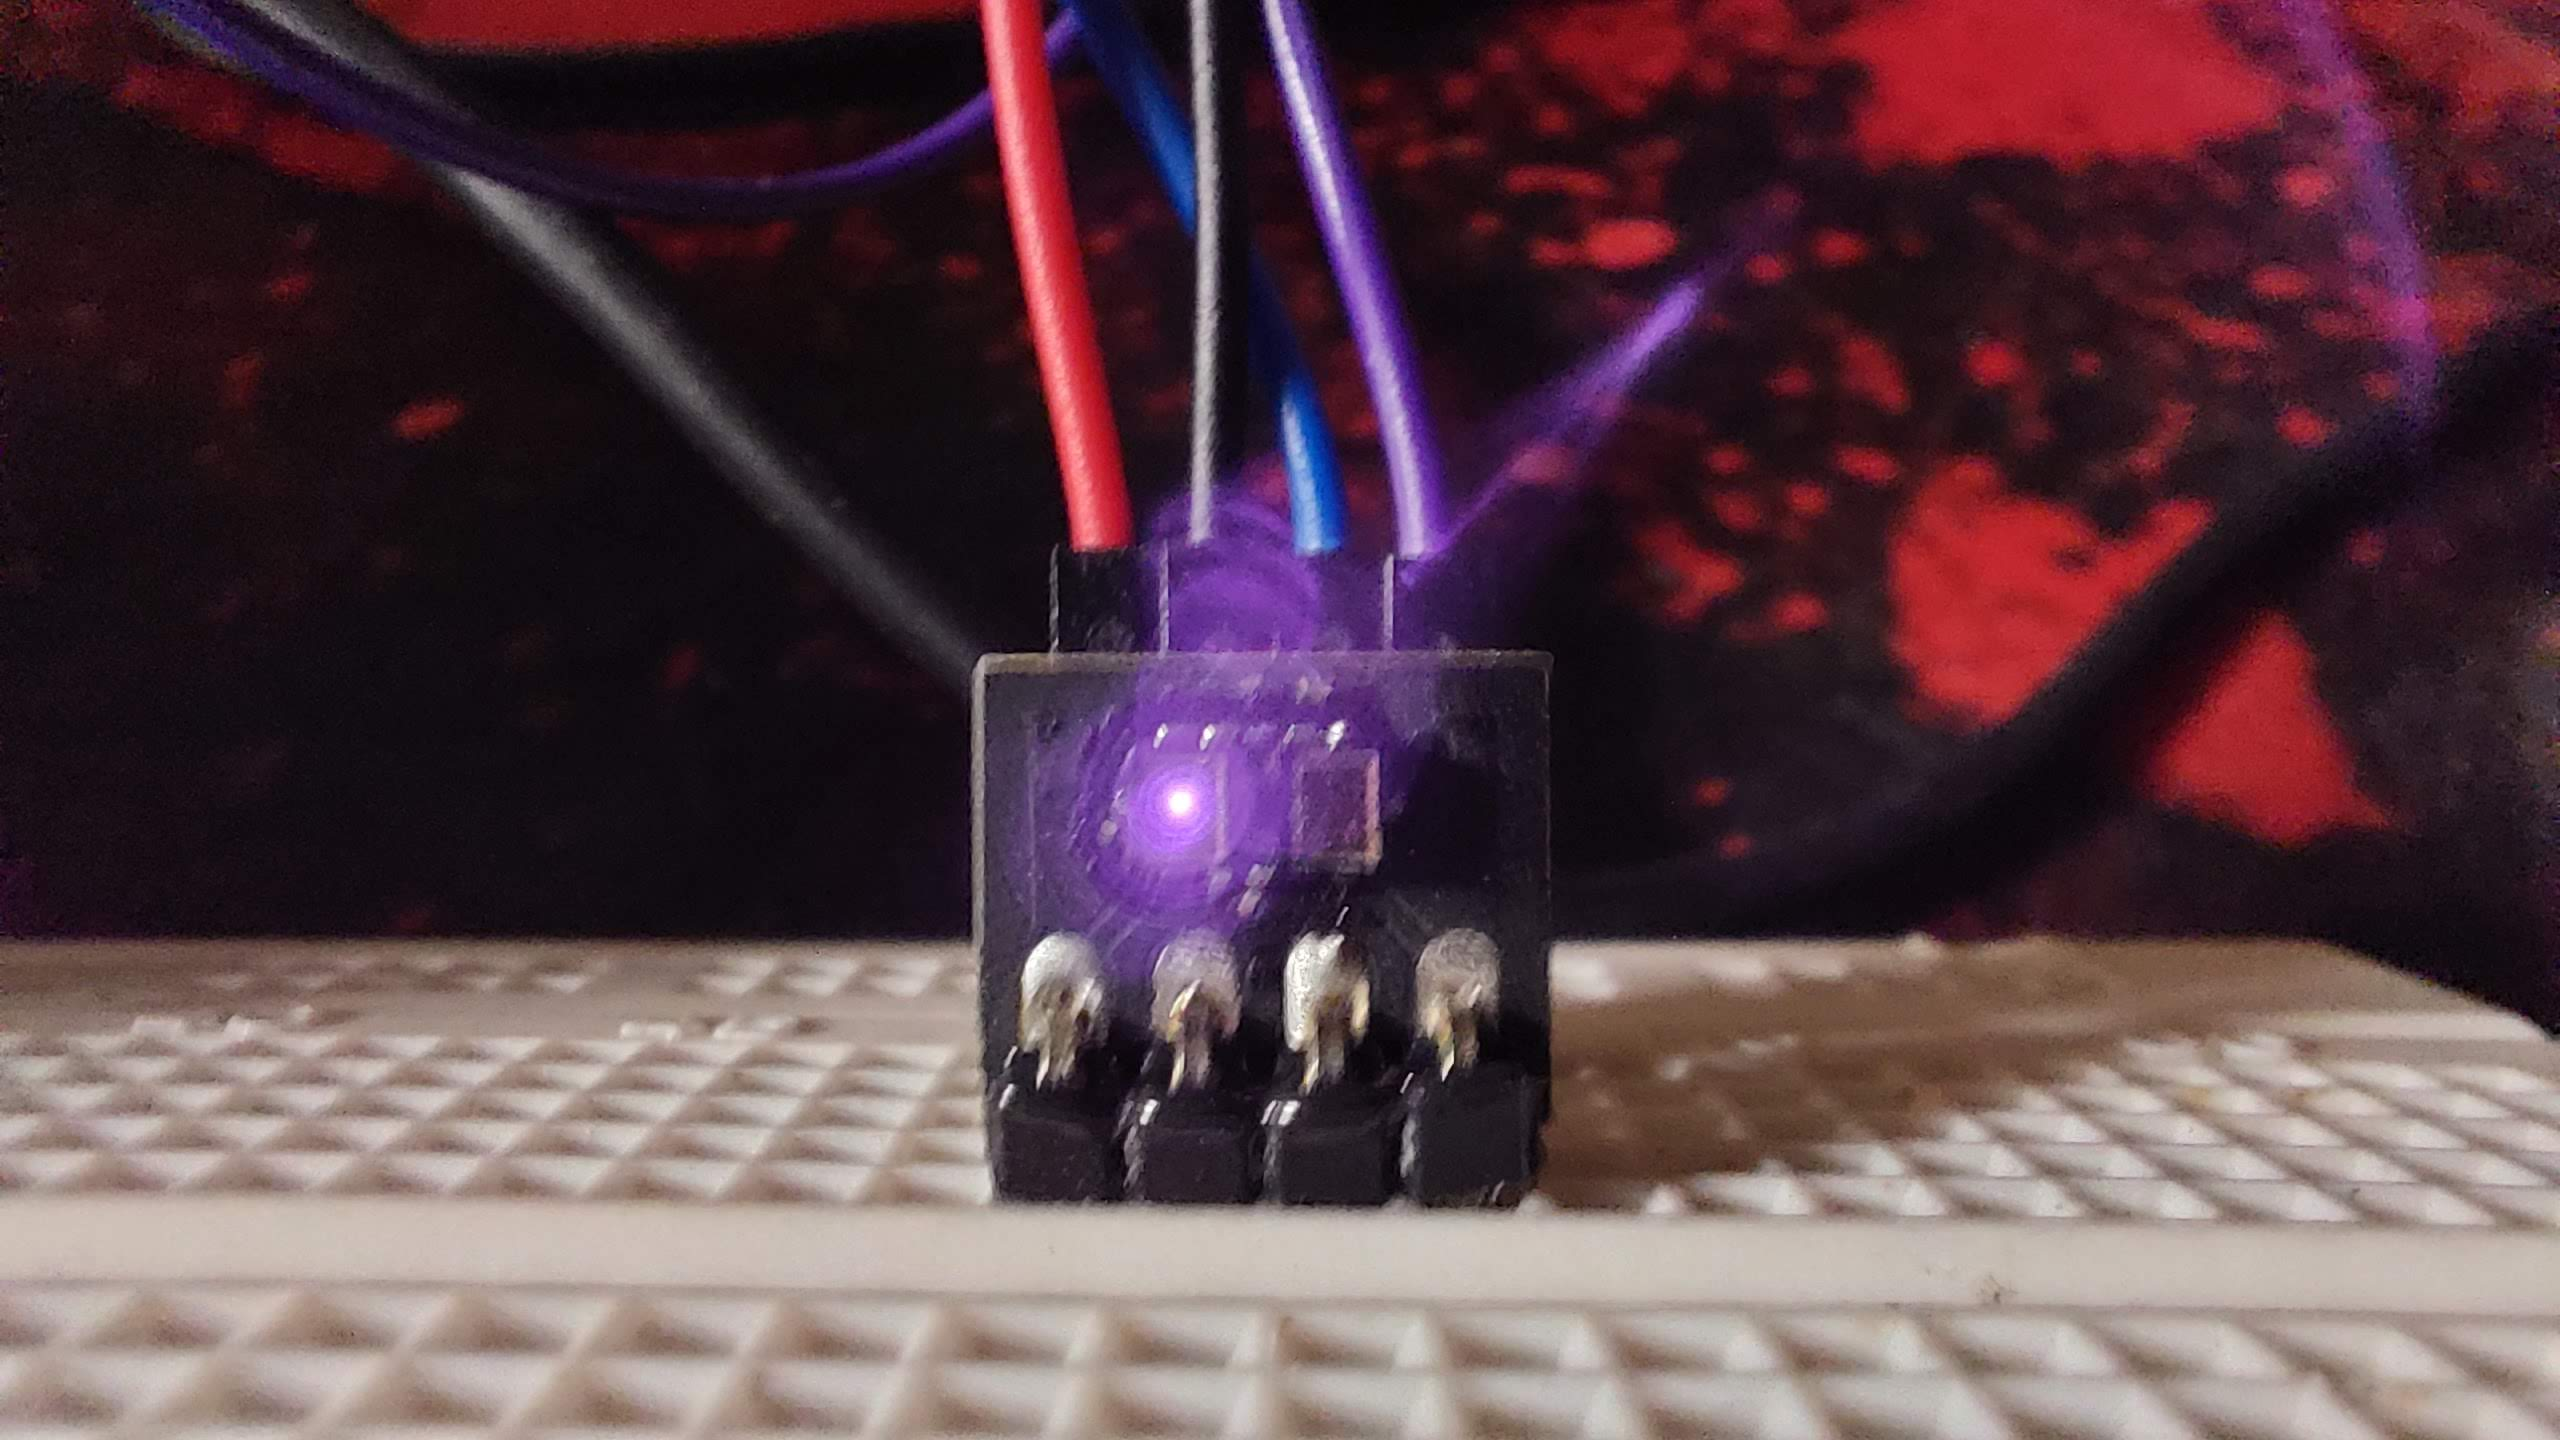
\includegraphics[scale=0.08]{../images/sensors/tof_1.jpg}}
  \centering{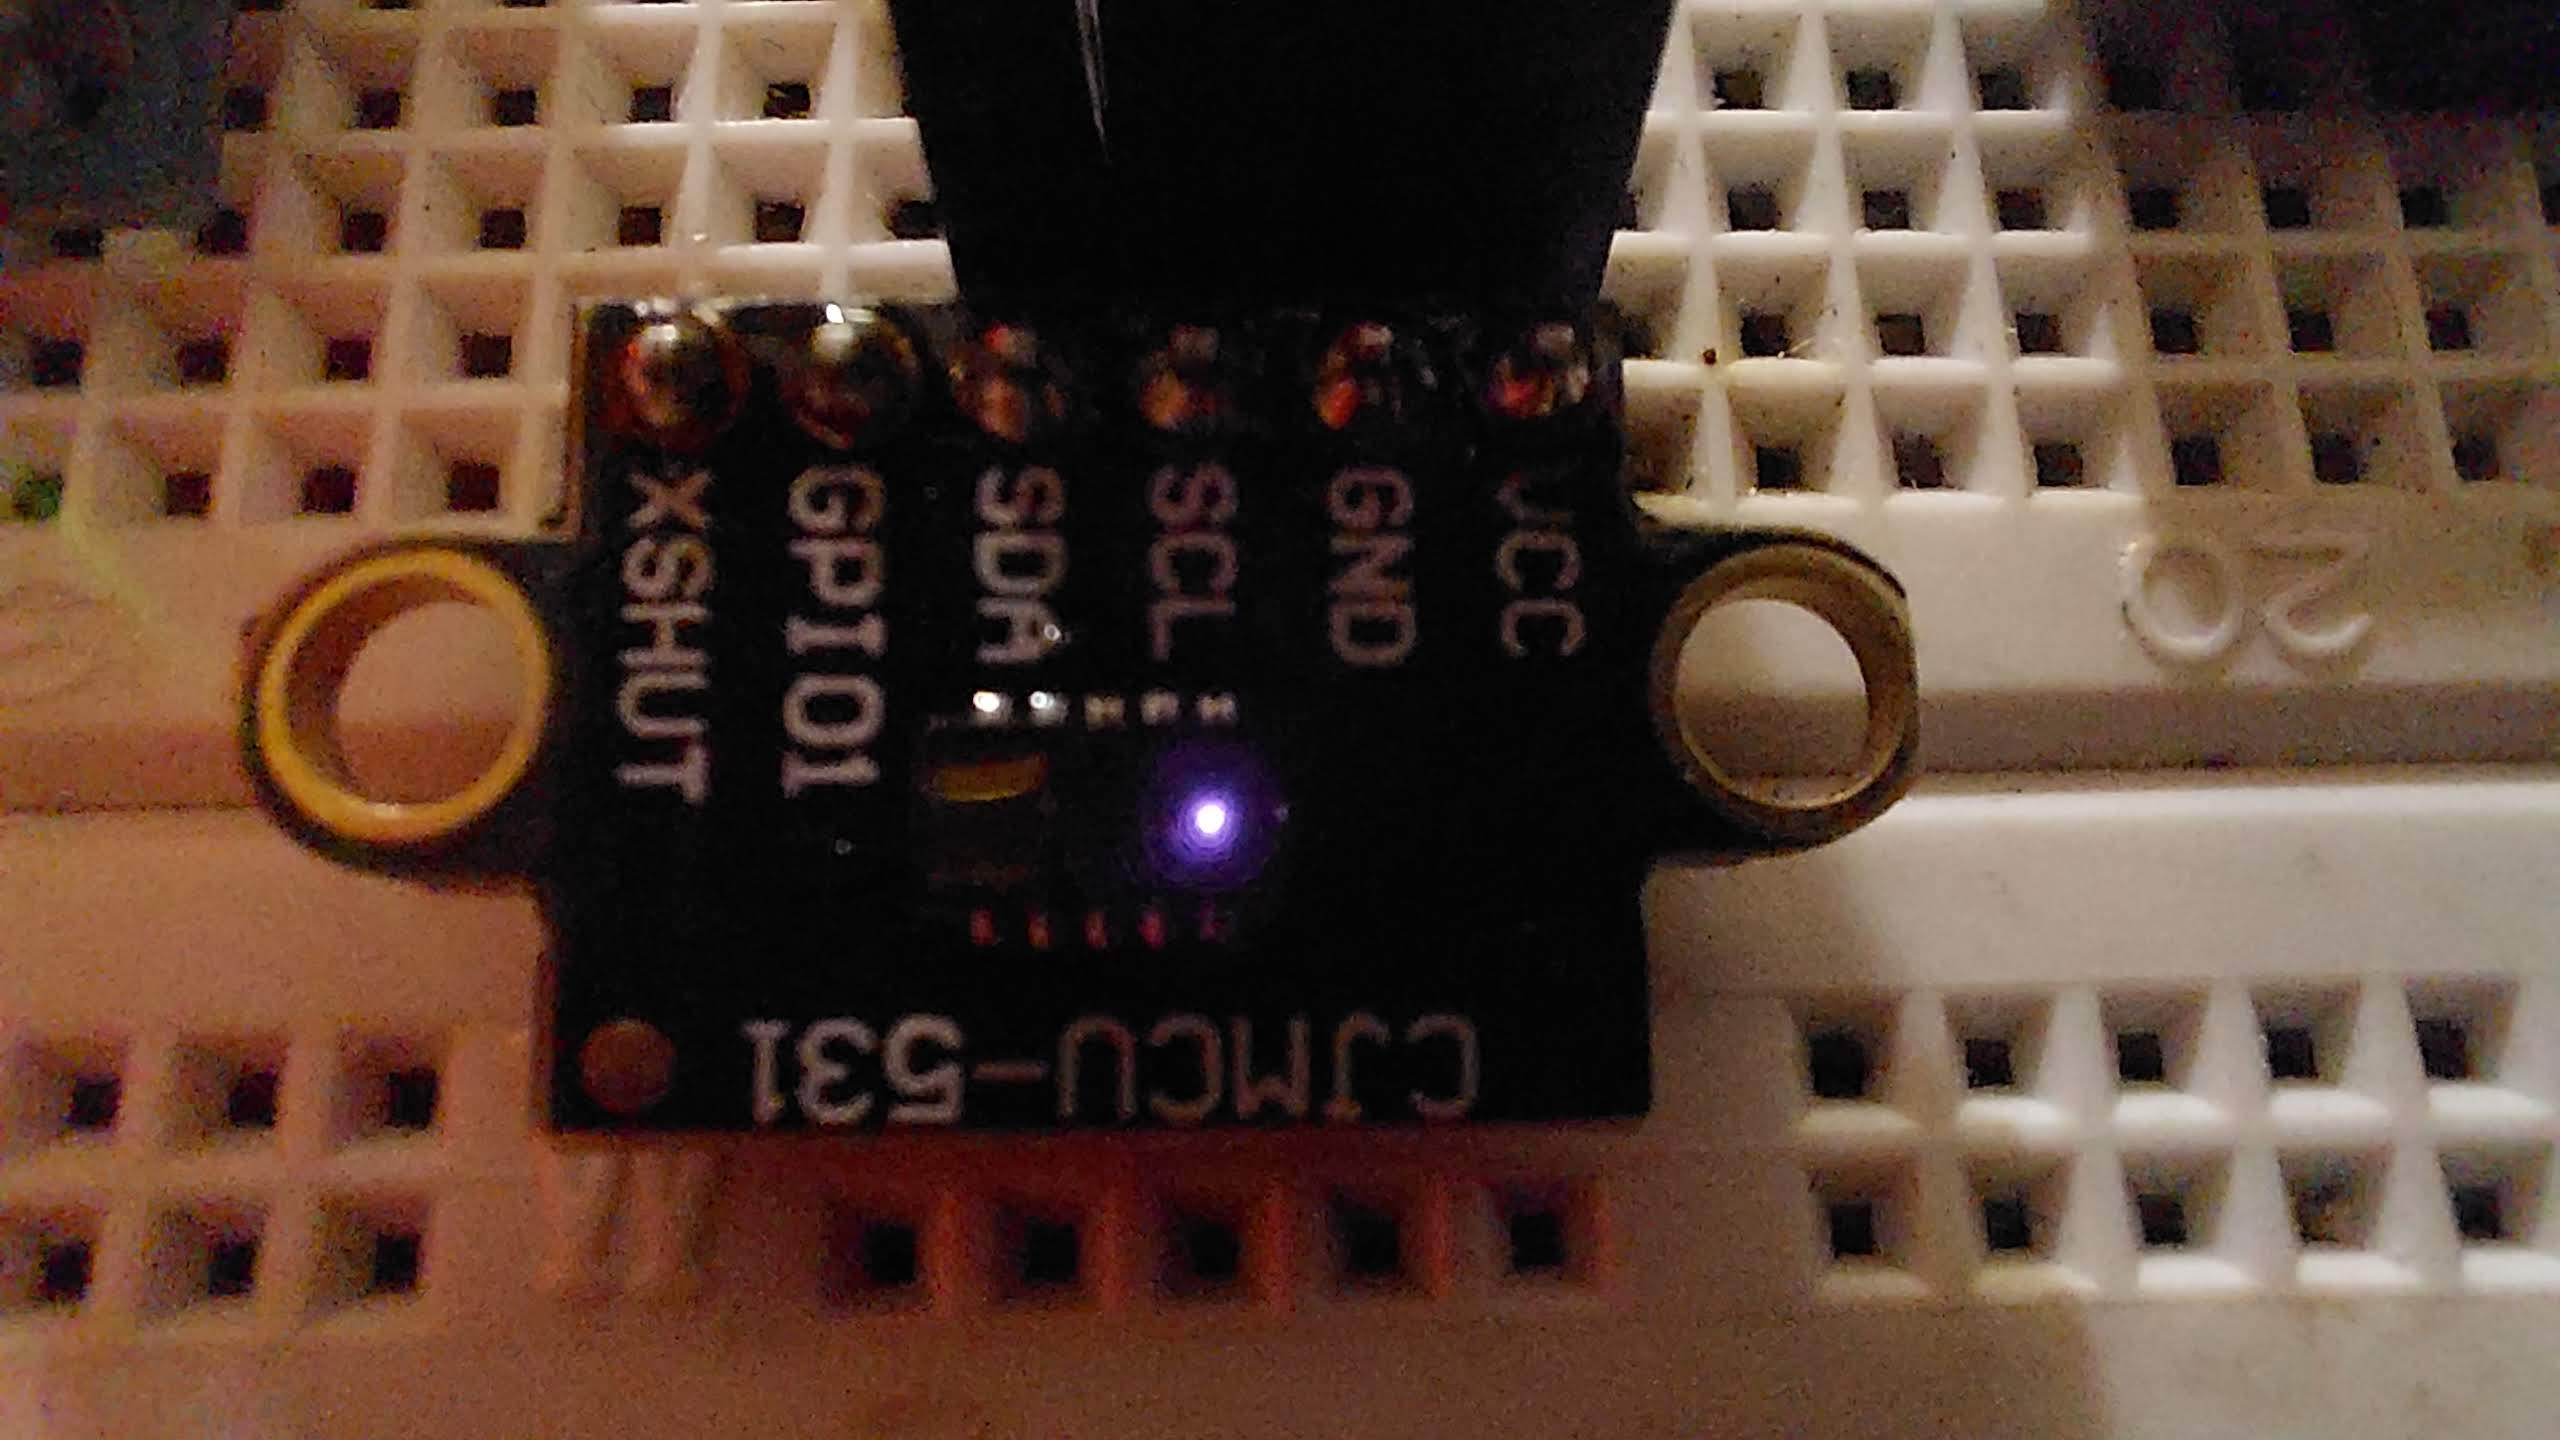
\includegraphics[scale=0.08]{../images/sensors/tof_2.jpg}}
  

\end{frame}


\begin{frame}
  
  \frametitle{\bf laser TOF - filter data}

  \centering{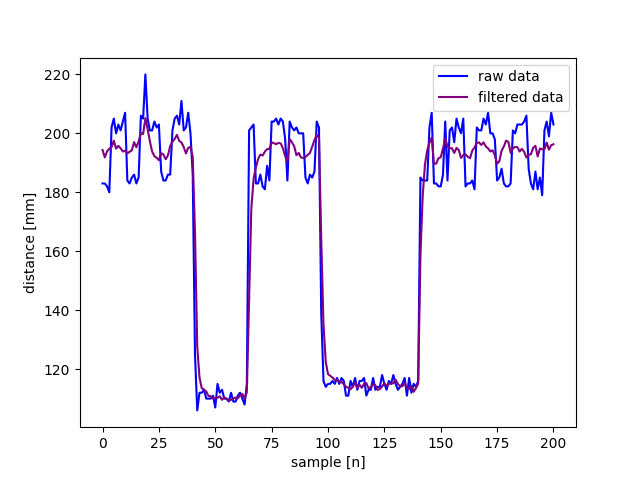
\includegraphics[scale=0.4]{../images/sensors/vl_01.png}}

\end{frame}


\begin{frame}
  
  \frametitle{\bf laser}

  \centering{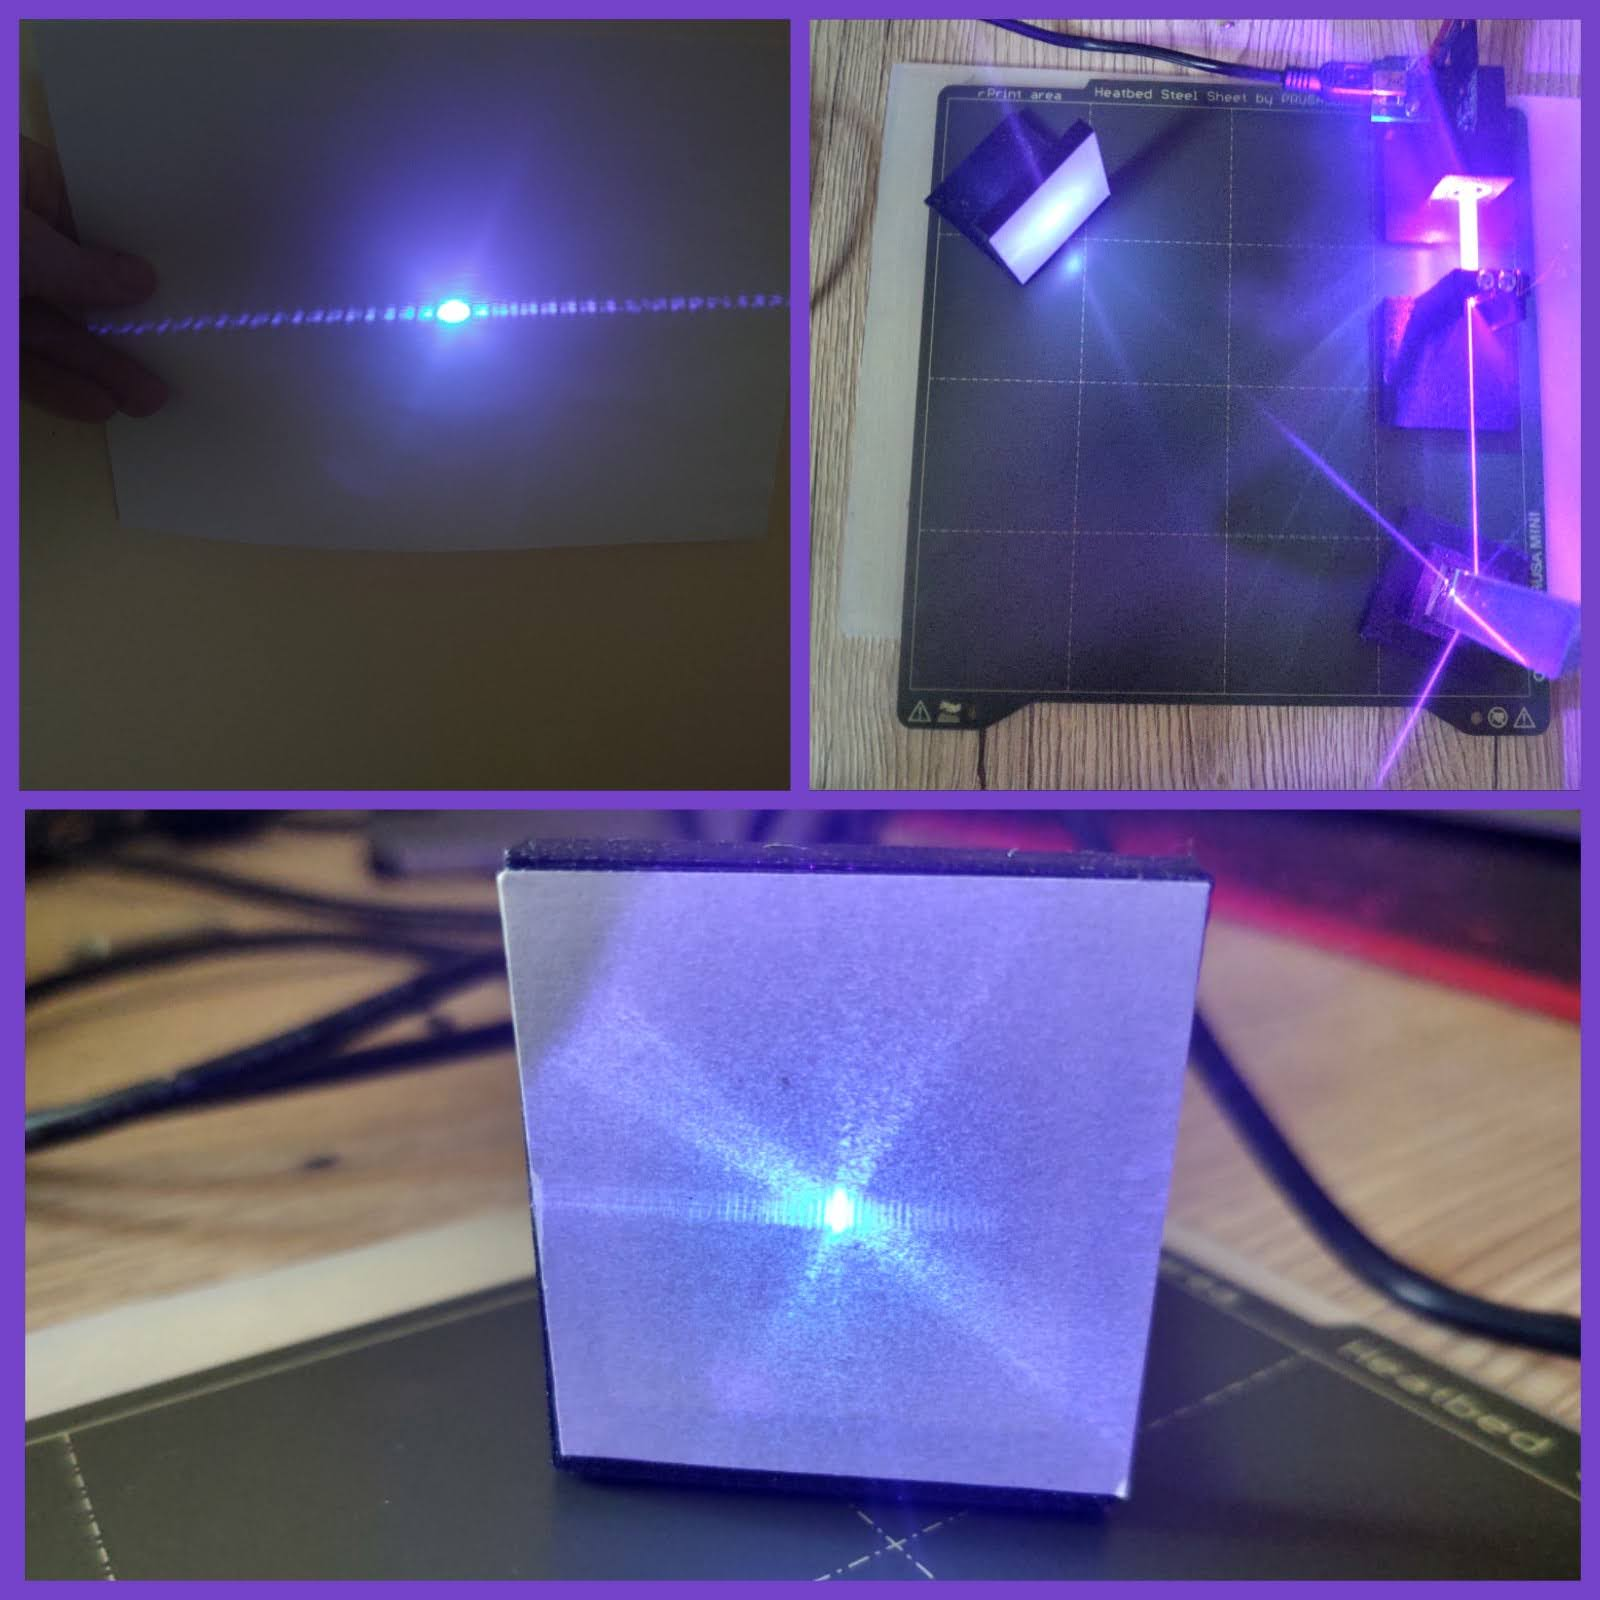
\includegraphics[scale=0.17]{../images/sensors/laser.jpg}}

\end{frame}


\begin{frame}

  \frametitle{\bf encoders}
  TODO

\end{frame}



\begin{frame}
  \frametitle{\bf robot controll}

  control levels :
  \begin{itemize}
    \item commutation loop : 4kHz, fixed point arithmetics
    \item velocity  loop   : 1..4kHz, PI or simple LQR controller
    \item position loop    : 100..500Hz, LQR or MPC controller
    \item planning loop    : 10..20Hz, MPC or neural network
  \end{itemize}

  building blocks :
  \begin{itemize}
    \item if else : never captures dynamics
    \item PID     : only SISO systems, only hand tunning
    \item LQR+Kalman filter : MIMO systems, exact solution
    \item MPC : MIMO systems, tracking (planning trajectory)
    \item neural network :RNN (LSTM or GRU), reinforcement learning
  \end{itemize}

\end{frame}


  

\begin{frame}
  
  \frametitle{\bf robot controll - overview}

  \centering{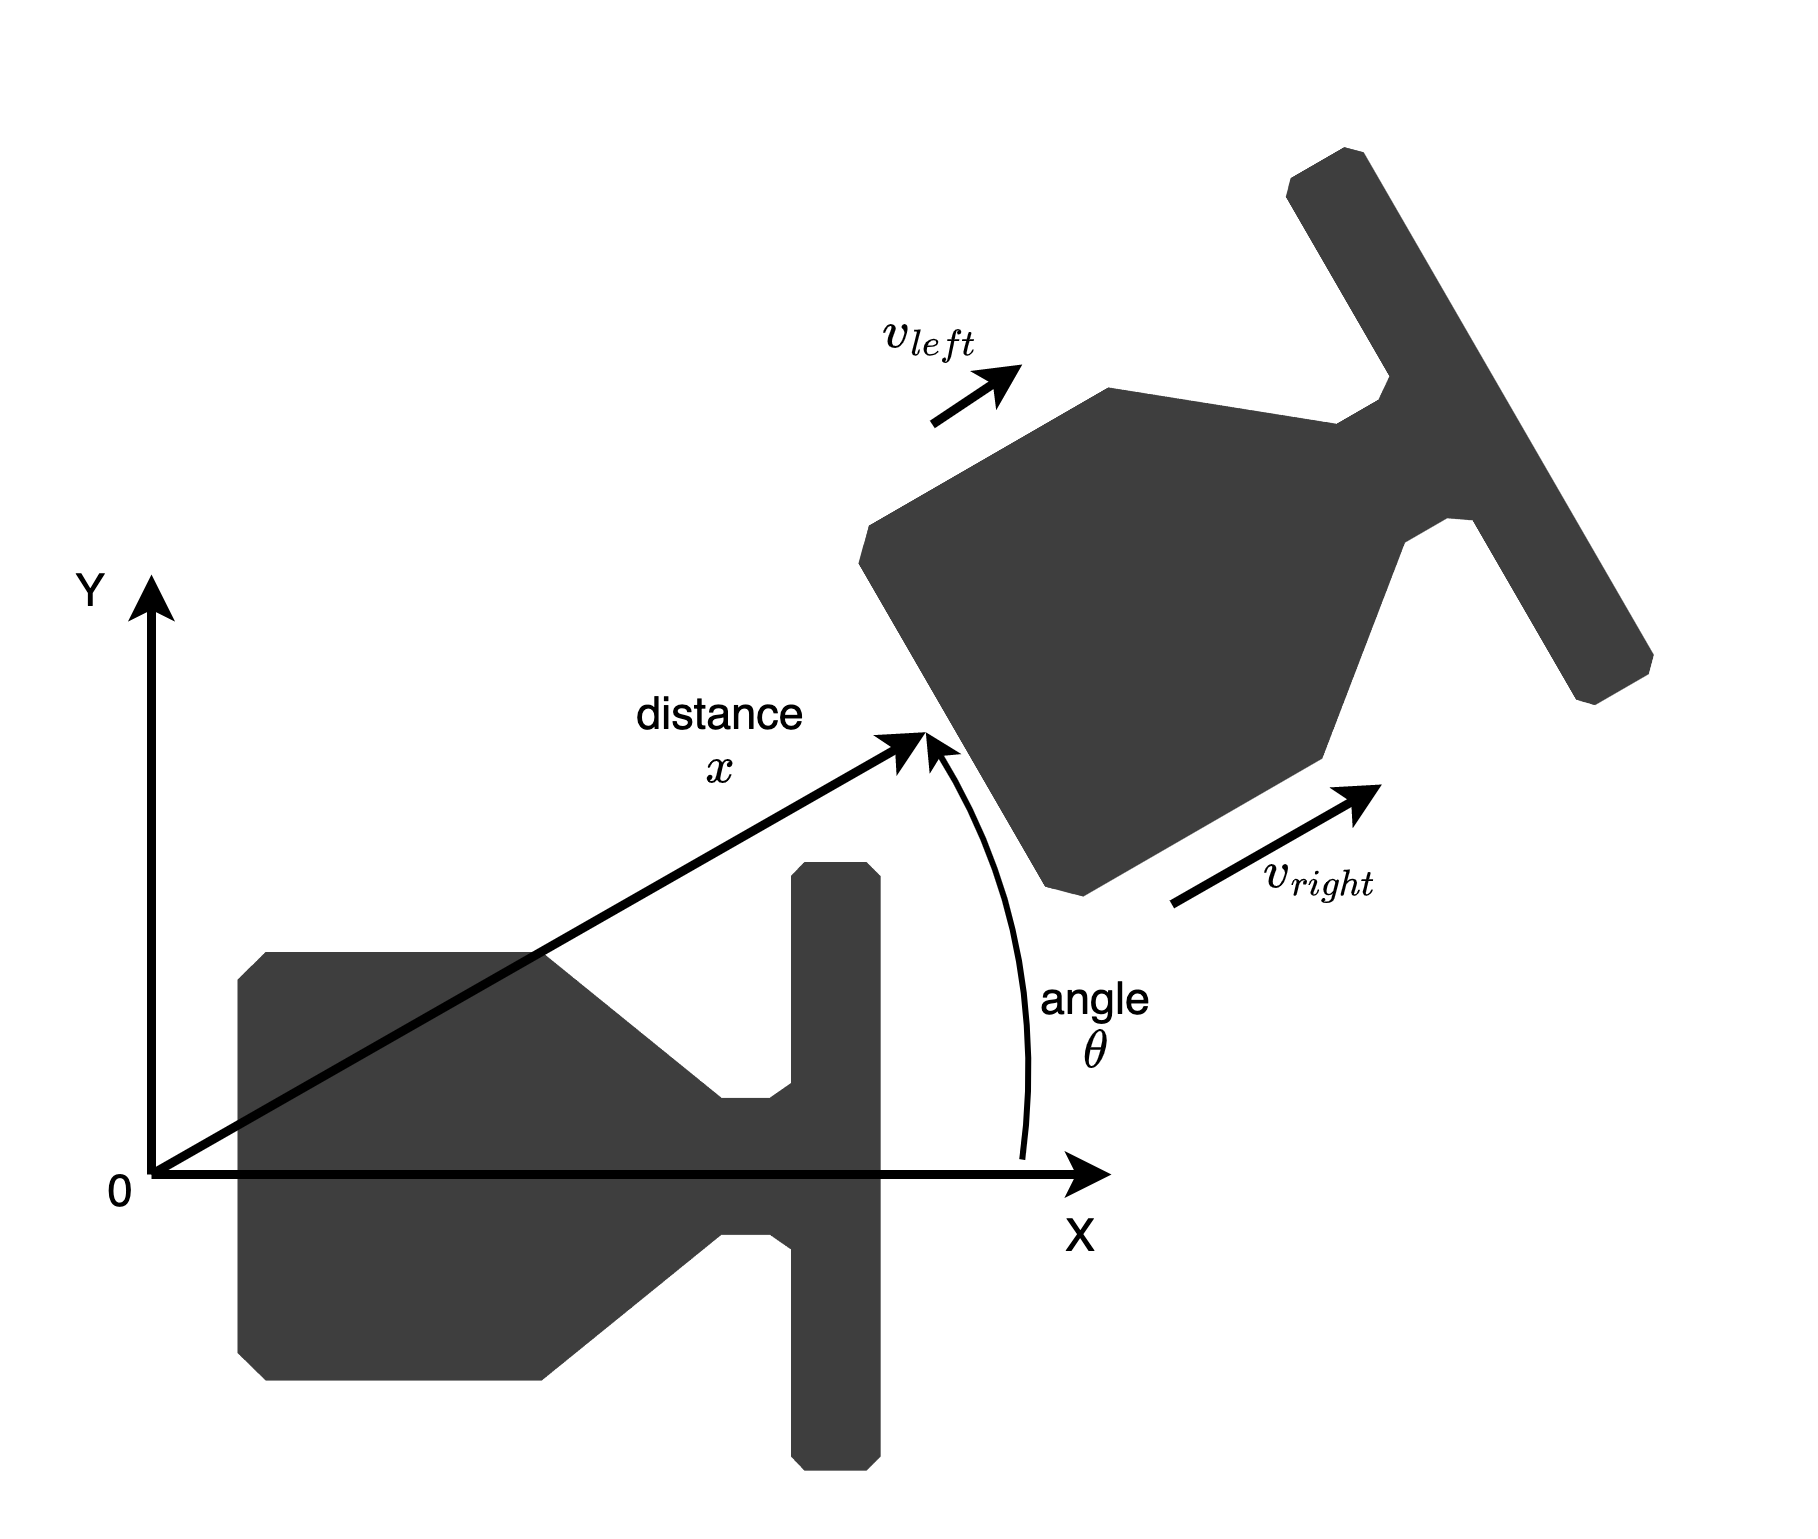
\includegraphics[scale=0.4]{../diagrams/robot_control/control-movement.png}}

\end{frame}


\begin{frame}
  
  \frametitle{\bf robot controll - translation}

  \centering{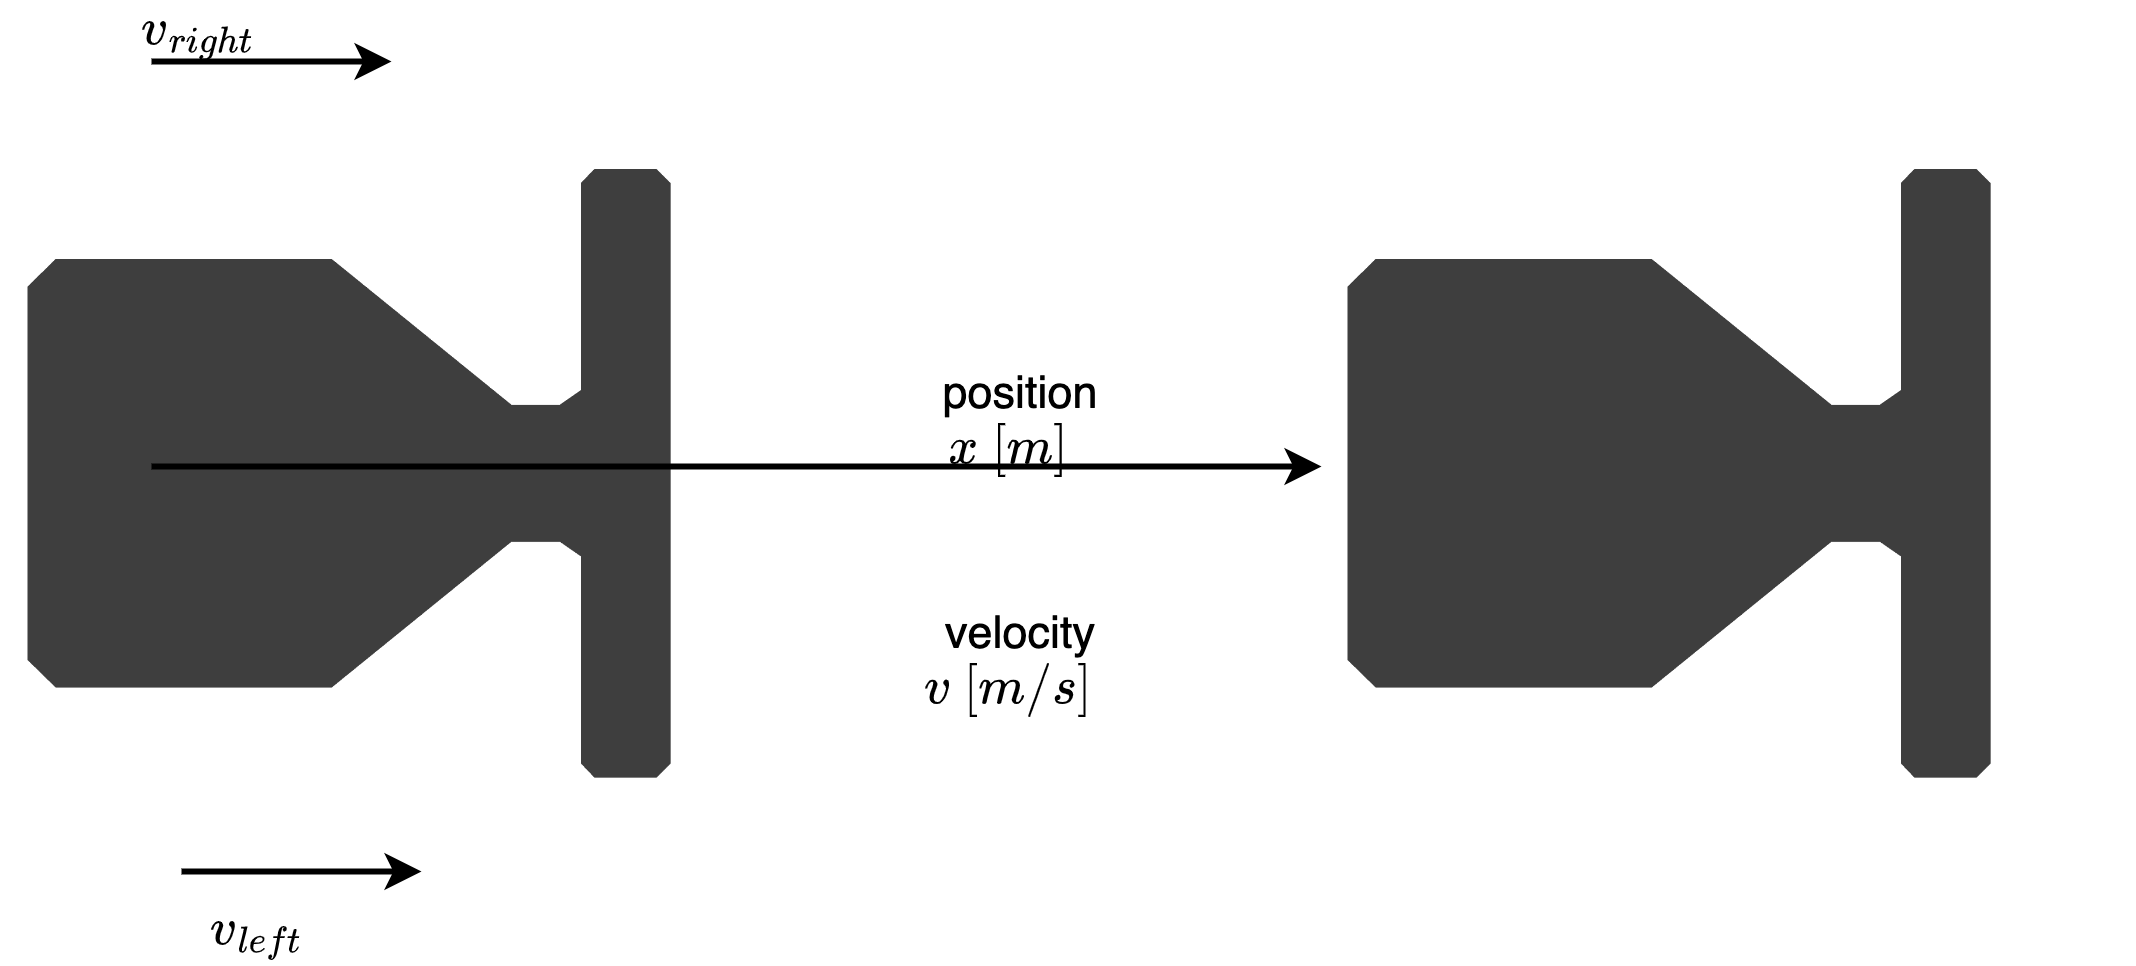
\includegraphics[scale=0.4]{../diagrams/robot_control/control-translation.png}}

\end{frame}

\begin{frame}
  
  \frametitle{\bf robot controll - rotation}

  \centering{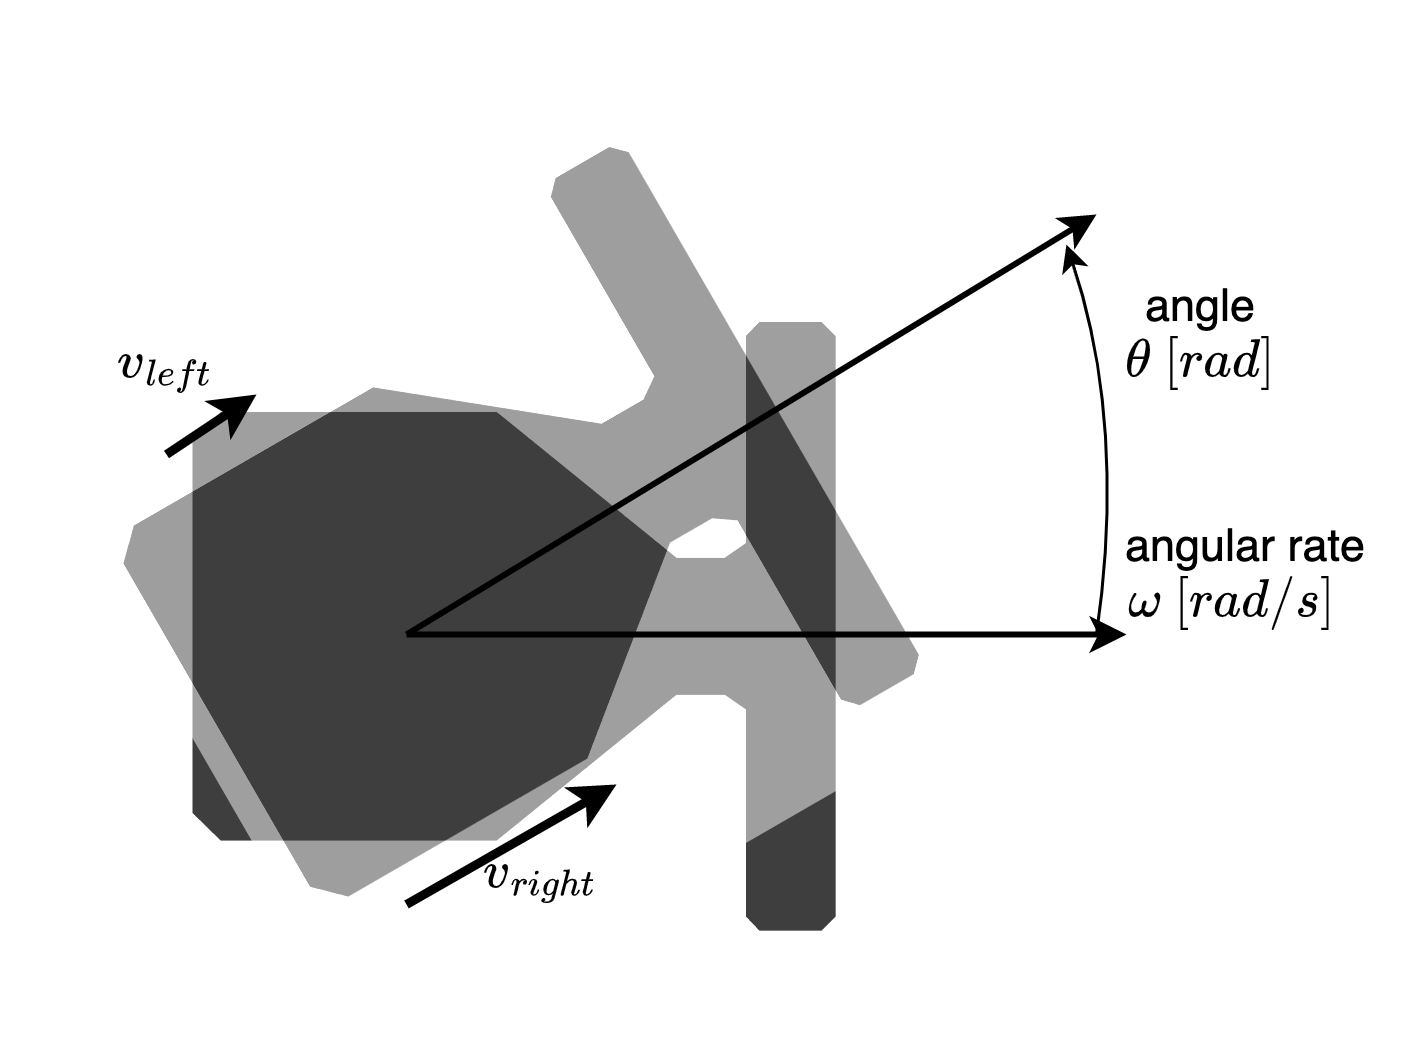
\includegraphics[scale=0.4]{../diagrams/robot_control/control-rotation.png}}

\end{frame}


\begin{frame}
  \frametitle{\bf robot controll - overview}

  \begin{itemize}
    \item position control : distance $x$ and angle $\theta$
    \item required values : $x_r$, $\theta_r$
    \item observed values : $x$, $\theta$ 
    \item forward  : $x_r(n) = x(n) + speed_{r}$
    \item turning  : $\theta_r(n) = \theta(n) + angular\_vel_{r}$
    \item full state vector : $(x, \theta, v, \omega)$
    \item note 1, : vectors are matrices, with shape $N x 1$
    \item note 2, : nice to have model of dynamics, \bf{planning}
  \end{itemize}

\end{frame}



\begin{frame}
  \frametitle{\bf controller loops}

  \centering{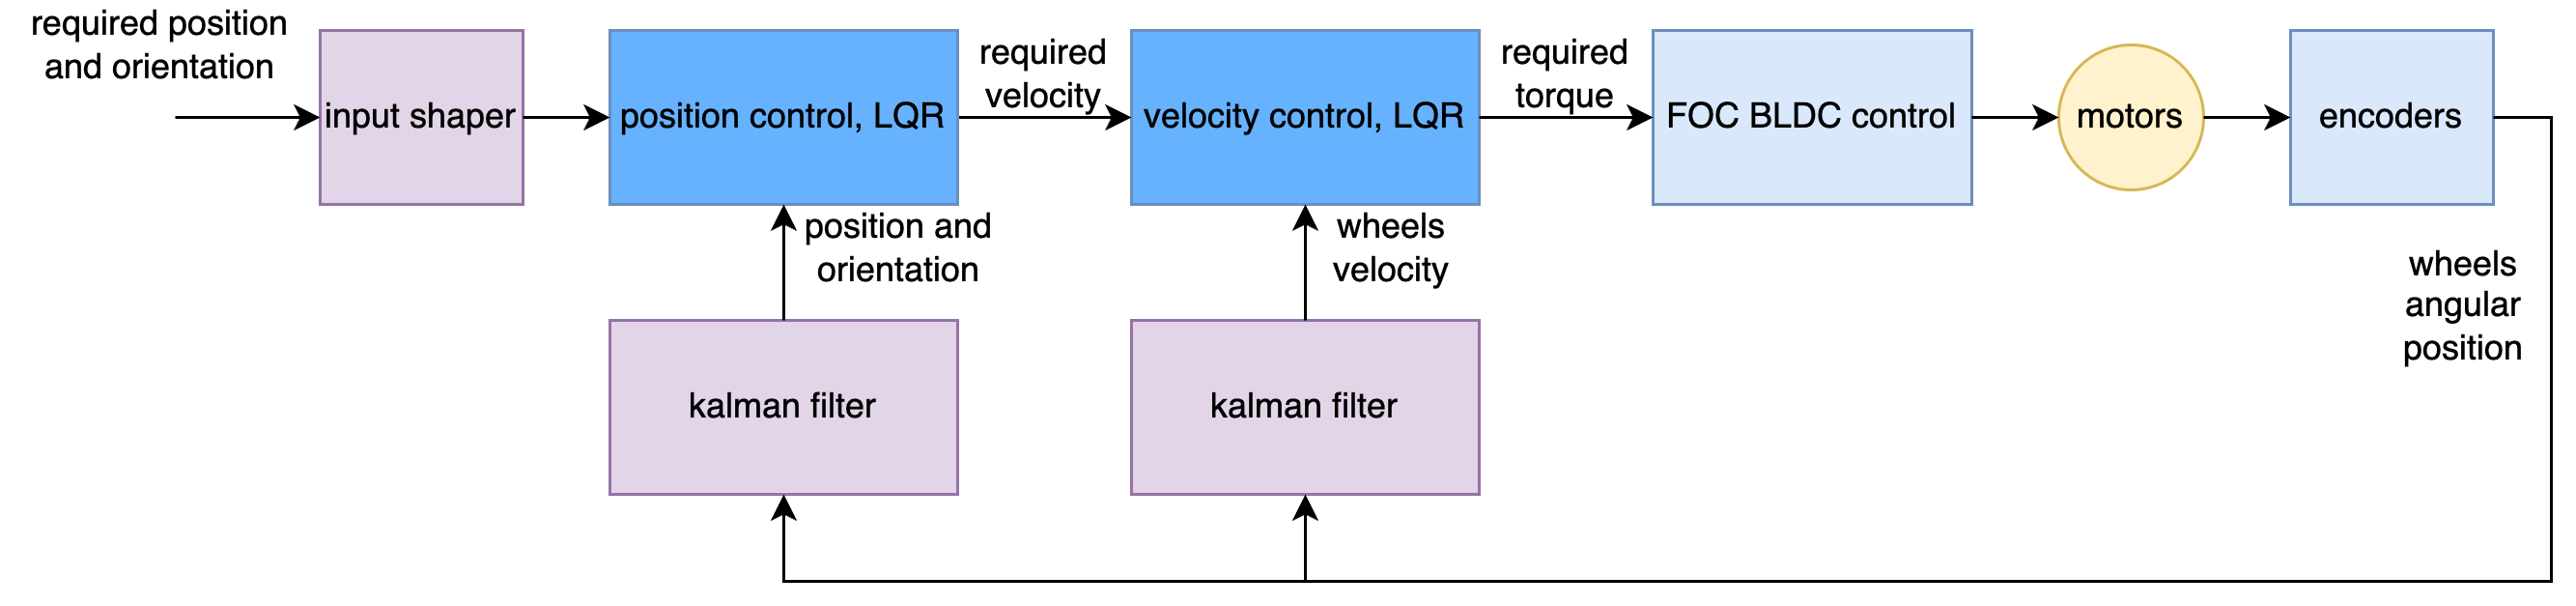
\includegraphics[scale=0.4]{../diagrams/robot_control/control-overview.png}}

  \begin{itemize}
    \item if we dont know system dynamics (only guessing) : 
      \begin{itemize}
        \item {\bf{if else}} controller
        \item hand tunned {\bf{PID}} controller
      \end{itemize}
    \item from known dynamics :
      \begin{itemize}
        \item Kalman filter
        \item LQR, LQG, H$\infty$
        \item {\bf{MPC}} - planning
      \end{itemize}
  \end{itemize}

\end{frame}




\begin{frame}
  
  \frametitle{\bf toy example - servo controll}

  \raggedright{{\bf open} loop response :}\\
  \centering{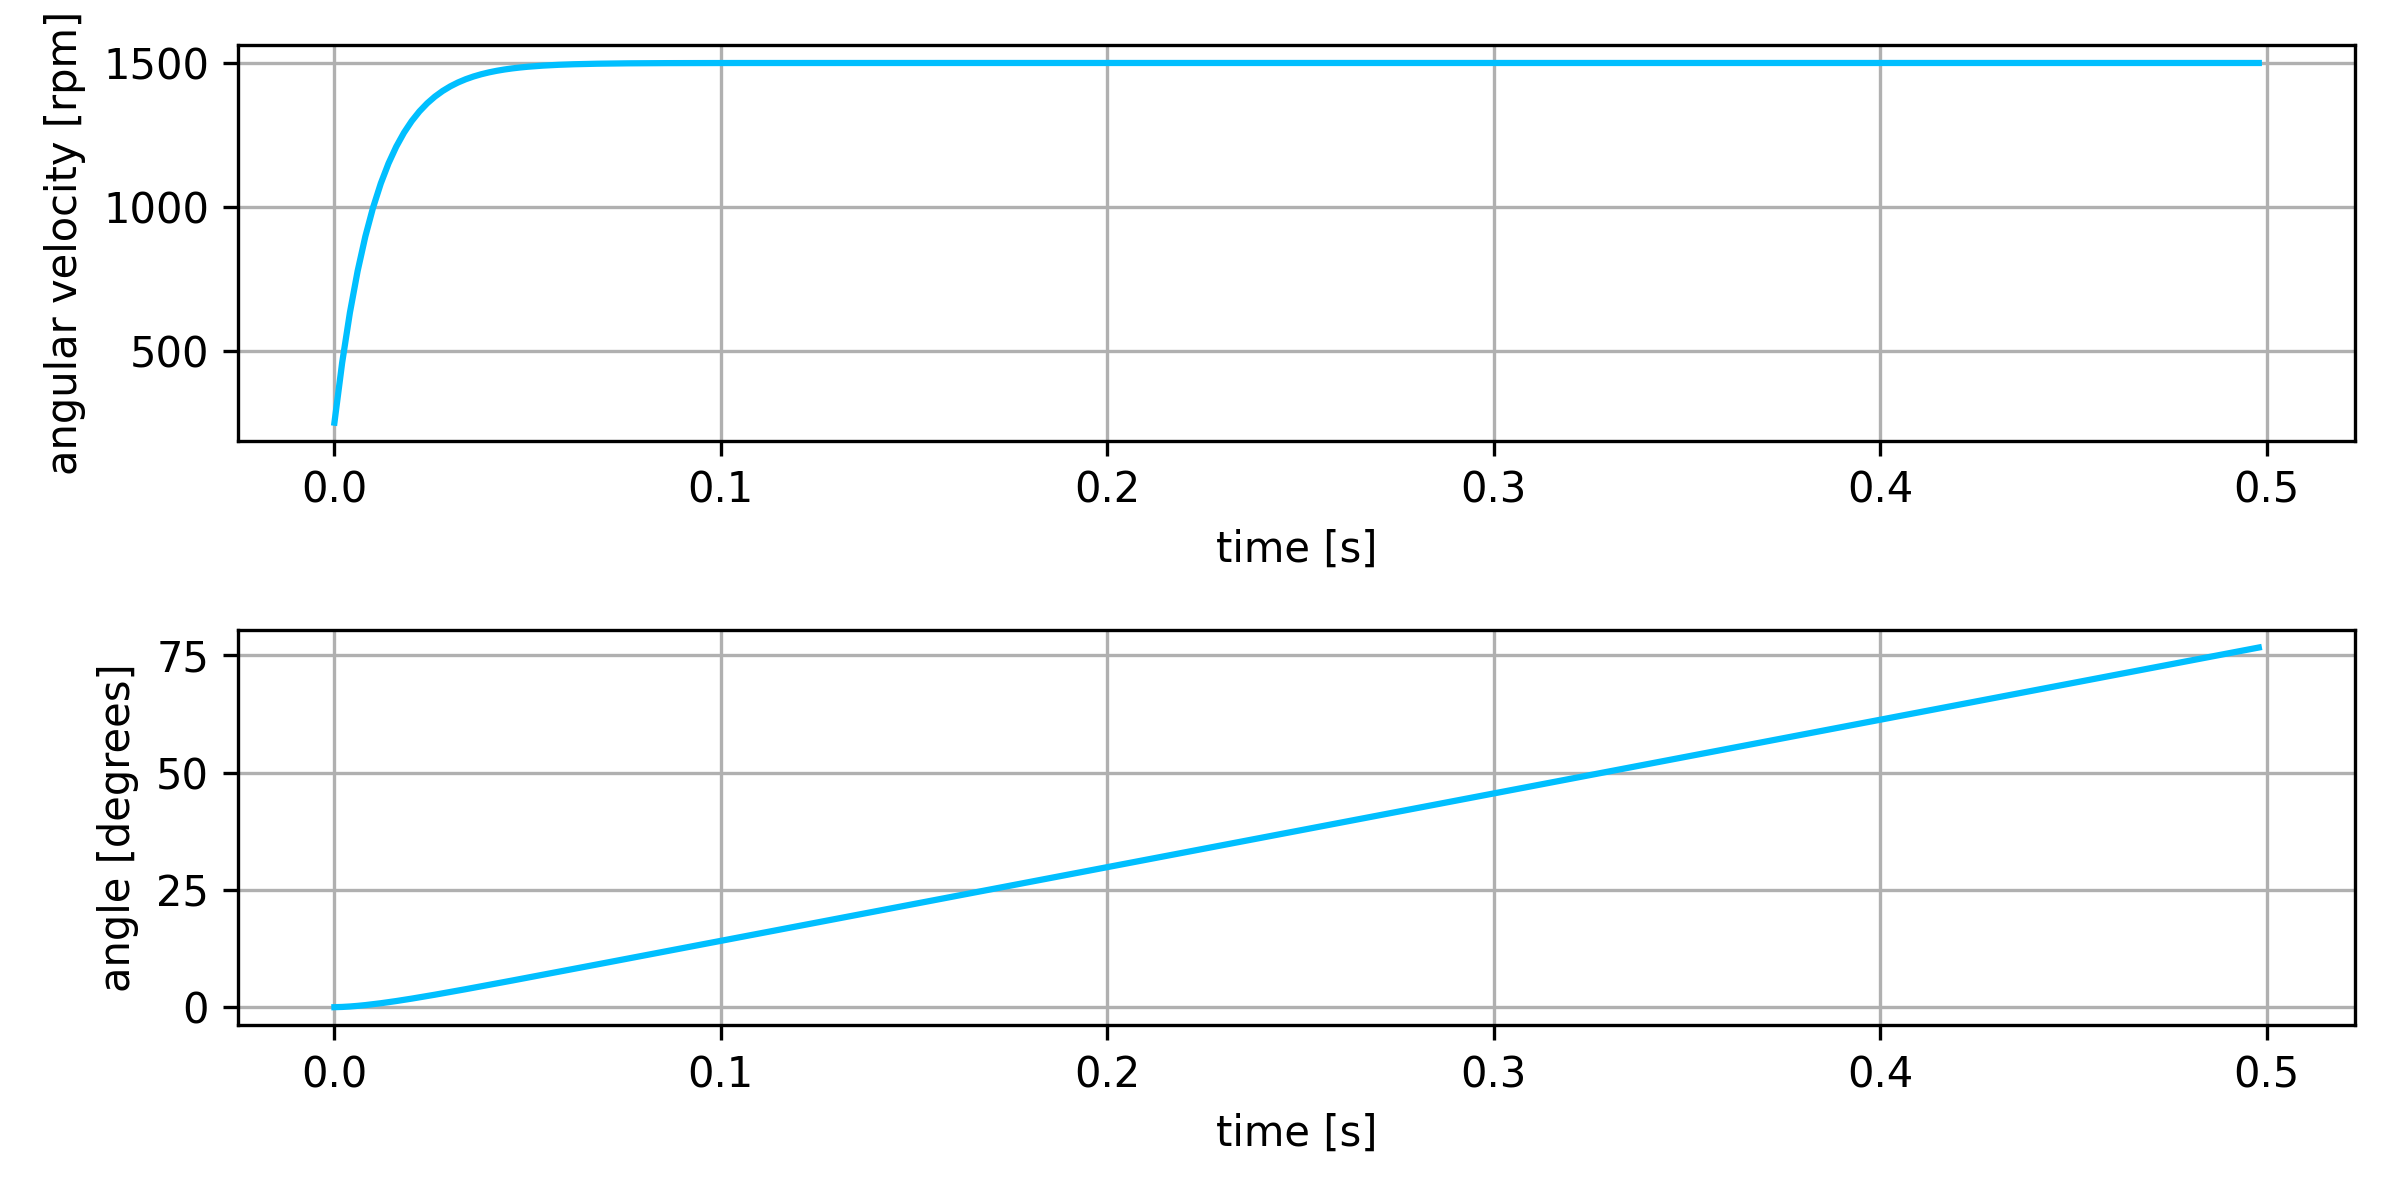
\includegraphics[scale=0.25]{../images/motors/open_loop_response.png}}
  
  \raggedright{{\bf closed} loop response (LQR controller) :}\\
  \centering{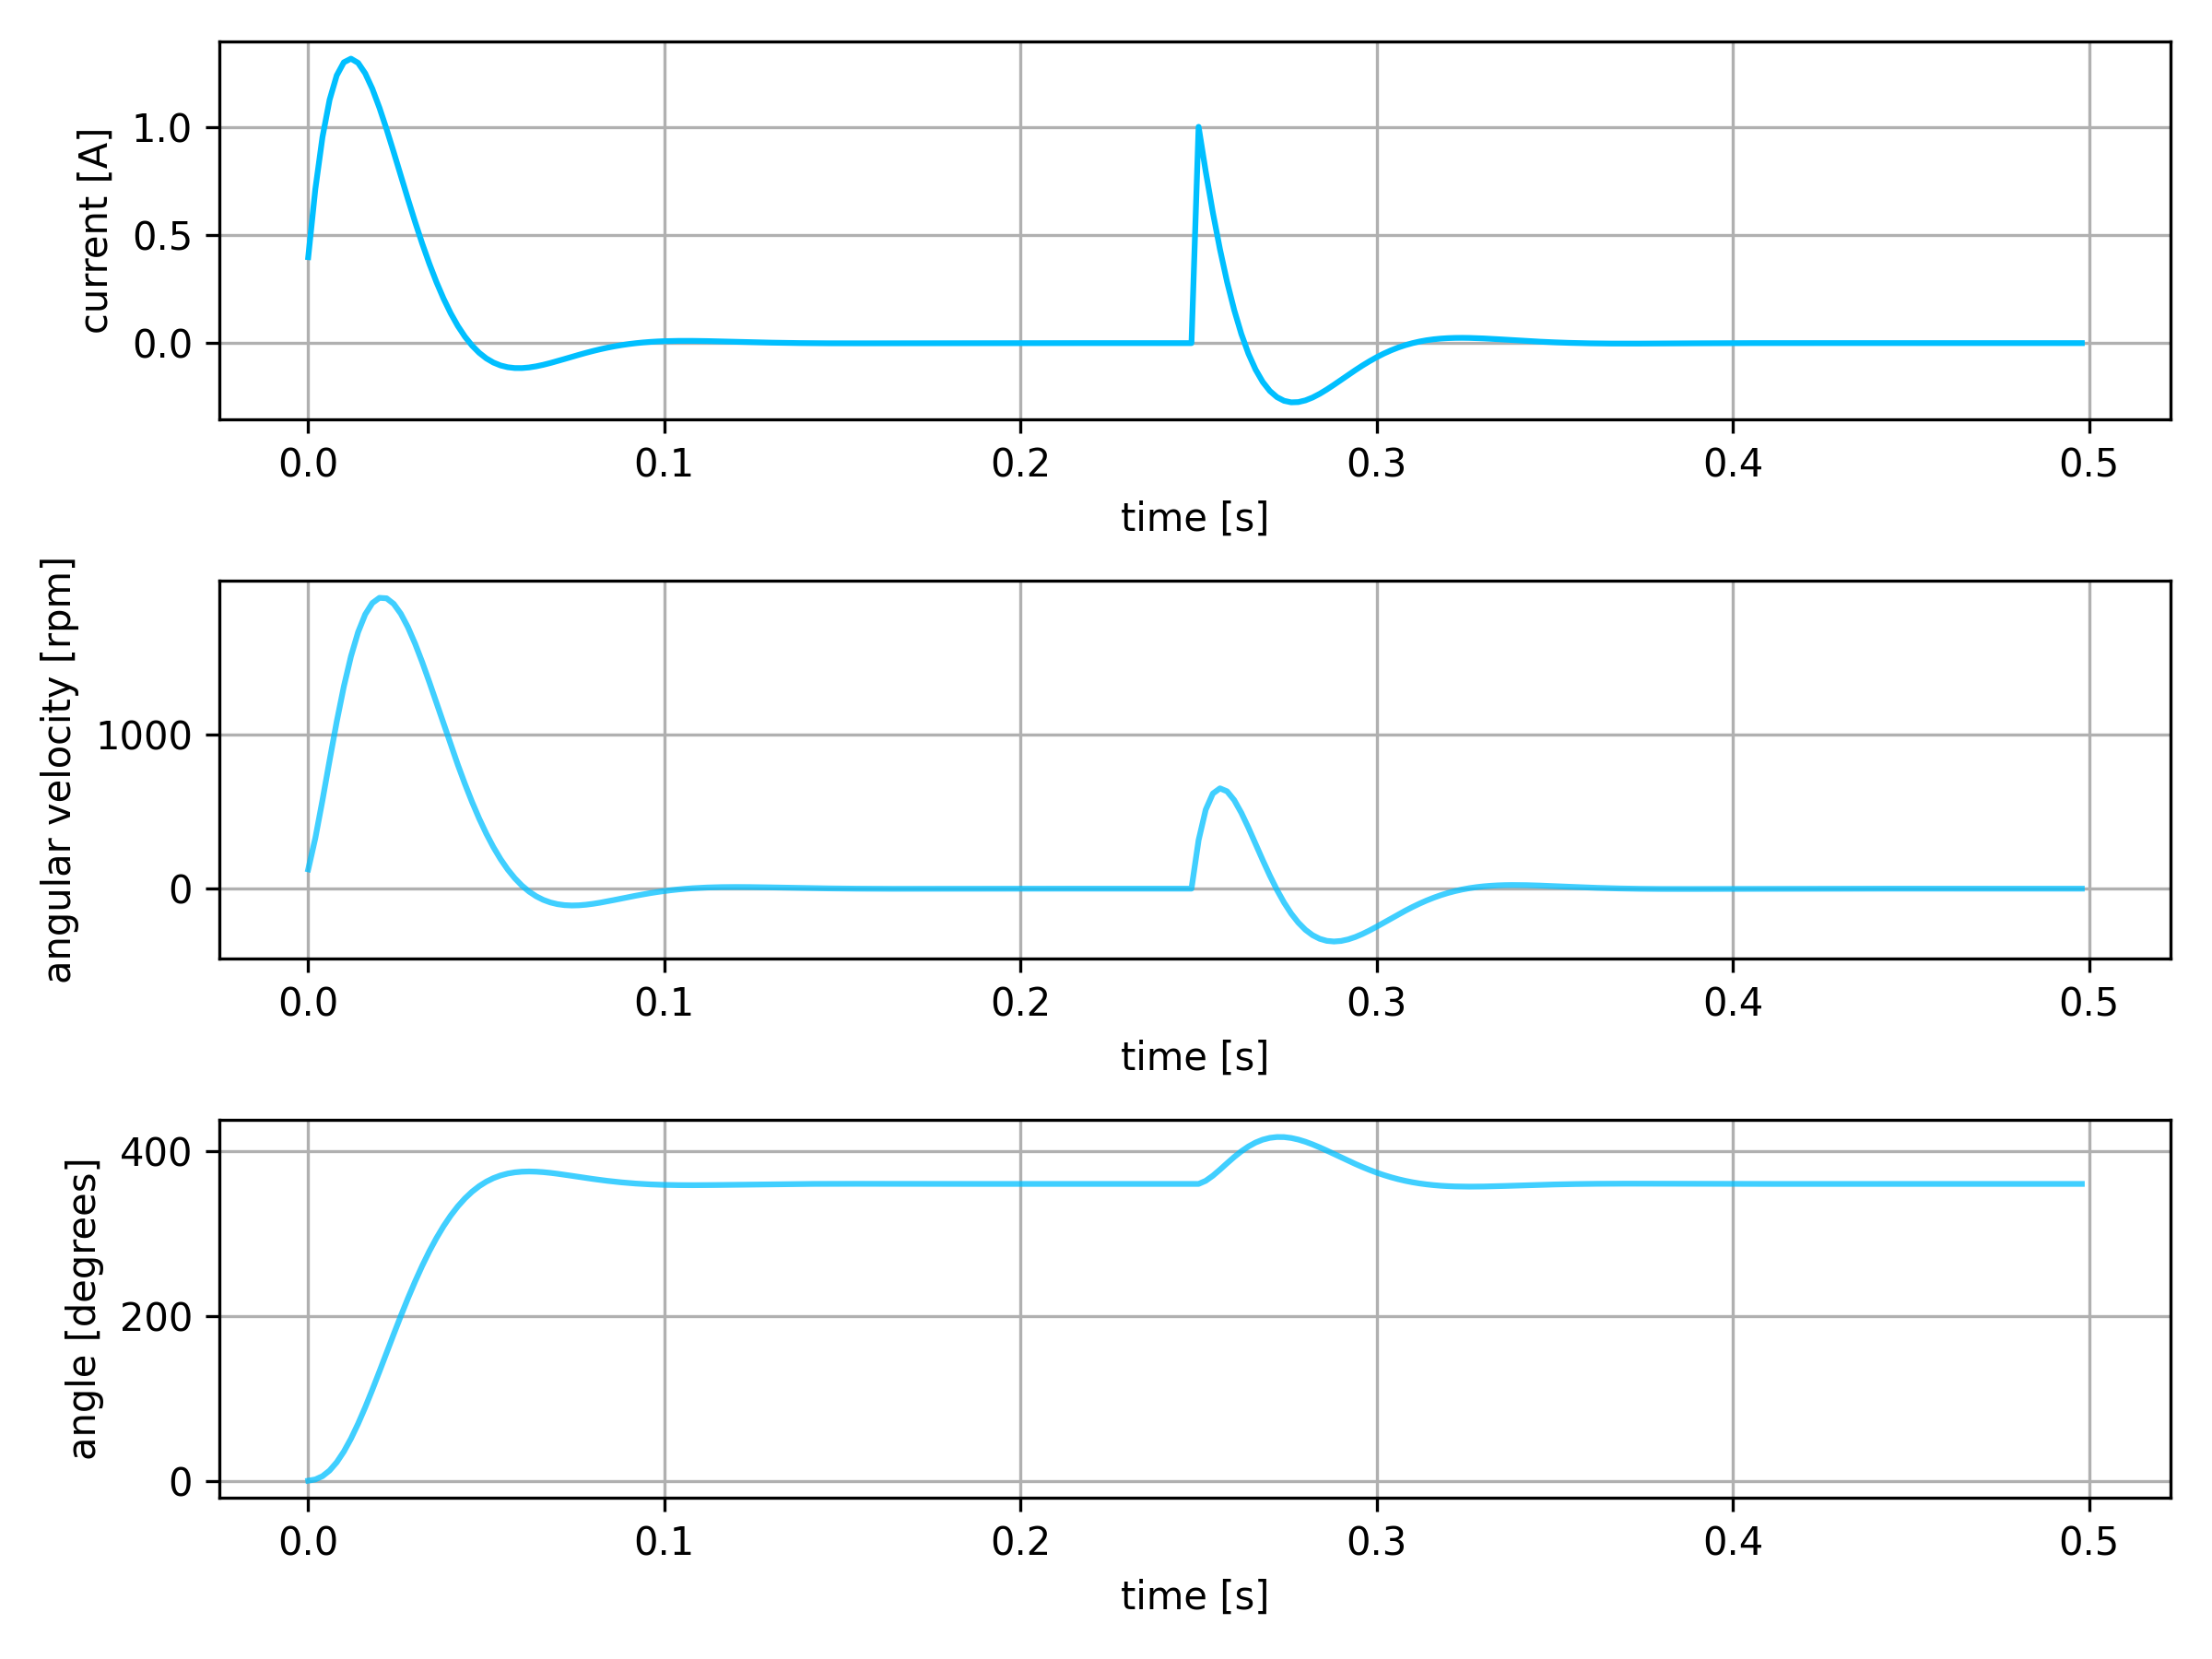
\includegraphics[scale=0.25]{../images/motors/closed_loop_response.png}}

\end{frame}


\begin{frame}
  
  \frametitle{\bf servo state space model}

  \centering{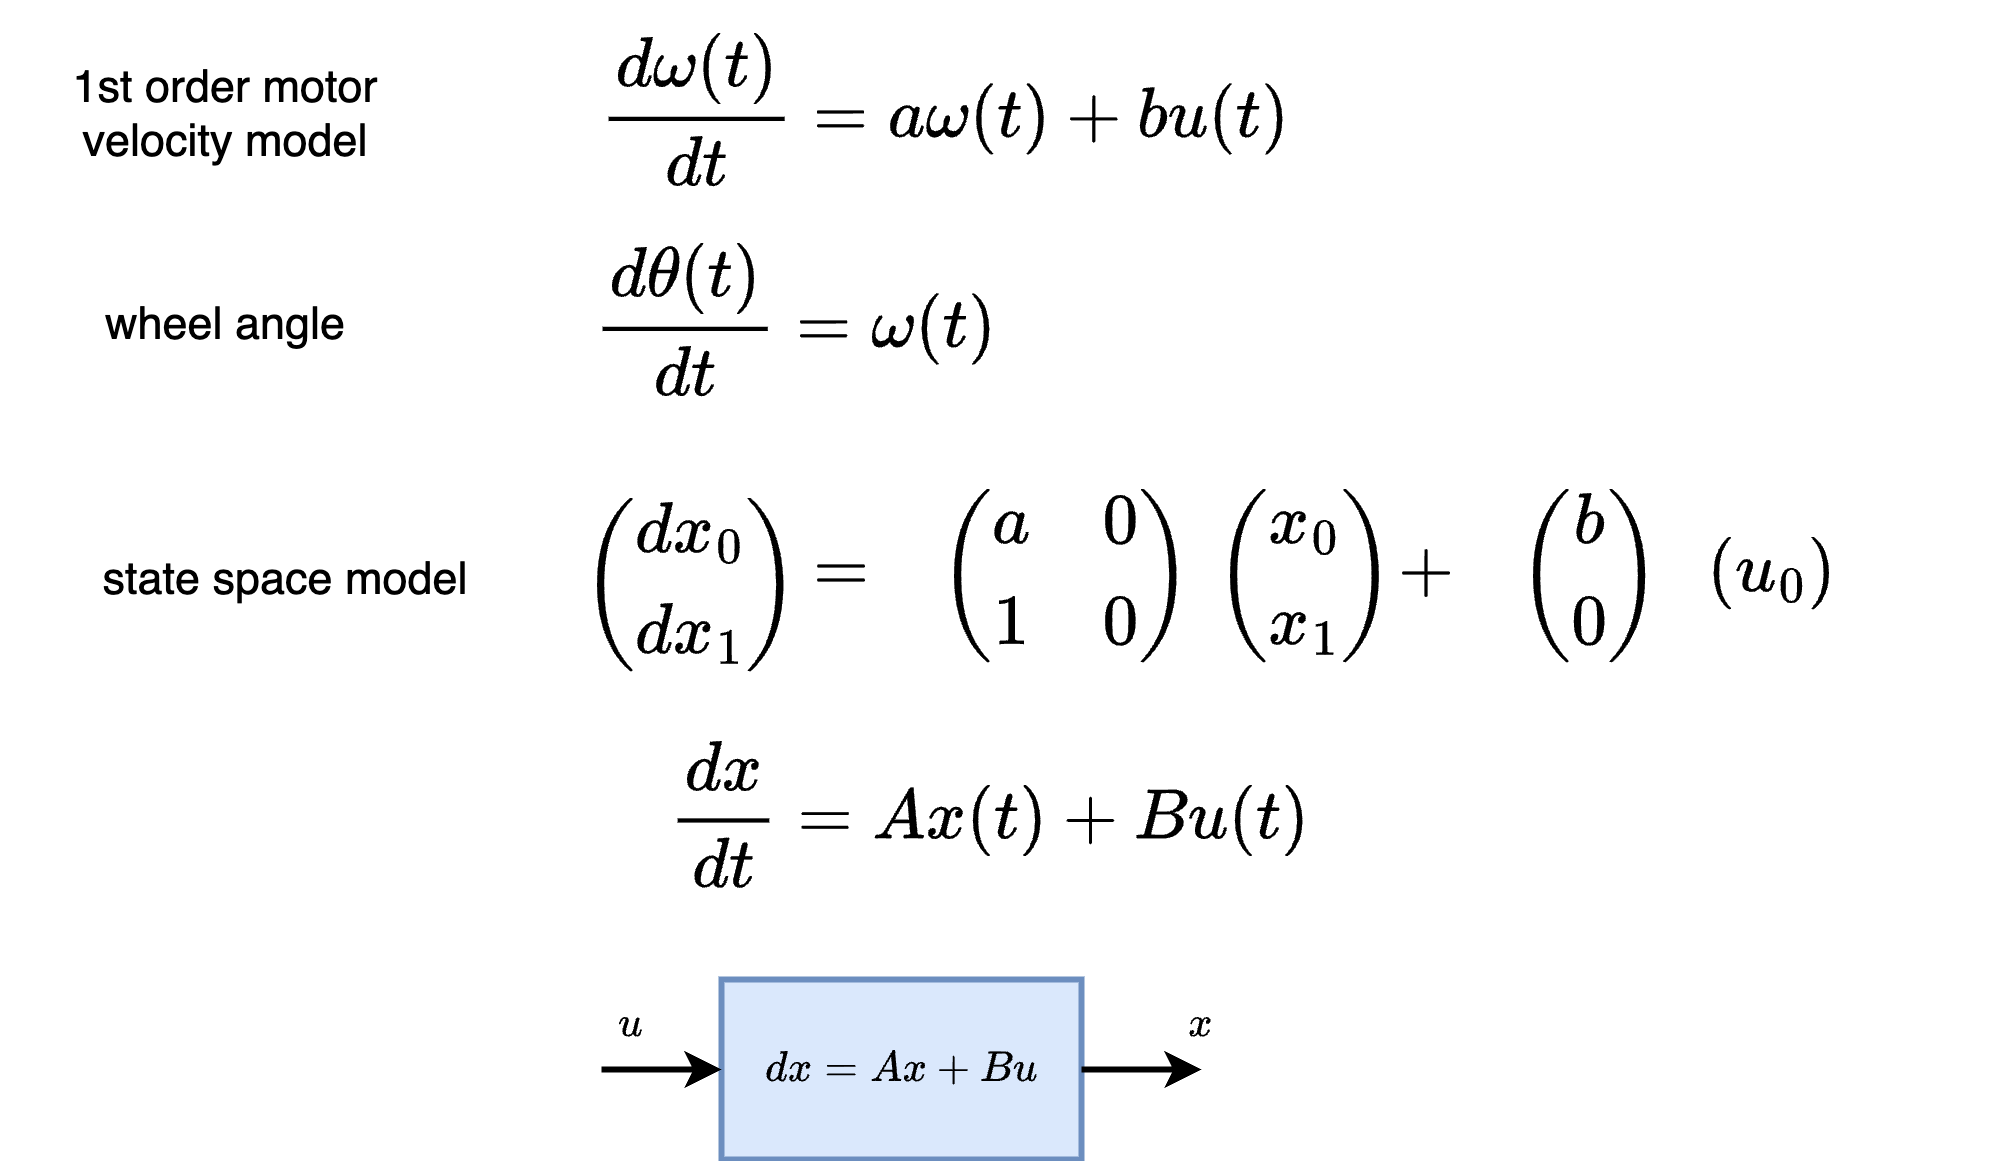
\includegraphics[scale=0.5]{../diagrams/robot_control/control-servo.png}}
  
\end{frame}




\begin{frame}
  \frametitle{\bf feedback loop}

  \centering{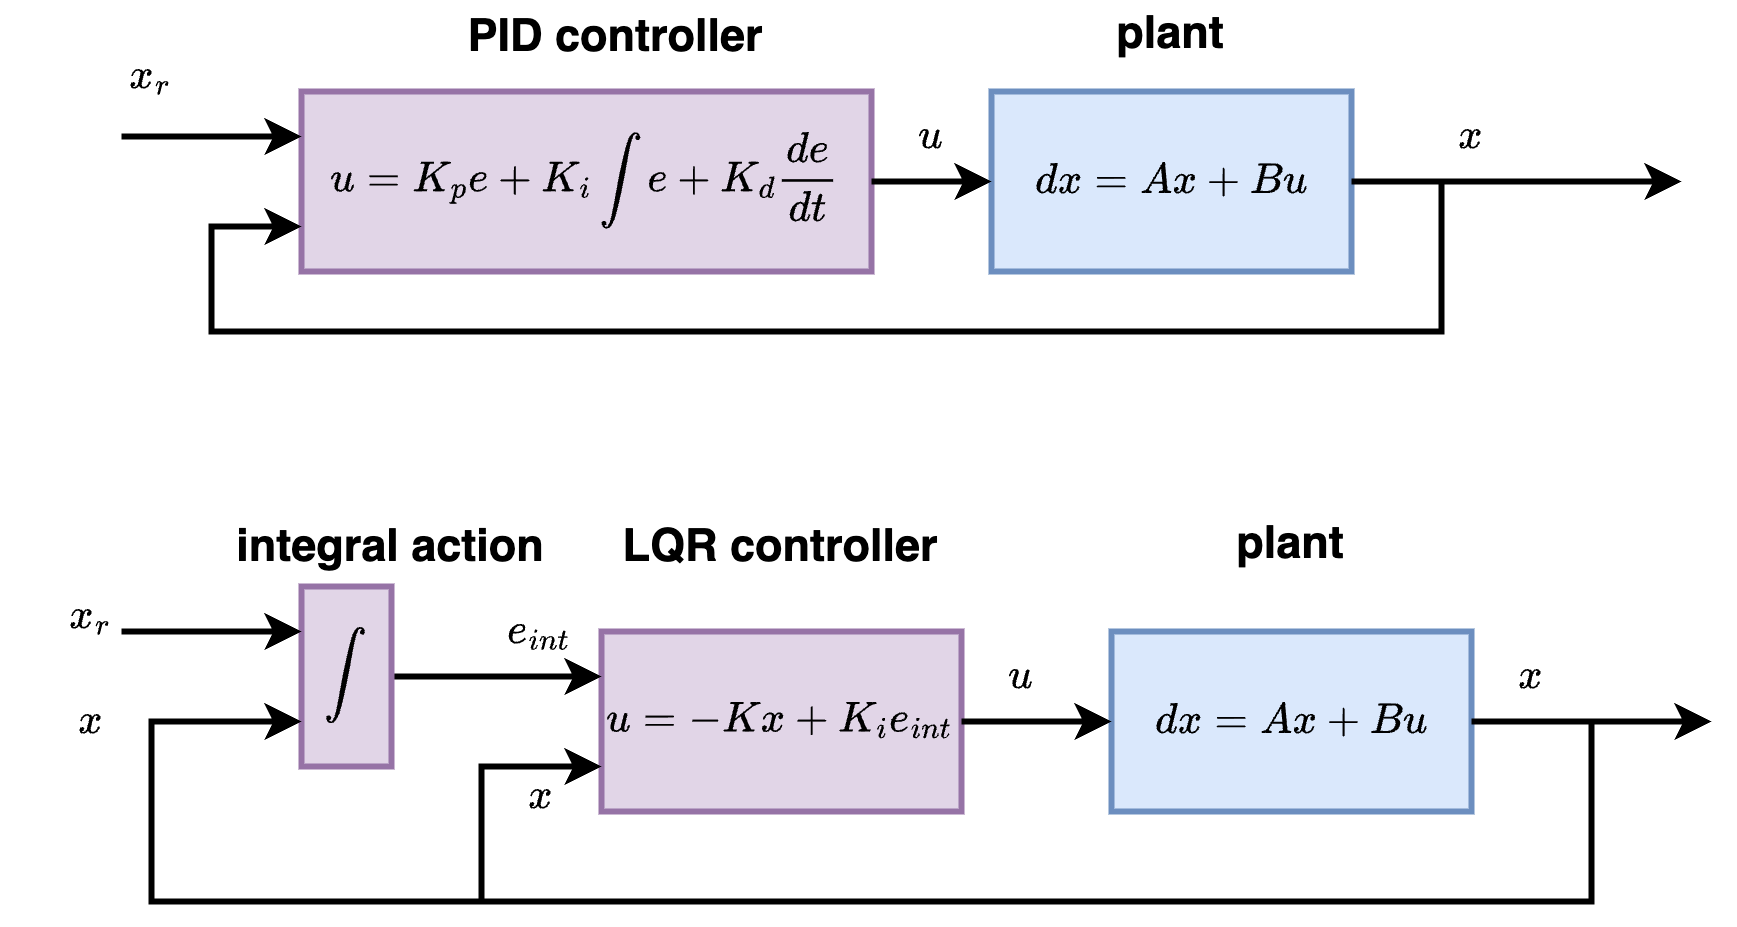
\includegraphics[scale=0.5]{../diagrams/robot_control/control-lqr_pid.png}}

  \begin{itemize}
    \item {\bf PID} : three {\bf \color{red} guessed} parameters, $K_p, K_i, K_d$
    \item {\bf LQR} : two {\bf \color{red} computed} matrices, $K, K_i$
  \end{itemize}

  note : continuos modeling (and controllers) have slow inference time - requires Runge-Kutta solvers,
  always use discrete models and controllers
\end{frame}



\begin{frame}
  \frametitle{\bf complete feedback loop}

  \centering{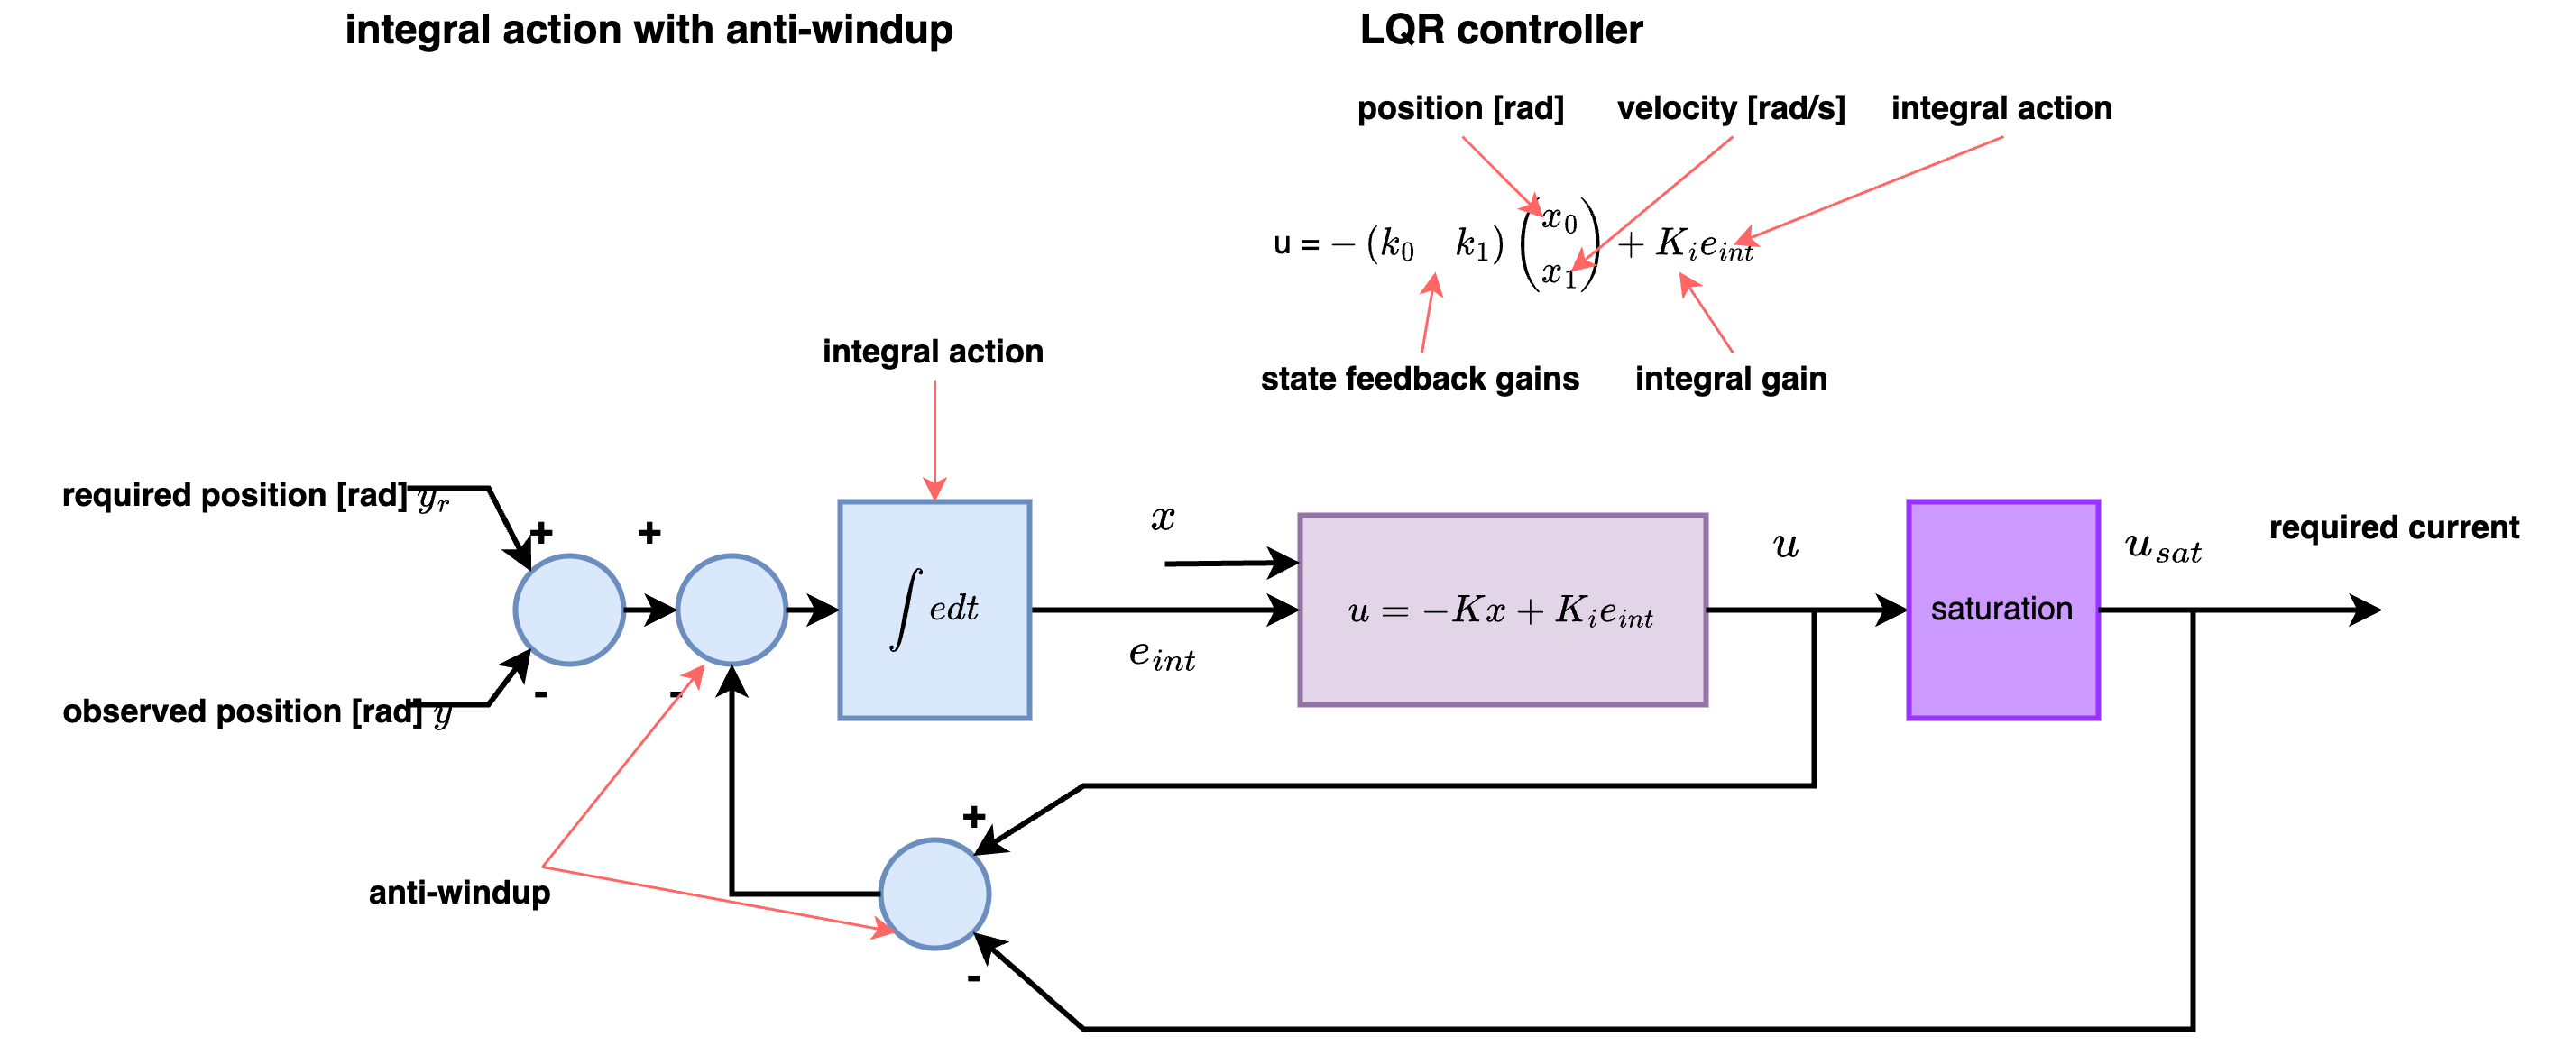
\includegraphics[scale=0.5]{../diagrams/robot_control/servo_control-lqr.png}}

  \begin{itemize}
    \item input : position $x_0$, velocity $x_1$, required position $x_r$
    \item output : current $u$
    \item integral action : $e_{int}(t) = \int_0^t x_r - x_0 d\tau $
    \item LQR : $u = -Kx + K_ie_{int}$
  \end{itemize}
\end{frame}


\begin{frame}
  \frametitle{\bf discrete linear state space model}

  \centering{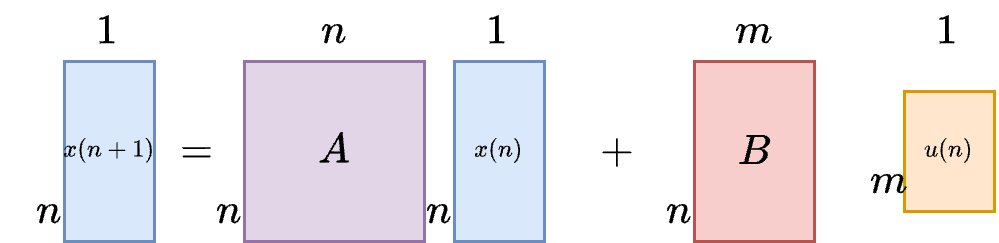
\includegraphics[scale=1.0]{../diagrams/identification/identification-system_dynamics.png}}

  \begin{align*}
    x(n+1) &= Ax(n) + Bu(n)
  \end{align*}

  \begin{itemize}
    \item $n$ : system order, $m$ : system inputs count
    \item $x(n)$ - system state, matrix $n \times 1$
    \item $u(n)$ - control input, matrix $m \times 1$
    \item $A$    - transient matrix, $n \times n$
    \item $B$    - input matrix, $n \times m$
  \end{itemize}

\end{frame}

\begin{frame}
  \frametitle{\bf toy example - kalman filter object tracking}
  \centering{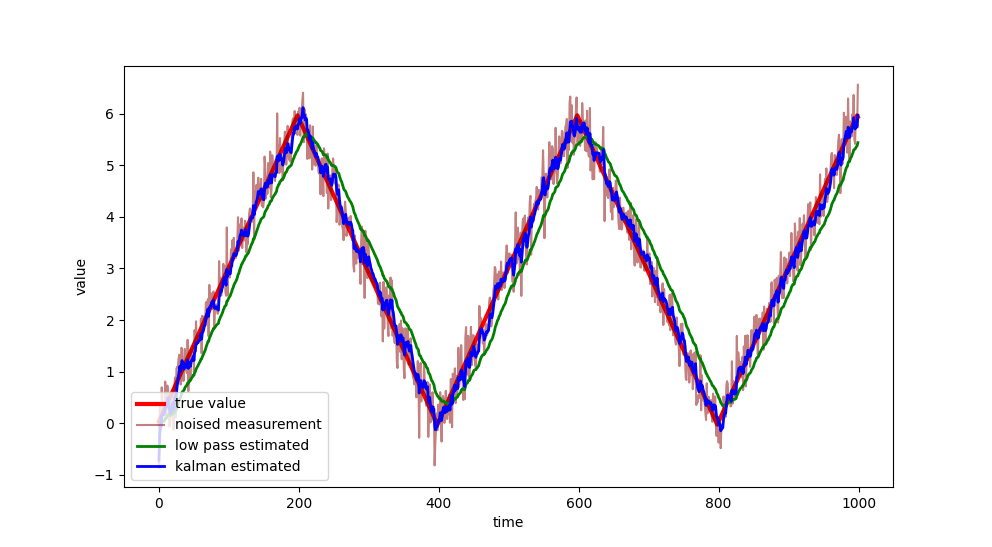
\includegraphics[scale=0.3]{../images/kalman_tracking.png}}

  low pass filter (exponential moving average)
  \begin{align*}
    \hat{x}(n+1) = \alpha \hat{x}(n) + (1 - \alpha)x(n)
  \end{align*}

  kalman filter
  \begin{align*}
    \hat{x}(n+1) & = A \hat{x}(n) + K( x(n) - \hat{x}(n)) \\
    \hat{x}(n+1) & = A \hat{x}(n) + Bu(n) + K( x(n) - \hat{x}(n))
  \end{align*}

\end{frame}




\begin{frame}
  \frametitle{\bf toy example - kalman filter object tracking}

  constant position model 
  
  \begin{align*}
    \begin{pmatrix}
      x
    \end{pmatrix}_{n+1} = 
    \begin{pmatrix}
      1
    \end{pmatrix}
    \begin{pmatrix}
      x
    \end{pmatrix}_{n}
  \end{align*}
  
  constant velocity model 
  
  \begin{align*}
    \begin{pmatrix}
      v \\
      x
    \end{pmatrix}_{n+1} = 
    \begin{pmatrix}
      1 & 0 \\
      1 & 1
    \end{pmatrix}
    \begin{pmatrix}
      v \\
      x
    \end{pmatrix}_{n}
  \end{align*}


  constant acceleration model 
  
  \begin{align*}
    \begin{pmatrix}
      a \\
      v \\
      x \\
    \end{pmatrix}_{n+1} = 
    \begin{pmatrix}
      1 & 0 & 0 \\
      1 & 1 & 0 \\
      0 & 1 & 1
    \end{pmatrix}
    \begin{pmatrix}
      a \\
      v \\
      x \\
    \end{pmatrix}_{n}
  \end{align*}


\end{frame}




\begin{frame}
  \frametitle{\bf red pill section}
\end{frame}



\begin{frame}
  \frametitle{\bf LQR - optimal control}

  controller
  \begin{align*}
    u(n) = -Kx(n)
  \end{align*}
  
  loss (cost) function is quadratic, with weighting terms $Q$ and $R$
  \begin{align*}
    \mathcal{L} &=\sum_n^{\infty} x^T(n) Q x(n) + u^T(n) R u(n) \\
    s.t. \quad x(n+1) &= Ax(n) + Bu(n) 
  \end{align*}  

  matrix K is obtained by solving Riccati ARE
  \begin{align*}
    P(n-1) &= Q + A^TP(n)A - A^TP(n)B(B^TP(n) + R)^{-1}B^TP(n)A \\
    where \quad P(\infty) &= Q \\
    K &= R^{-1}B^TP(0)
  \end{align*}

\end{frame}

\begin{frame}
  
  \frametitle{\bf system identification}

  \begin{itemize}
    \item generate input sequence : $u$
    \item measure data : $x$
    \item fitting model $\hat{A}$, $\hat{B}$ into data
    \item predicted data : $\hat{x}$
  \end{itemize}
  
  \begin{align*}
    \mathcal{L} &= \sum_{n=0}^{N} (x(n) - \hat{x}(n))^2 \\
    s.t. \quad \hat{x}(n+1) &= \hat{A}x(n) + \hat{B}u(n)
  \end{align*}
 
  
\end{frame}


\begin{frame}
  
  \frametitle{\bf system identification}
  we can stack  $x$ and $u$ into single matrix $\tilde{X}$ 
  
  \centering{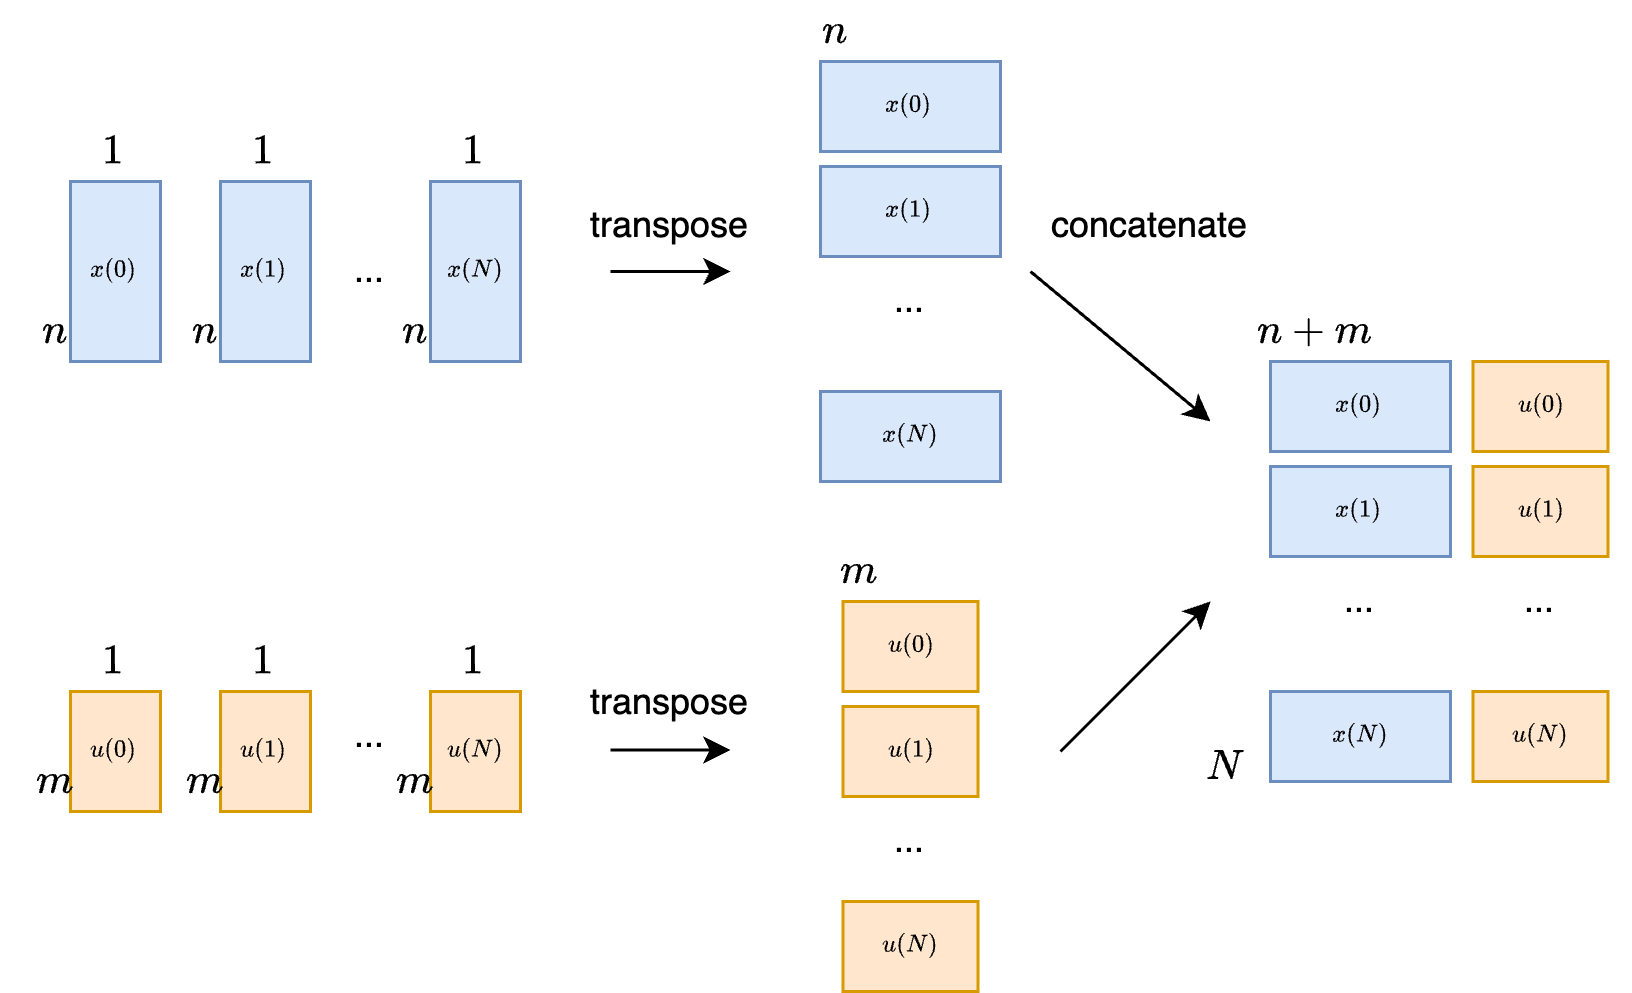
\includegraphics[scale=0.5]{../diagrams/identification/identification-arange}}

  same for matrices $\hat{A}$, $\hat{B}$  into $\tilde{M}$, \\
  also for $\hat{x}$ : $\hat{X}$, to get compact form 

  \begin{align*}
    \hat{X} &= \tilde{M}\tilde{X}
  \end{align*}

\end{frame}

\begin{frame}
  
  \frametitle{\bf system identification - least squares}

  \begin{align*}
    \hat{X} &= \tilde{M}\tilde{X}
  \end{align*}
  
  {\bf which is the least squares problems} \\
  can be solved by Moore-Penrose matrix pseudoinverse
  $\tilde{M} = numpy.linalg.lstsq(\tilde{X}, X)$

\end{frame}




\begin{frame}
  
  \frametitle{\bf model predictive control}

  loss (cost) function is quadratic, with weighting terms $Q$ and $R$,

  \begin{align*}
    \mathcal{L} &=\sum_h^{H-1} x^T(h) Q x(h) + du^T(h) R _\Delta u(h) \\
    u(n) & = u(n-1) + _\Delta u(n) \\
    s.t. \quad x(n+1) &= Ax(n) + Bu(n) 
  \end{align*}  

  where : 
  \begin{itemize}
    \item $H$ is prediction horizon steps
    \item $A$ is matrix, $n \times n$
    \item $B$ is matrix, $n \times m$
    \item $Q$ is matrix, $n \times n$
    \item $R$ is matrix, $m \times m$
    \item $_\Delta u$ is controller output
    \item where $n$ is system orders, and $m$ system inputs count
  \end{itemize}

  
\end{frame}


\begin{frame}
  
  \frametitle{\bf model predictive control}
  unwrap into form where only $x(n)$ is used to predict all other $x$
  \begin{align*}
    x(n+1)&= Ax(n) + Bu(n) \\
          &= Ax(n) + B(u(n-1) + _\Delta u(n)) \\
    x(n+2)&= Ax(n+1) + B(u(n) + _\Delta u(n+1)) \\
          &= A^2x(n) + (AB + B)u(n-1) + (AB+B)_\Delta u(n) + B_\Delta u(u) \\
    x(n+3)&= Ax(n+2) + B(u(n+1) + _\Delta u(n+2)) \\
          &= A^3x(n) + (A^2 + AB + B)u(n-1) 
          & + (A^2B + AB + B)_\Delta u(n) \\
          & + (AB + B)_\Delta u(n+1) + B_\Delta u(n+2) \\
    ... 
  \end{align*}  

  
\end{frame}






\begin{frame}
  
  \frametitle{\bf model predictive control}
  rewrite into matrix form
  \begin{align*}
    \begin{bmatrix}
      x(n+1) \\
      x(n+2) \\
      \dots \\
      x(n+H)
    \end{bmatrix} &= 
    \begin{bmatrix}
      A^1 \\
      A^2 \\
      \dots \\
      A^H
    \end{bmatrix} x(n) +
    \begin{bmatrix}
      B \\
      AB \\
      \dots \\
      \sum_{i=0}^{H-1} A^iB
    \end{bmatrix} u(n-1) + \\
    &+
    \begin{bmatrix}
      B  & 0 & \dots & 0 \\
      AB + B & B & \dots & 0 \\
      \dots & \dots & \dots & \dots \\
      \sum_{i=0}^{H-1}A^iB & \sum_{i=0}^{H-2}A^iB & \dots & B
    \end{bmatrix}
    \begin{bmatrix}
      _\Delta u(n) \\
      \dots \\
      _\Delta u(n + H - 1) \\
    \end{bmatrix} 
  \end{align*}

  in compat form

  \begin{align*}
    \tilde{X} &= \Psi x(n) + \Omega u(n-1) + \Theta \tilde{_\Delta U}
  \end{align*}


\end{frame}








\begin{frame}
  
  \frametitle{\bf model predictive control}

  quadratic loss (cost) function

  \begin{align*}
    \mathcal{L} &= \tilde{_\Delta U}^T \tilde{R} \tilde{_\Delta U} 
                + (\tilde{X_r} - \tilde{X})^T \tilde{Q} (\tilde{X_r} - \tilde{X})^T \\
  \end{align*}

  after substitution
  \begin{align*}
    S = \tilde{X_r} - \Psi\tilde{X} - \Omega u(n-1)
  \end{align*}


  \begin{align*}
    \mathcal{L} &= \tilde{_\Delta U}^T \tilde{R} \tilde{_\Delta U} + (S -  \Theta \tilde{_\Delta U} )^T \tilde{Q} (S -  \Theta \tilde{_\Delta U} ) \\
                &= \tilde{_\Delta U}^T \tilde{R} \tilde{_\Delta U} 
                + S^T\tilde{Q}S - S^T \tilde{Q} \Theta \tilde{_\Delta U} 
                - \tilde{_\Delta U}^T \Theta^T\tilde{Q}S + \tilde{_\Delta U}^T\Theta^T\tilde{Q}\Theta\tilde{_\Delta U}
  \end{align*}

\end{frame}



\begin{frame}
  
  \frametitle{\bf model predictive control}

  find derivative with respect to $\tilde{_\Delta U}$ 

  \begin{align*}
    \frac{\partial \mathcal{L}}{\partial {\tilde{_\Delta U}}} & : \\
    \frac{\partial {\tilde{_\Delta U}^T \tilde{R} \tilde{_\Delta U} } }{\partial {\tilde{_\Delta U}}} & = 2\tilde{R}\tilde{_\Delta U} \\
    \frac{\partial {S^T\tilde{Q}S}}{\partial {\tilde{_\Delta U}}} & = 0 \\
    \frac{\partial {- S^T \tilde{Q} \Theta \tilde{_\Delta U} }}{\partial {\tilde{_\Delta U}}} & = -\Theta^T\tilde{Q}S \\
    \frac{\partial {- \tilde{_\Delta U}^T \Theta^T\tilde{Q}S}}{\partial {\tilde{_\Delta U}}} & = -\Theta^T\tilde{Q}S \\
    \frac{\partial { \tilde{_\Delta U}^T\Theta^T\tilde{Q}\Theta\tilde{_\Delta U}}}{\partial {\tilde{_\Delta U}}} & = 2\Theta^T\tilde{Q}\Theta\tilde{_\Delta U}
  \end{align*}  

\end{frame}


\begin{frame}
  
  \frametitle{\bf model predictive control}

  put derivate equal to zero, and solve

  \begin{align*}
    \frac{\partial \mathcal{L}}{\partial {\tilde{_\Delta U}}} & = 2 \tilde{R} \tilde{_\Delta U} - 2\Theta^T\tilde{Q}S + 2\Theta^T\tilde{Q}\Theta\tilde{_\Delta U} \\
    0 &= 2 \tilde{R} \tilde{_\Delta U} - 2\Theta^T\tilde{Q}S + 2\Theta^T\tilde{Q}\Theta\tilde{_\Delta U} \\
    (\tilde{R} + \Theta^T\tilde{Q}\Theta)\tilde{_\Delta U}  &= \Theta^T\tilde{Q}S 
  \end{align*}  

  and obtain solution for model predictive controll
  \begin{align*}
    \tilde{_\Delta U} &= (\tilde{R} + \Theta^T\tilde{Q}\Theta)^{-1} \Theta^T\tilde{Q}S
  \end{align*} 

\end{frame}


\begin{frame}
  
  \frametitle{Q\&A}

  \begin{columns}

    \begin{column}{0.5\textwidth}
      \centering{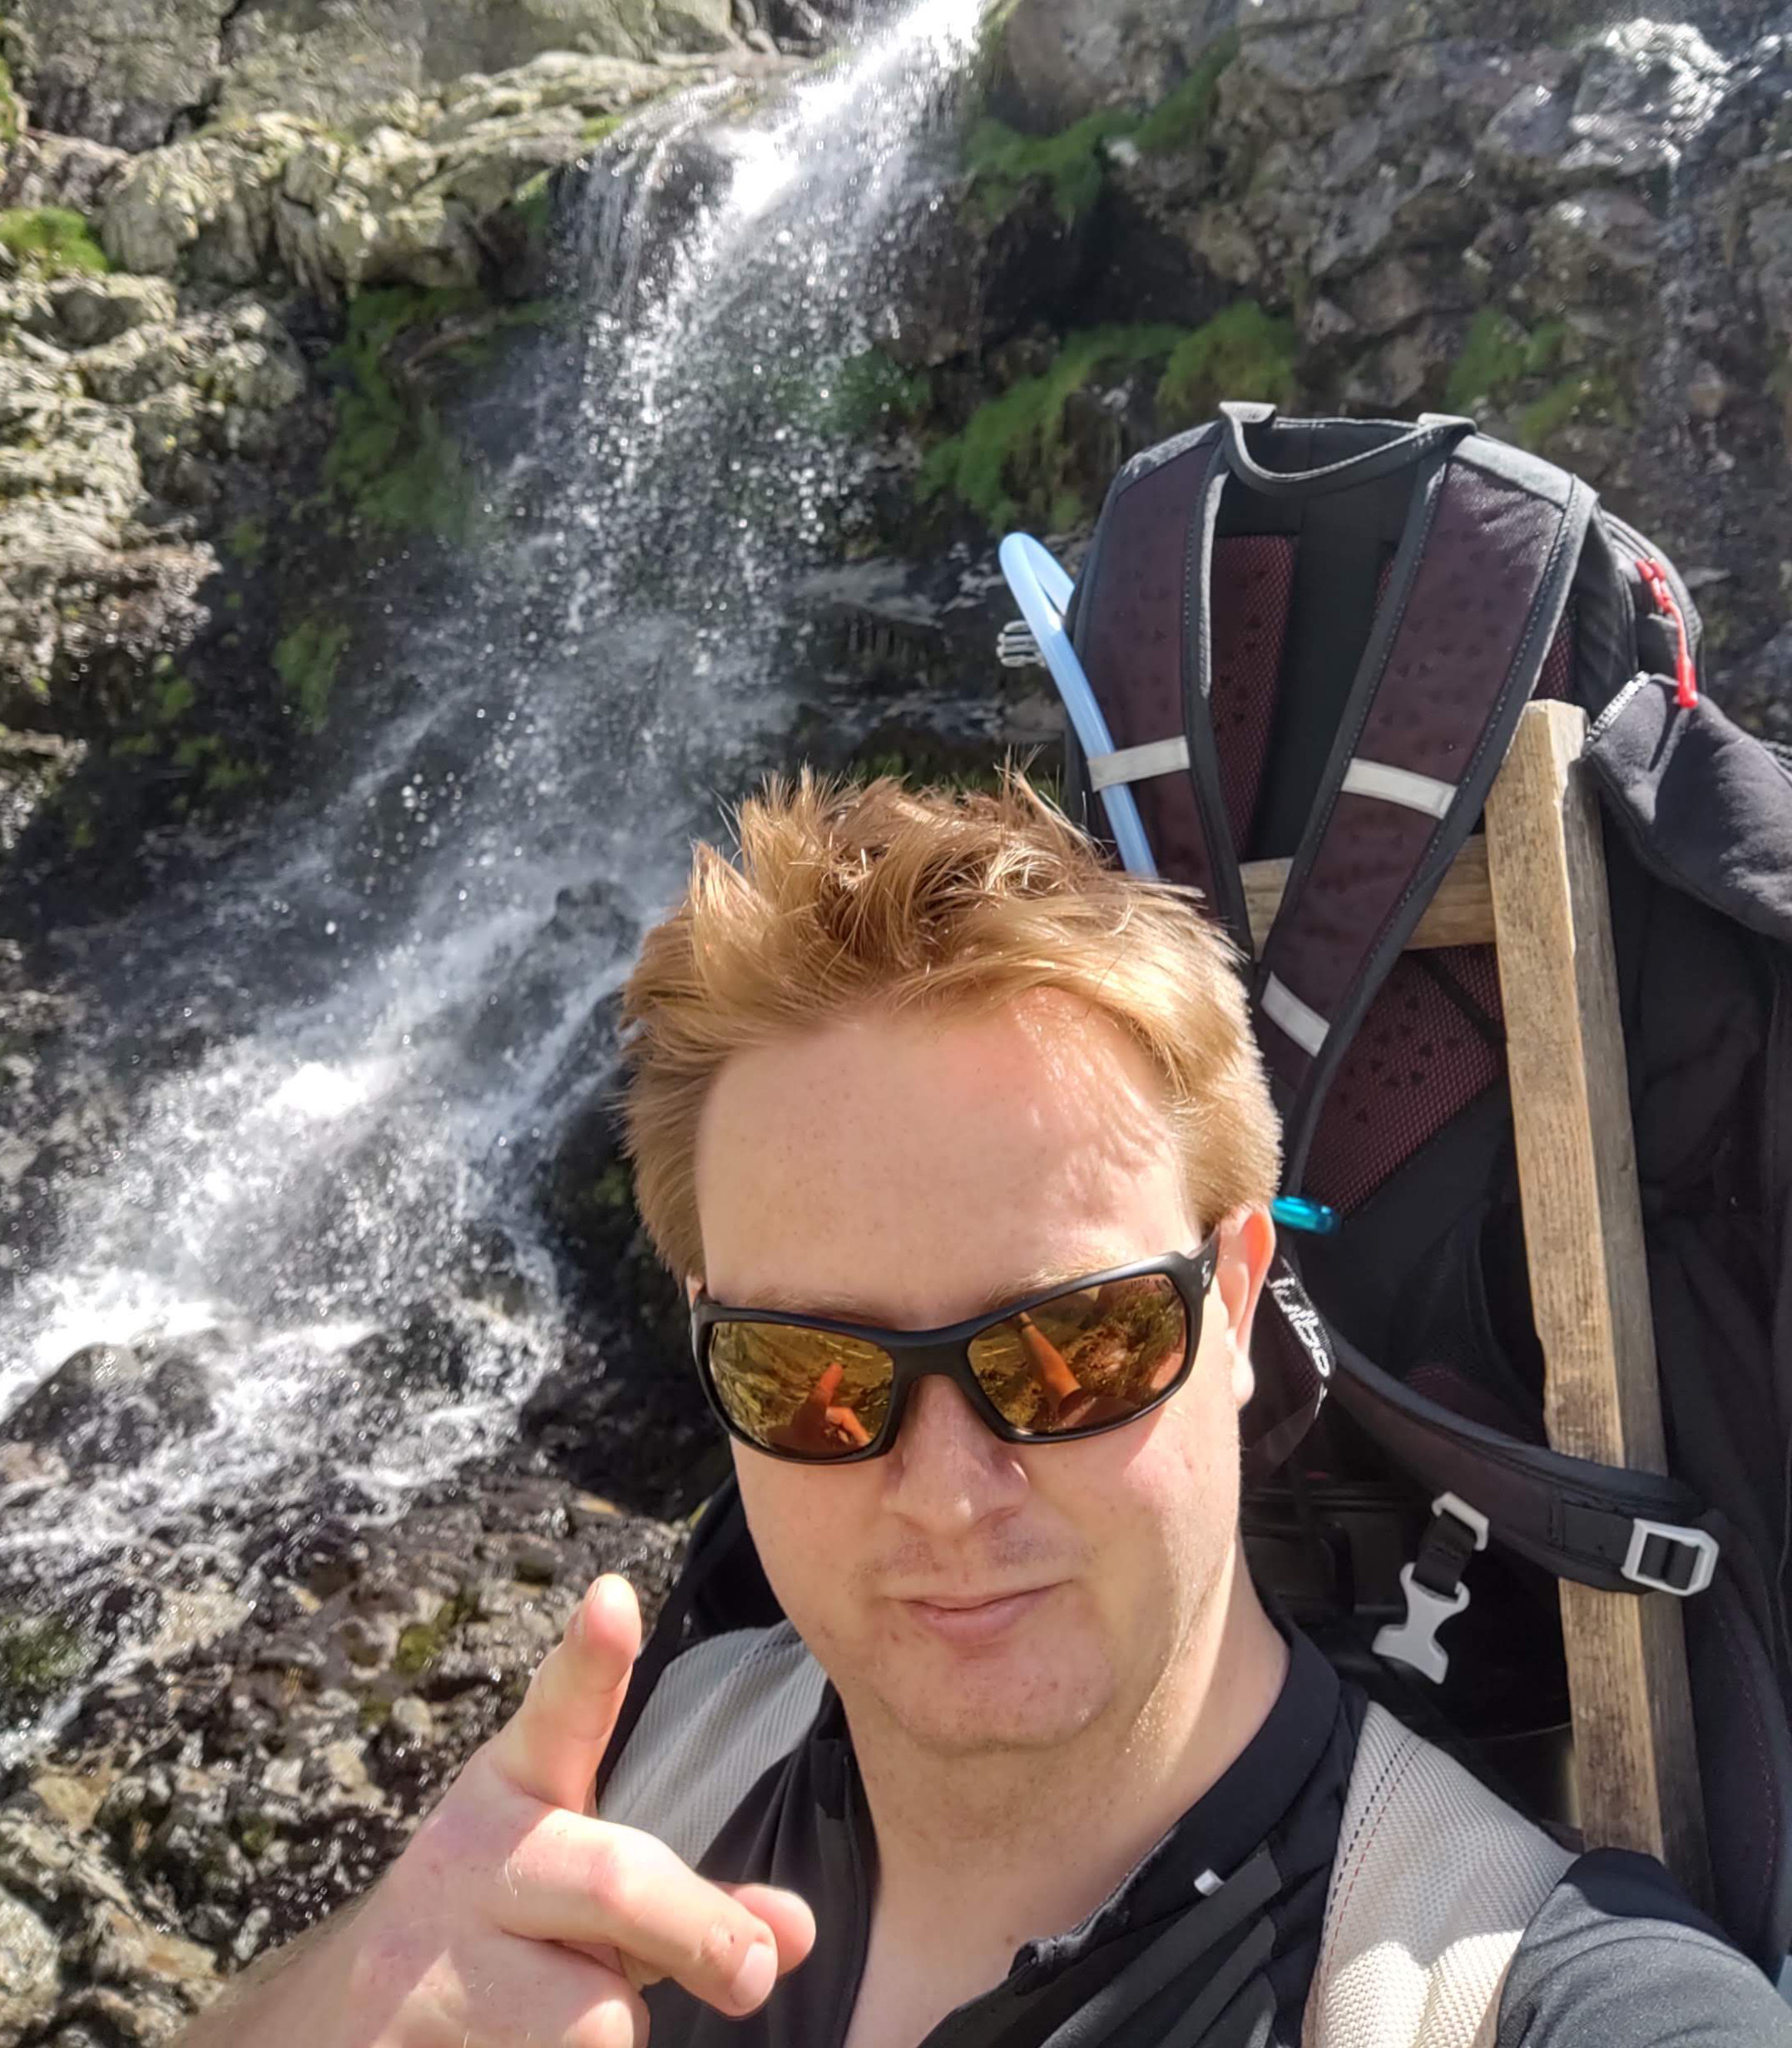
\includegraphics[scale=0.08]{../images/me.jpg}}
    \end{column}

    \begin{column}{0.5\textwidth}
      \begin{itemize}
        \item \url{https://github.com/michalnand/}
        \item \url{michal.nand@gmail.com}
      \end{itemize}
    \end{column}

  \end{columns}

    
\end{frame}

\end{document}